% !TEX TS-program = pdflatex
% !TEX encoding = UTF-8 Unicode

% This is a simple template for a LaTeX document using the "article" class.
% See "book", "report", "letter" for other types of document.

\documentclass[12pt]{scrreprt} % use larger type; default would be 10pt
\linespread {1,25}\selectfont %1.25 da er von Haus aus 1.2 ist und 1,25 * 1,2 = 1,5 isch
\usepackage[utf8]{inputenc} % set input encoding (not needed with XeLaTeX)
%
%\setkomafont{chapter}{\Large\linespread{ 1}\sffamily\bfseries}
%\setkomafont{section}{\Large\linespread{ 1}\sffamily\bfseries}
%%% Examples of Article customizations
% These packages are optional, depending whether you want the features they provide.
% See the LaTeX Companion or other references for full information.

%%% PAGE DIMENSIONS
\usepackage{geometry} % to change the page dimensions
\geometry{a4paper} % or letterpaper (US) or a5paper or....
% \geometry{margin=2in} % for example, change the margins to 2 inches all round
% \geometry{landscape} % set up the page for landscape
%   read geometry.pdf for detailed page layout information

\usepackage{graphicx} % support the \includegraphics command and options

% \usepackage[parfill]{parskip} % Activate to begin paragraphs with an empty line rather than an indent

%%% PACKAGES
\usepackage[german]{babel}
\usepackage{helvet}
\usepackage{amsmath}
\usepackage{hyperref}
\usepackage{amssymb}
\usepackage{gensymb}
\usepackage{picinpar}
\usepackage{float}
\usepackage{epsfig}
\usepackage{graphicx}
\usepackage[german]{varioref}
\usepackage{natbib}
%\usepackage{url}
\usepackage{breakurl}
\usepackage{calc}
\usepackage{color, listings}
\definecolor{brown}{cmyk}{0,0.81,1,0.60}
\definecolor{lightgray}{cmyk}{0.05,0.05,0.05,0.01}
%\usepackage{cite}
%\usepackage[round]{natbib}
%\bibliographystyle{alphadin}
%\usepackage[style=authoryear]{biblatex} %e
%\bibliographystyle{unsrt}
%\bibliography{literatur}
\usepackage{longtable} %for tables langer than a page
\usepackage{booktabs} % for much better looking tables
\usepackage{array} % for better arrays (eg matrices) in maths
\usepackage{paralist} % very flexible & customisable lists (eg. enumerate/itemize, etc.)
\usepackage{verbatim} % adds environment for commenting out blocks of text & for better verbatim
\usepackage{subfig} % make it possible to include more than one captioned figure/table in a single float
% These packages are all incorporated in the memoir class to one degree or another...

\renewcommand{\UrlBreaks}{\do\/\do\a\do\b\do\c\do\d\do\e\do\f\do\g\do\h\do\i\do\j\do\k\do\l\do\m\do\n\do\o\do\p\do\q\do\r\do\s\do\t\do\u\do\v\do\w\do\x\do\y\do\z\do\A\do\B\do\C\do\D\do\E\do\F\do\G\do\H\do\I\do\J\do\K\do\L\do\M\do\N\do\O\do\P\do\Q\do\R\do\S\do\T\do\U\do\V\do\W\do\X\do\Y\do\Z}


%%% HEADERS & FOOTERS
\usepackage{fancyhdr} % This should be set AFTER setting up the page geometry //fancyhdr
\pagestyle{fancy} % options: empty , plain , fancy
%\fancyhf{}
\renewcommand{\headrulewidth}{0.5pt} % customise the layout...
%\lhead{}\chead{}\rhead{}
%\lfoot{}\cfoot{\thepage}\rfoot{}
%\lohead{\headmark}


%%%% SECTION TITLE APPEARANCE
%\usepackage{sectsty}
%\allsectionsfont{\sffamily\mdseries\upshape} % (See the fntguide.pdf for font help)
% (This matches ConTeXt defaults)


\setkomafont{chapter}{\rm\bf \large} %Größe der Kapitelüberschriften
\setkomafont{section}{\rm\bf\large} %Größe der UNterkapitelüberschriften 
\setkomafont{subsection}{\rm\bf\large} %Größe der UNterkapitelüberschriften 

%%% ToC (table of contents) APPEARANCE
\usepackage[nottoc,notlof,notlot]{tocbibind} % Put the bibliography in the ToC
\usepackage[titles,subfigure]{tocloft} % Alter the style of the Table of Contents
\renewcommand{\cftsecfont}{\rmfamily\mdseries\upshape}
\renewcommand{\cftsecpagefont}{\rmfamily\mdseries\upshape} % No bold!


%\usepackage[automark]{scrpage2}
%\pagestyle{scrheadings}


%%% END Article customizations



%%% The "real" document content comes below...

\title{Entwicklung und Erprobung einer piezoresistiven Sensor-Schaltung mit drahtloser Energieversorgung im Projekt "MedLast"}
\author{Stephan Jobstmann}
\date{\today}
\pagenumbering{roman}

%\date{} % Activate to display a given date or no date (if empty),
         % otherwise the current date is printed 




\begin{document}
\maketitle
\setcounter {page}{1}
\def\chapterpagestyle{fancy}
\tableofcontents
\listoffigures
\lstlistoflistings
\listoftables
\lstset{language =C}
\lstset{basicstyle =\ttfamily \color{black}\small,
keywordstyle =\bfseries \color{blue},
commentstyle =\color{green},
numbers=left,
tabsize=4,
showspaces=false,           % Leerzeichen anzeigen ?
showtabs=false,             % Tabs anzeigen ?
extendedchars=true,         %
breaklines=true,            % Zeilen werden Umgebrochen
xleftmargin=27pt, %17pt
framexleftmargin=27pt, %17pt
framexrightmargin=5pt,
framexbottommargin=4pt,
backgroundcolor=\color{lightgray},
showstringspaces=false      % Leerzeichen in Strings anzeigen ? 
%numberstyle = \color{brown},
stringstyle =\itshape \color{red},
captionpos=b}
\chapter{Einleitung}
\pagenumbering{arabic}
Die moderne Schulmedizin ist mittlerweile an einem Punkt angelangt, an dem die biochemischen Prozesse innerhalb des Körpers als nahezu komplett erfasst gelten. Die Mechanismen der Informationsweitergabe über die Nervenbahnen, die Belastbarkeit der Anatomie oder die Zerlegungsprozesse des Stoffwechsels sind als solche weitestgehend erforscht. Wie jedoch in jedem Forschungsbereich bedeutet dies auch, dass die Lernkurve beziehungsweise die Anzahl der Ergebnisse an innovativen Erkenntnissen drastisch über die letzten Jahrzehnte abnehmen. Weiter lässt sich feststellen, dass die Fortschritte der modernen Medizin sich hauptsächlich auf die Innovationen aus den Bereichen der Pharmazie und der Medizintechnik berufen. So ermöglichen intelligente Kamerasysteme eine bessere Überwachung von Operationen am schlagenden Herzen\footnote{Motion Compensation in Minimally Invasive Heart Surgery \citep{DLR}} oder die Abnahme von elektrischen Nervensignalen eine Steuerung von kybernetischen Prothesen\footnote{Paralyzed individuals control robotic arms to reach and grasp using brain computer interface \citep{DLR2}}.\\
Die fortschreitende Entwicklung in der Medizintechnik bietet auch Hilfestellung im Genesungsprozess im Fachbereich der Orthopädie. So wird im Projekt "`MedLast"' sowohl eine Unterstützung für den Patienten als auch eine Kontrollmöglichkeit während der Heilung einer Beinfraktur erstrebt. Dabei wird das Gewicht auf dem geschienten Fuß und die Häufigkeit der Auftritte aufgezeichnet. Gleichzeitig sollen diese Daten zur zeitnahen Kontrolle an eine visuelle Ausgabeeinheit, ähnlich einer Armbanduhr, weitergegeben werden. Für die Konstruktion der Elektronik, welche die Werte für Belastung und Schrittzahl aufnimmt, werden die Gebiete Energieversorgung und Sensorik zusammengefasst. Hierbei kann nur sehr schlecht auf proprietäre Komplettlösungen zurückgegriffen werden. Darum sollen in dieser Arbeit die nötigen Schritte unternommen werden, um ein solches System zu erstellen und in Betrieb zu nehmen.
\chapter{Anforderungen}
Als wesentliche Bestandteile der Aufgabenstellung sind zuerst die zu bearbeitenden Teilgebiete zu nennen. Hierzu gehören:
\begin{itemize}
\item
Energiezuführung
\item
Energiebereitstellung
\item
Sensorik-Auswertung
\end{itemize}
Bei der Energiezuführung sollen dahingehend Überlegungen angestrebt werden, auf welche Art und Weise das komplette Modul mit Spannung versorgt werden kann. Dabei sollen autarke wie auch fremd-gespeiste Quellen betrachtet werden. Die Energiebereitstellung bezieht sich auf die Speicherung im oder am Modul selbst. Hierbei ist die Abstimmung zwischen Bedarf und Bereitstellung ausschlaggebend für die Wahl der zu verwendenden Technologie. In der Sensorik-Auswertung ist natürlich in erster Linie der zu verwendende Sensor bestimmend. Da dieser sich durch den steten Optimierungsverlauf auch im Verhalten sowie in den zu erwartenden Messgrößen ändern kann, sollte diesbezüglich ein Freiheitsgrad in der Implementierung vorhanden sein. Weiter soll im zentralen Mikrocontroller des Moduls eine passende Auslesesoftware erstellt werden. Diese muss die gemessenen Daten aufbereiten und in eine passende SI-Einheit wie Newton [N] oder Kilogramm [kg] zurück rechnen. Als kleinere Additive sind folgende elektronische Komponenten noch vorgesehen: 
\begin{itemize}
\item
Piezo-Summer samt Treiberschaltung
\item
Schutzbeschaltung
\item
Temperaturaufnehmer
\end{itemize}
\chapter{Grundlagen}
\section{Energy-Harvesting}
\subsection{Piezoelektrisch}

Eines der größten abgedeckten Felder im Energy-Harvesting Bereich ist die Gewinnung von nutzbarer elektrischer Energie aus vorhandener mechanischer Energie. Hierbei werden die piezoelektrischen Effekte genutzt, welche bei Druck oder Schwingungsbelastungen auf einem Piezokristall entstehen \citep[vgl. S.36 ff]{Dembowski2011}. Dabei entsteht bei bestimmten nichtleitenden Keramiken aufgrund von mechanischem Druck elektrische Ladung an den Oberflächen. Die inneren Ladungskerne driften dabei auseinander, es bildet sich ein Dipol aus. Es werden die grundlegenden Gleichungen des Piezo-Effekts wie folgt beschrieben:
\begin{align}
D & =  \textrm{d} \cdot T + \varepsilon^{\textrm{T}} \cdot E\\
S & =  s^{\textrm{E}} \cdot T + \textrm{d} \cdot E
\end{align}
Mit den Parametern:
\begin{array}[t] {r c l}
D & : & \textrm{Dielektrische Verschiebung (statt Polarisation)}\\
S & : & \textrm{Relative mechanische Dehnung} \\
T & : &\textrm{Mechanische Spannung} \\
E & : & \textrm{Elektrische Feldstärke} \\
  $d$  & : & \textrm{piezoelektrische Ladungskonstante} \\
 s^{\textrm{E}}  & : & \textrm{Elastizitätskonstante, E = konstant} \\
 \varepsilon^{\textrm{T}}  & : & \textrm{Permittivität, T = konstant}\\
\end{array}\\ \newline
Zum Energy-Harvesting werden bevorzugt Biegebalken\footnote{im Englischen auch bekannt als Cantilever} verwendet. Diese können technologisch an die angeforderte Kraftaufnahme, die Schwingungsfrequenz und die Amplitude der resultierenden Spannung angepasst werden. Der Aufbau als Biegebalken liefert sein Optimum der Energieumwandlung bei seiner Resonanzfrequenz. Dabei wird weiter zwischen Transversalschwingern\footnote{31-Schwingungsmodus} (Formel \ref{formel:3.3} und \ref{formel:3.4}) und Longitudinalschwingern\footnote{33-Schwingungsmodus}  (Formel \ref{formel:3.5} und \ref{formel:3.6}) unterschieden. 
\begin{align}
D_3 & =  \textrm{d}_{31} \cdot T_1 + \varepsilon_{33}^{\textrm{T}} \cdot E_3 \label{formel:3.3} \\
S_1 & =  s_{11}^{\textrm{E}} \cdot T_3 + \textrm{d}_{31} \cdot E_3 \label{formel:3.4}
\end{align}
Bei den Transversalschwingern wird quer zur mechanischen Auslenkung eine elektrische Spannung erzeugt. Wenn mechanische Schwingung bzw. Druckbelastung mit dem elektrischen Feld bzw. der dielektrischen Verschiebung gleichgerichtet ist, wird von Longitudinalschwingern gesprochen. Transversalschwinger erzeugen eine rund zehnmal höhere Spannung als Longitudinalschwinger \citep[S.39]{Dembowski2011}. Ein Beispiel für die Wirkungsweise im kristallinen Aufbau eines longitudinal aktiven Piezoelements ist in Abbildung \vref{piezo} zu sehen. Dabei ist recht deutlich die Ladungsverschiebung aufgrund der Verzerrung der Kristallstruktur zu erkennen. 
\begin{align}
D_3 & =  \textrm{d}_{33} \cdot T_3 + \varepsilon_{33}^{\textrm{T}} \cdot E_3 \label{formel:3.5} \\
S_3 & =  s_{33}^{\textrm{E}} \cdot T_3 + \textrm{d}_{33} \cdot E_3 \label{formel:3.6}
\end{align}
\begin {figure}[htbp]
\caption[Longitudinaler Piezoeffekt; Kristallstruktur und Ladungsverschiebung]{Longitudinaler Piezoeffekt; Aufbau der Kristallstruktur und Ladungsverschiebung}
      \begin{center}
       \fbox{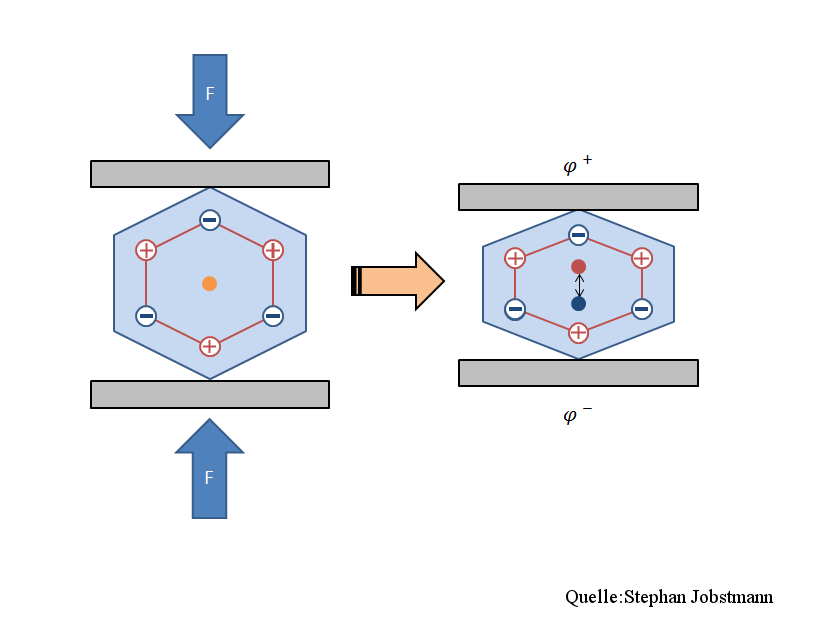
\includegraphics[width=1\textwidth-2\fboxsep-2\fboxrule]{Bilder/Piezo.png}}
      \end{center}
Quelle: Universität Bayreuth Didaktik der Chemie \citep{BAY}
\label{piezo}
\end{figure}
\subsection{Thermoelektrisch}
Eine im Vergleich zu piezoelektrischem Energy-Harvesting hohe Energieumwandlung wird mit der thermoelektrischen Transformation erzielt. Dabei wird als physikalische Grundlage der Seebeck-Effekt benutzt. Dieser beschreibt, dass bei zwei unterschiedlichen Metalllegierungen bei vorliegender Differenz der Temperaturen am Übergang der Elemente eine Spannung entsteht. Die entstandene Potentialdifferenz wird auch Thermospannung \citep[vgl. S.158]{Schruefer2012} genannt. Die Inverse dieses Vorgangs wird mit dem Peltier-Effekt beschrieben. Da das Verhalten der spezifischen Elemente reziprok ist, können Peltierelemente auch zur Gewinnung von elektrischer Energie genutzt werden. \newline
Der Seebeck-Effekt beruht auf den folgenden molekularen Gegebenheiten: Naturgemäß wandern bei einem Metall, welches einem Temperaturunterschied ausgesetzt ist, die Elektronen von der heißen zur kalten Seite. Dies geschieht aufgrund der natürlichen Diffusionsbewegung innerhalb des Metalls. Bei zwei aneinanderliegenden, verlöteten oder verschweißten Legierungen gibt das Metall mit der niedrigeren Austrittsarbeit Elektronen an das andere Metall ab und wird dadurch positiv geladen. Dadurch bildet sich an der Kontaktfläche ein elektrisches Feld. Dieses kann resultierend als direkte Proportionale zur anliegenden Temperaturdifferenz der zwei Kontaktstellen mit einem Voltmeter gemessen werden. Übliche Werte hierfür sind ca. $10  \frac{\textrm{mV}}{100 \degree \textrm{K}}$. Durch intelligente Beschaltung, zum Beispiel mehrere Elemente in Reihe, lässt sich eine höhere Empfindlichkeit erzielen. Mit dem in Kapitel \vref{energy} vorgestellten LTC3108 Baustein lässt sich ab einer Ausgangsspannung von 20mV eine stabile Energieumwandlung in Gang bringen. \newline \newline
Wird der technischen Aufbau nun so gestaltet, dass er zur Energieumwandlung und nicht zur Temperaturmessung verwendet werden soll, erweist es sich als nützlich ein oder mehrere Peltierelemente im umgekehrten Betrieb zu verwenden. \citep[vgl. S.30]{Dembowski2011}
\section{Drahtlose Energieübertragung}
Das hier vorgestellte Konzept bezieht sich auf Technologie, die mit dem WPC\footnote{Wireless Power Consortium}-Standard konform ist. Es gibt auch andere Konzepte, die sich mit drahtloser Energieübertragung beschäftigen. Das ist auch nachvollziehbar wenn man bedenkt, dass die ersten drahtlosen Anlagen von Nikola Tesla bereits 1895 in Betrieb genommen wurden\citep{TESLA}. Allerdings weisen die meisten einfacheren Aufbauten einen entscheidenden Nachteil auf: Sie sind nicht geregelt. Der WPC-Standard hat aber nicht nur das Regelungssystem als Vorteil gegenüber anderen Konzepten vorzuweisen. In den nachfolgenden Unterkapiteln werden die einzelnen Punkte der Spezifikation aufgeführt und erklärt. Dabei ist der Inhalt sinngemäß aus Quelle \citep{WPC} genommen.
\subsection{Prinzip}
Das zugrundeliegende Prinzip



\section{Lithium-Ionen Akkumulator}
Der LiIon-Akku\footnote{Lithium-Ionen Akkumulator} stellt den aktuellen Stand der Technik in der elektrischen Speichertechnologie dar. Da dieser auch in dieser Arbeit zum Einsatz kommt, sollen im Folgenden die wichtigsten Eckdaten und Informationen bezüglich dessen Verwendung näher erläutert werden. Der Inhalt wurde sinngemäß aus der Webseite Battery University \citep{BAT} übernommen.
\subsection{Aufladen}
Der Ladeprozess ähnelt dem von Blei-Akkumulatoren. Im Gegensatz zu Diesen ist allerdings auf die Speisespannung genauestens zu achten. Einzelne Zellen werden mit einer Spannung von 4,20V geladen. Dabei darf die anliegende Spannung höchstens $\pm$50mV vom Normalwert abweichen. Andernfalls ist mit einer Verkürzung der Lebensdauer der Akku-Zelle zu rechnen. Anders als bei anderen Akkumulatoren wie dem NiMH\footnote{Nickel-Metallhydrid}-Akku ist auch keine sogenannte Erhaltungsladung\footnote{besser bekannt unter dem englischen Begriff: trickle charging} zulässig. In Abbildung \vref{fig:bat} sind die einzelnen Schritte des Ladevorgangs zu sehen. Diese werden im Folgenden näher erklärt.
\begin {figure}[htbp]
\caption{Ladungskurve eines typischen Lithium-Ionen-Akkumulators}
      \begin{center}
       \fbox{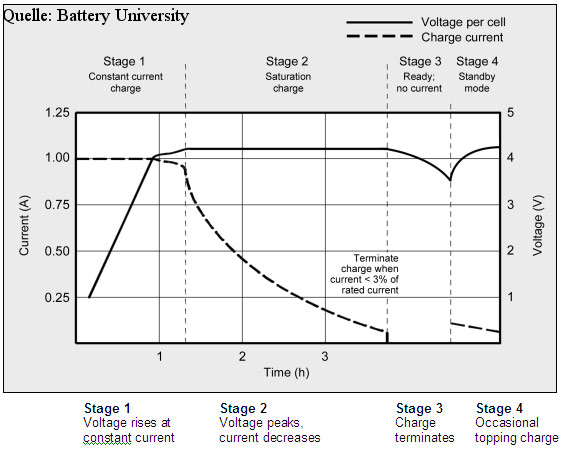
\includegraphics[width=1\textwidth-2\fboxsep-2\fboxrule]{Bilder/ion1.jpg}}
      \end{center}
Quelle: Cadex Electronics Incorporated \citep{BAT}
\label{fig:bat}
\end{figure}
\subsubsection{Phase 1}
In der ersten Phase des Ladevorgangs wird der Akku mit einem konstanten Ladestrom gespeist. Dabei wird die Höhe in der Einheit $C$ festgelegt. Diese ist nicht zu verwechseln mit der Bezeichnung der Ladung, $Coulomb$. Stattdessen handelt es sich um einen Umrechnungsfaktor, ausgehend vom Quotienten $\frac{Ladestrom}{Kapazit"at}$ beziehungsweise $1\frac{A}{Ah}$. Dabei wird das resultierende $\frac{1}{h}$ in der Literatur ignoriert und man spricht generell von $C$. Übliche Werte hierfür bewegen sich zwischen 0,5 und 1$C$. Ein Ladestrom von 0,7$C$ hat als resultierenden Strom 1,4A bei einer 2Ah Zelle. Allerdings ist es für die Zelle auch nicht schädlich, wenn sie weit unter diesen Werten bestromt wird. So können LiIon-Zellen beispielsweise auch mit Solarzellen oder anderen Niederstrom-erzeugenden Quellen gespeist werden.
\subsubsection{Phase 2}
Wenn beim Laden mit konstanten Strom der Spannungswert von 4,05V erreicht wird, ändert sich die Ladestrategie. Nun wird eine konstante Spannung von 4,2V an die Zelle angelegt. Dabei wird der Ladestrom weiter gemessen, denn an ihm wird das Abbruchkriterium festgelegt. Erreicht der Strom 3\% des in der ersten Phase festgelegten Werts, so ist der Akku fertig geladen und die Zelle gesättigt. Auch hier sei angemerkt, dass die maximale Spannung von 4,2V nicht zwingend erreicht werden muss. Wird die Zelle bei einer Spannung von 4,1V geladen, erreicht sie nicht die maximale Kapazität. Dafür kann Sie öfter geladen werden, die Ladezyklenzahl erhöht sich.
\subsubsection{Phase 3}
Diese Phase beschreibt lediglich den Arbeitszustand des Akkus. Dabei sinkt vorerst die Spannung der Zelle rapide von dem zuvor angelegten Ladungshöchstwert von 4,2V auf eine Nennspannung von 3,6 bis 3,7V.  Auf diesem Wert hält sich die Spannung relativ lange, bis dieser kurz vor der vollständigen Entladung steht. Erst dann beginnt die Spannung wieder weiter zu sinken. Je nach Herstellerempfehlung befindet sich die Entladeschlussspannung zwischen 2,5 und 3V. Wird der Akku dennoch weiter entladen, können entweder Schäden auftreten oder er muss mit einem anderen Ladeprofil wieder regeneriert und vorgeladen werden.
\subsubsection{Phase 4}
Soll der Akku auf Bereitschaft geladen werden, so darf dieser nicht mit einer Erhaltungsladung bestromt werden. Stattdessen wird die Spannung der Zelle gemessen und bewertet. Fällt diese unter einen Schwellwert von meistens 4,05V wird mit Phase zwei wieder nachgeladen, bis das Abbruchkriterium des Ladestroms erreicht worden ist.
\subsection{Allgemeine Hinweise}
\begin{itemize}
\item
LiIon Akkus sollten nie unter 2,7V per Zelle entladen werden. Daher sollte bei der Einlagerung darauf geachtet werden, dass eine Mindestladung von 40\% der Maximalkapazität vorhanden ist.
\item
Bei einem gewöhnlichen Ladevorgang ist eine Temperaturerhöhung der Zelle von 5-10$\celsius$ üblich. Höhere Temperatursprünge sind ein Zeichen für eine vorangegangene, unsachgemäße Handhabung oder Schäden am Akku. 
\item
LiIonen Akkus sollten generell bei moderaten Temperaturen betrieben werden. Insbesondere beim Laden sollte darauf geachtet werden, dass die Temperatur 0$\celsius$ nicht unterschritten wird.
\item
Tiefentladene Akkus können mit einem speziellen Ladeprofil eventuell wieder aktiviert werden.
\item
Eine vollständige Ladung beziehungsweise Entladung wie bei NiMH-Akkus ist nicht förderlich für dessen Lebensdauer. Teilaufladungen sind bei diesem Akkutyp besser.
\end{itemize}
%%%%%%%%%%%%%%%%%%%%%%%%%%%%%%%%%%%%%%%%%%%%%%%%%%%%
\chapter{Voruntersuchung}

\section{Motivation}
Ausschlaggebend für diese Messungen ist die Bestimmung von mechanischen Lastwechseln im niederfrequenten Bereich unter 4Hz. Genauer handelt es sich dabei um die Erfassung der Druckbelastung einer medizinischen Schienung eines verletzten Beines, mithilfe von piezoeletrischen Elementen. Diese Messung sollte bereits im Vorfeld der Arbeit eine Aussage zulassen, welche Methode, piezokapazitiv oder piezoresistiv, zur Bestimmung der anliegenden mechanischen Last den größeren Vorteil bietet. Bei diesen Bauelementen können anhand von drei Parametern Rückschlüsse auf die mechanische Belastung gezogen werden:
\begin{itemize}
\item Spannung,
\item Ladung,
\item Kapazität.
\end{itemize}
Dieses Kapitel bezieht sich auf die Untersuchung von Abhängigkeiten zwischen mechanischer Druckbelastung und elektrischer Kapazitätsänderung am Piezoelement. Weiter ist es zu großen Zügen dem Vorbericht \citep{Jobstmann2012} wörtlich entnommen.
\section{Versuchsaufbau}

Ziel dieser Versuchsreihe ist die Bestimmung der Kapazitätsänderung von piezoelektrischen Elementen bei mechanischer Druckbelastung. Dabei wird das Piezoelement elektrisch isoliert in einem Schraubstock belastet. Über Zuleitungen wird mit einem sogenannten LCR-Meter eine Vierdraht-Impedanz-Messung durchgeführt, die einzelnen Parameter hierfür werden bei den Versuchsreihen angegeben. Mithilfe einer Kraftmessdose, welche eine Vollmessbrücke mit Dehnmessstreifen beinhaltet, wird der angelegte mechanische Druck am Piezoelement abgeleitet. Da zu Messbeginn nur geringe Zusatzinformationen zu diesem Hilfsmittel vorhanden waren, geschahen alle Auswertungen in einem geringen Bereich unterhalb der Maximalbelastbarkeit von 250N. Weiter ist die angelegte Versorgungsspannung an der Messdose stets 10V DC. bei allen Messungen wurde ein LCR-Meter ISO-TECH LCR-821 zur Impedanzmessung und ein Fluke-Hand-Multimeter 179 zur Spannungsmessung verwendet. Als Spannungsquelle stand ein Hameg HM8142 bereit.

\section{Ergebnis}

Im Allgemeinen lassen sich aufgrund der getätigten Messungen folgende Aussagen treffen:
\begin{itemize}
\item
Die Kapazitätsänderung der Piezoelemente unter Last stellt für kleine wirkende Kräfte keine hinreichend reproduzierbare Methode zur Messung von mechanischer Druckbelastung dar. Aufgrund der massiv einwirkenden parasitären Effekte, seien es Veränderungen der Luftfeuchte, Temperaturschwankungen oder pyroelektrische Einflüsse, konnten keine eindeutig wiederholbaren Werte erzielt werden.
\item
Die Werkstoffstabilität ist auch in Frage zu stellen. Während der Messung ist ein Element unter Belastung zu Bruch gegangen.
\item
Weiter lassen sich die Ergebnisse der einzelnen Prüflinge unterscheiden:
\begin{itemize}
\item
CeramTec, P502, einschichtiger Piezo: Bei steigender Belastung verläuft die dazu korrespondierende Kapazitätskurve wie eine Exponentialfunktion mit negativem Exponenten. Weiter ist dieser während der Messung bei einer nicht mehr nachvollziehbaren Belastung zerbrochen. Die Reproduzierbarkeit einzelner Messergebnisse ist nahezu ausgeschlossen.
\item
CeramTec, P505, Mehrschichtiger Piezo: Auch bei diesem Piezoelement verläuft unter steigender Belastung die dazugehörige Kapazitätskurve monoton fallend. Weiter wurde auch hier eine hohe Abhängigkeit von äußeren Einflüssen festgestellt.
\item
Elliptec, Mehrschichtiger Piezo: Bei diesem Stack ergab sich eine mit dem Druck steigende Kapazitätskurve. Allerdings erschwerten auch hier parasitäre Effekte eine eventuelle Reproduzierbarkeit.
\end{itemize}
\end{itemize}


\section{Messungen}

\subsection{Sonox P502} 
Bei diesem Piezobaustein handelt es sich um ein einfaches, nicht mehrschichtiges Element. Die nachfolgenden Messungen untersuchten das Verhalten der Kapazität unter mechanischer Druckbelastung entlang der elektrischen Feldorientierung. Entgegen der Erwartung, dass die Kapazität mit steigender Druckbelastung ebenfalls steigt, verhält sich diese mehr wie eine Exponentialfunktion mit negativen Exponenten. Dies ist in nahezu allen folgenden Graphen der kommenden Unterkapitel nachzuvollziehen.
%%%%%%%%%%%%%Kapazität über steigender Druckbelastung%%%%%%%%%%%%%%%
\subsubsection{Kapazität über steigender Druckbelastung}
Diese Messung zeigt das kapazitive Verhalten des Piezoelements Sonox P502. Bei den Messwerten wird die Kapazität über die angelegte Kraft, bzw. die Spannung an der Kraftmessdose, aufgetragen, wie in Tabelle \vref{tab:2.1} und Abbildung \vref{fig:2.1} nachzuvollziehen ist. Speisefrequenz der Impedanzmessung war 500Hz bei 1V Amplitude.
\setlongtables
\begin{longtable}{| l | l | l |}
\caption[Messung 1; Sonox 502 Kapazitives Verhalten]{Messung 1; Sonox 502 Kapazitives Verhalten über steigende mechanische Belastung}\\
\hline
$U_{diff}$ in mV&$C_{diff}$ in nF&$C_{Piezo}$ in nF\\
\hline
\endfirsthead
\hline
$U_{diff}$ in mV&$C_{diff}$ in $nF$&$C_{Piezo}$ in nF\\
\hline
\endhead
\hline
\multicolumn{3}{|c|}{Fortsetzung auf der nächsten Seite}\\
\hline
\endfoot
\hline \hline
\endlastfoot
\hline
\label{tab:2.1}%
0.02&-0.01795&\\
0.50&-0.0235&\\
0.94&-0.02212&\\
1.48&-0.0235&0.9766\\
1.93&-0.0244&0.9754\\
2.49&-0.02529&0.9748\\
3.00&-0.02801&0.9716\\
3.60&-0.0294&0.9705\\
4.10&-0.02995&0.96981\\
4.56&-0.03057&0.96935\\
5.00&-0.03137&0.96858\\
5.51&-0.03184&0.96811\\
6.11&-0.03231&0.96766\\
\end{longtable}
\begin {figure}[htbp]
	\caption[Messung 1; Sonox 502 Kapazitives Verhalten]{Messung 1; Sonox 502 Kapazitives Verhalten über steigende mechanische Belastung}
      \begin{center}
\fbox{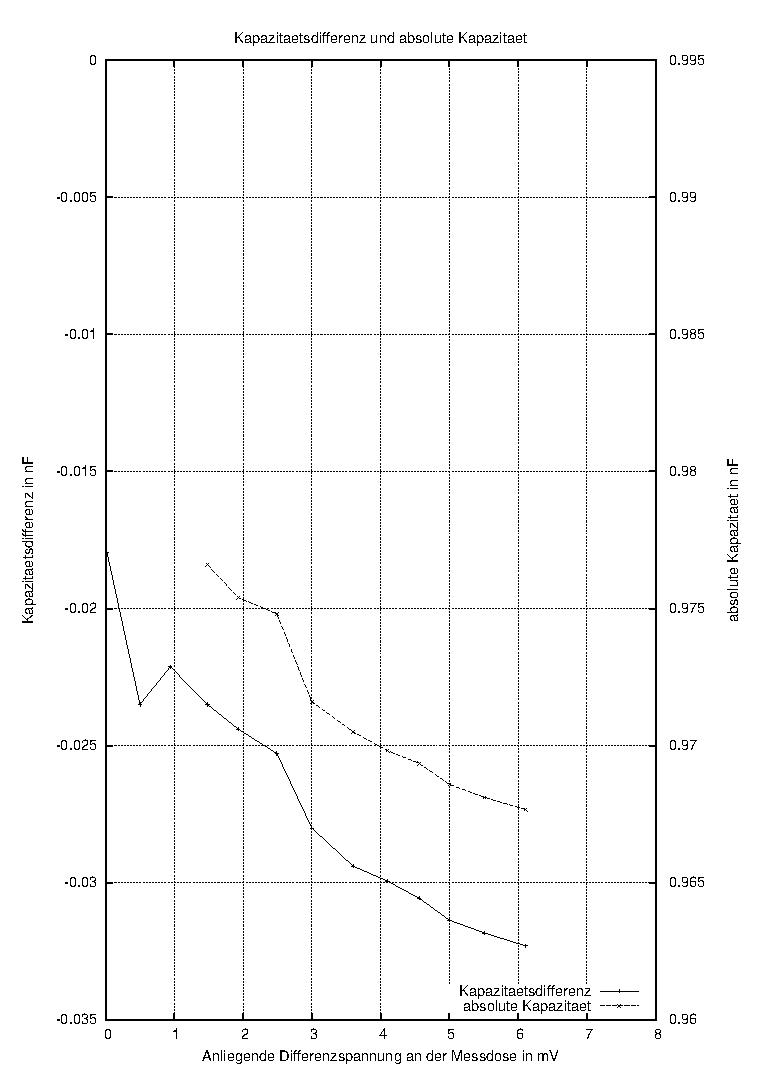
\includegraphics[width=0.8\textwidth-2\fboxsep-2\fboxrule]{tabelle2_1_1}}
      \end{center}
Quelle: Stephan Jobstmann
\label{fig:2.1}
\end{figure}

%%%%%%%%%%%Kapazität über statischer Druckbelastung%%%%%%%%%%%%%%%
\subsubsection{Kapazität über statischer Druckbelastung}
Durch die bei der ersten Messung stets ändernden Kapazitäten während einer Druckvorgabe wird dieser Versuch zur Untersuchung bei statischer Belastung angesetzt. Durch die Beobachtung der sinkenden Spannungsdifferenz (der Kraftmessdose) über die Zeit lässt sich die auftretende Kapazitätsänderung (des Piezoelements) auf die elastischen Kunststoffbacken des Schraubstocks zurückführen. Die Werte bzw. die grafische Auswertung ist hierbei aus der Tabelle \vref{tab:2.2} und dem Graphen aus Abbildung \vref{fig:2.2} zu entnehmen. \\
Aufgrund eines Gegenvergleichs lässt sich an dieser Stelle bereits sagen, dass die sich verringernden Werte auf die fortwährende Entspannung der Kunststoffbacken des Schraubstocks zurückführen lässt.

\setlongtables
\begin{longtable}{| l | l | l |}
\caption[Messung 2; Sonox 502 Statisches Verhalten]{Messung 2; Sonox 502 Statisches Verhalten über steigende mechanische Belastung}\\
\hline
Uhrzeit&$U_{diff}$ in mV&$C_{Piezo}$ in nF\\
\hline
\endfirsthead
\hline
Uhrzeit&$U_{diff}$ in mV&$C_{Piezo}$ in nF\\
\hline
\endhead
\hline
\multicolumn{3}{|c|}{Fortsetzung auf der nächsten Seite}\\
\hline
\endfoot
\hline \hline
\endlastfoot
\hline
\label{tab:2.2}%
09:50:00&10.12&0.9734\\
10:20:00&9.59&0.9662\\
11:40:00&9.37&0.96311\\
\end{longtable}

\begin {figure}[htbp]
\caption[Messung 2; Sonox 502 Statisches Verhalten]{Messung 2; Sonox 502 Statisches Verhalten über steigende mechanische Belastung}
      \begin{center}
\fbox{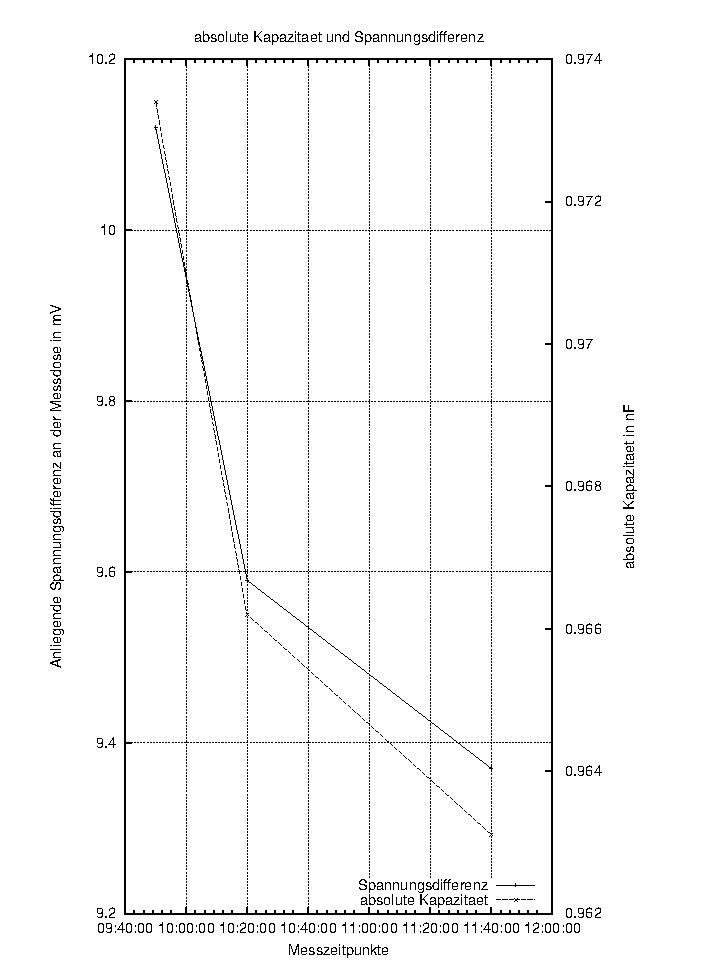
\includegraphics[width=0.8\textwidth-2\fboxsep-2\fboxrule]{tabelle2_1_2}}
      \end{center}
Quelle: Stephan Jobstmann
\label{fig:2.2}
\end{figure}
\newpage
%%%%%%%%%%%%%%Weitere Messung mithilfe des Maschinenschraubstocks%%%%%%%%%%%%%
\subsubsection{Weitere Messung mithilfe des Maschinenschraubstocks}
Bei vorhergehenden Messungen ergab sich der Verdacht, dass die Werte aufgrund der nicht konstanten Druckbelastung durch die Spannvorrichtung verfälscht worden sind. Darum ist diese Messreihe mit einem schweren Maschinenschraubstock mit Stahlbacken erstellt worden. Hierbei wurde zusätzlich noch der Einfluss eines Parallelwiderstands untersucht. Allerdings wurden die Messungen jeweils nach einer Abschätzung der auftretenden Messwertdifferenz abgebrochen, da dies nicht als zielführend erschien. Zum Sicherstellen dieser Annahme wurde jeweils noch ein Messwert bei einer Druckbelastung von einer äquivalenten Spannung von 10mV aufgenommen. Diese ergaben keine feststellbaren Unterschiede zu den letzten dokumentierten Werten. Bei den Messungen wurde jeweils eine Entspannungsphase der Belastungsvorrichtung von 2 Minuten bei jedem Messschritt eingehalten. Die erzielten Messergebnisse sind in den Tabellen \vref{tab:2.3} und \vref{tab:2.4} ersichtlich. Anhand der Abbildung \vref{fig:2.3} lässt sich die unveränderte Charakteristik des Verhaltens unter Last nachvollziehen. Die Skalierung wurde hier zur Veranschaulichung angepasst. 

\setlongtables
\begin{longtable}{| l | l |}
\caption{Messung 3; mit 100k$\Omega$ Parallelwiderstand}\\
\hline
$U_{diff}$ in mV&$C_{Piezo}$ in nF\\
\hline
\endfirsthead
\hline
$U_{diff}$ in mV&$C_{Piezo}$ in nF\\
\hline
\endhead
\hline
\multicolumn{2}{|c|}{Fortsetzung auf der nächsten Seite}\\
\hline
\endfoot
\hline \hline
\endlastfoot
\hline
\label{tab:2.3}%
0.44&0.9719\\
0.97&0.9685\\
1.75&0.9675\\
2.36&0.9665\\
3.00&0.9654\\
3.53&0.9645\\
4.03&0.9643\\
4.53&0.963\\
5.05&0.9625\\
5.78&0.9626\\
6.38&0.9625\\
\end{longtable}

\setlongtables
\begin{longtable}{| l | l |}
\caption{Messung 4; ohne Parallelwiderstand}\\
\hline
$U_{diff}$ in mV&$C_{Piezo}$ in nF\\
\hline
\endfirsthead
\hline
$U_{diff}$ in mV&$C_{Piezo}$ in nF\\
\hline
\endhead
\hline
\multicolumn{2}{|c|}{Fortsetzung auf der nächsten Seite}\\
\hline
\endfoot
\hline \hline
\endlastfoot
\hline
\label{tab:2.4}%
0.64&0.9683\\
1.26&0.9640\\
1.75&0.9620\\
2.40&0.9603\\
2.87&0.9587\\
3.88&0.9570\\
4.38&0.9540\\
5.22&0.9538\\
\end{longtable}

\begin {figure}[htbp]
\caption[Messung 3 und 4; Sonox 502 unter Einsatz besserer Spannvorrichtung]{Messung 3 und 4; Sonox 502 Kapazitives Verhalten über steigende mechanische Belastung unter Einsatz besserer Spannvorrichtung}
      \begin{center}
  \fbox{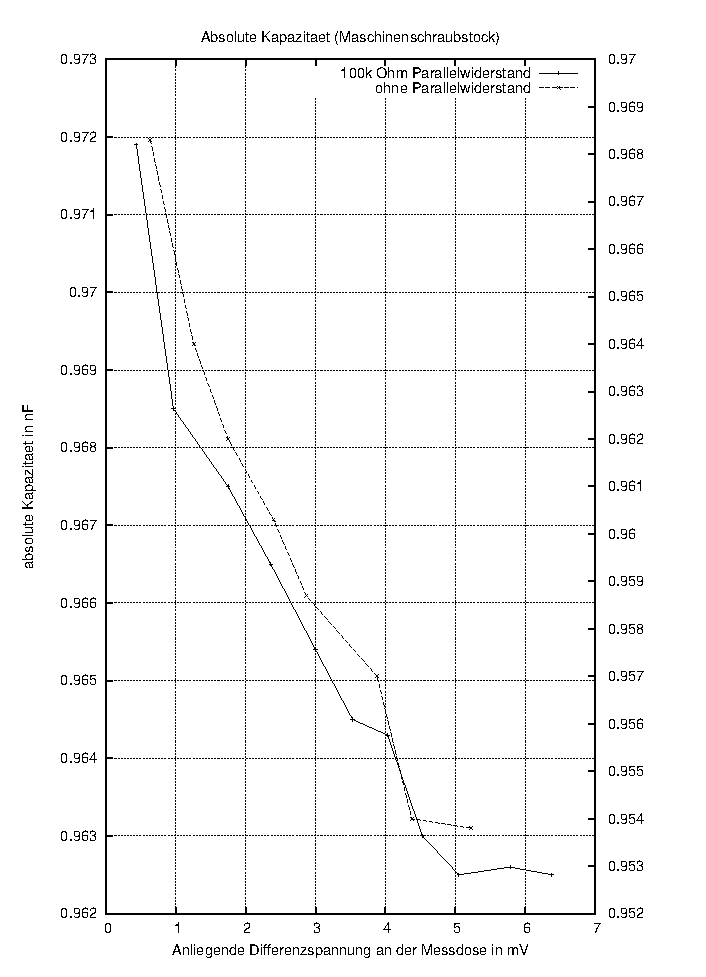
\includegraphics[width=0.8\textwidth-2\fboxsep-2\fboxrule]{tabelle2_1_3}}
      \end{center}
Quelle: Stephan Jobstmann
\label{fig:2.3}
\end{figure}
\newpage
\subsubsection{Messung mit anderer Impedanzmessfrequenz}
Da generell eine Veränderung des Impedanzverhaltens über die Frequenz bei Piezoelementen zu erwarten ist, wurde diese Messung mit halber Frequenz angestrebt. Allerdings sind die sich ergebenden Unterschiede so gering, dass sie von parasitären Effekten überlagert werden und die äußeren Umwelteinflüsse (Temperatur, relative Luftfeuchte) maßgebend für die Ergebnisse sind. Die erzielten Werte sind der Tabelle \vref{tab:2.5} zu entnehmen. Die weiterhin fallende Kapazitätskurve über die Druckbelastung ist in Abbildung \vref{fig:2.4} ersichtlich.\\
Um eine weitere qualitative Aussage über das Frequenzverhalten treffen zu können, wurde empirisch die erste Resonanzfrequenz des Piezoelements ermittelt. Hierzu wurde ein Frequenzgenerator mit manuellem Sweep betrieben und mithilfe eines Shuntwiderstands der Strom in Serie auf Extrema beobachtet. Nach dieser Messung lässt sich ein Resonanzverhalten bei ca. 2.84 MHz feststellen. Aufgrund des weiten Abstands zur Messfrequenz können weitere Schlüsse gezogen werden. Daraus lässt sich auch die unveränderte Charakteristik der vorhergehenden Messung bestätigen.

\setlongtables
\begin{longtable}{| l | l |}
\caption{Messung 5; 1kHz Messfrequenz}\\
\hline
$U_{diff}$ in mV&$C_{Piezo}$ in nF\\
\hline
\endfirsthead
\hline
$U_{diff}$ in mV&$C_{Piezo}$ in nF\\
\hline
\endhead
\hline
\multicolumn{2}{|c|}{Fortsetzung auf der nächsten Seite}\\
\hline
\endfoot
\hline \hline
\endlastfoot
\hline
\label{tab:2.5}%
0.4&0.9705\\
1.4&0.9709\\
2.0&0.9690\\
3.0&0.9681\\
3.8&0.9675\\
5.0&0.9670\\
\end{longtable}

\begin {figure}[htbp]
\caption{Messung 5; 1kHz Messfrequenz}
      \begin{center}
    \fbox{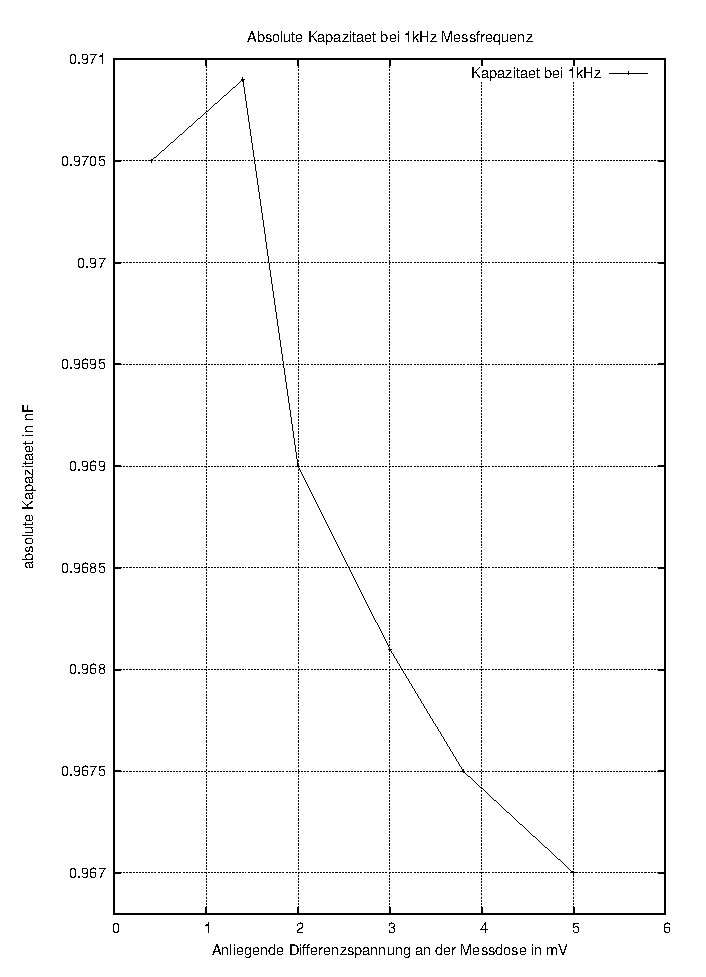
\includegraphics[width=0.8\textwidth-2\fboxsep-2\fboxrule]{tabelle2_1_4}}
      \end{center}
Quelle: Stephan Jobstmann
\label{fig:2.4}
\end{figure}

\newpage
\subsection{Bürklin Piezo-Stack von Elliptec}
Da die vorhergehenden Messungen mit dem einfach aufgebauten Piezoelement nicht die erforderlichen Resultate bezüglich Charakteristik und Reproduzierbarkeit brachten, wurde nun eine Versuchsreihe mit gestapelten Piezoelementen angestrebt. Der Messaufbau blieb weiterhin derselbe, d.h. mithilfe eines Schraubstocks mit Kunststoffbacken wurde eine mechanische Druckbelastung an den Piezostack (im Folgenden auch Stack genannt) und einer Kraftmessdose in Serie angelegt. Beim verwendeten LCR-Meter wurden folgende Parameter eingestellt:
\begin{itemize}
\item 1kHz
\item 1V
\item R.H. off
\item C.V. off
\item int B. off
\end{itemize}
Weiter wurden bei diesen Messungen die Zuleitungen nicht auf dem Stack direkt aufgelötet, da dies den Messvorgang an sich unmöglich gemacht hätte. Stattdessen wurden Keramikträger als lose Verbindung der Messleitungen zum Piezoelement vewendet. Dadurch kann es bei geringer mechanischer Belastung zu Verfälschungen gekommen sein, da der Kontakt zwischen Stack und Keramik unzureichend war.
\subsubsection{Messung Piezo-Stack, ohne Entladungsmaßnahme}
Bei dieser ersten Vermessung des kapazitiven Verhaltens des Piezostacks unter Druckbelastung in elektrischer Feldrichtung wurde eine Entspannungs-Zeit der Kunststoffbacken des Schraubstocks von 2 Minuten berücksichtigt. Es wurde lediglich der Piezo ohne zusätzlichen Parallel- oder Serienwiderstand vermessen. Die auffällig abweichenden Anfangswerte in Abbildung \vref{fig:2.6} sind auf den schlechten Kontakt zwischen Keramikplättchen und Stack bei geringer Druckbelastung zurückzuführen. Die aufgenommenen Werte sind in Tabelle \vref{tab:2.6} zu finden.

\setlongtables
\begin{longtable}{| l |l| l |}
\caption{Messung 6; Piezostack; Einführende Messung}\\
\hline
$U_{diff}$ in mV&$C_{Piezo}$ in nF&$R_{Parallel}$ in k$\Omega$\\
\hline
\endfirsthead
\hline
$U_{diff}$ in mV&$C_{Piezo}$ in nF&$R_{Parallel}$ in k$\Omega$\\
\hline
\endhead
\hline
\multicolumn{3}{|c|}{Fortsetzung auf der nächsten Seite}\\
\hline
\endfoot
\hline \hline
\endlastfoot
\hline
\label{tab:2.6}%
0.7&253.25&2.39\\
1.2&270.00&8.01\\
1.9&271.39&15.48\\
2.9&271.83&16.98\\
3.6&271.98&17.40\\
4.5&272.22&17.42\\
6.1&272.47&15.80\\
7.0&272.70&17.72\\
8.0&272.83&18.28\\
9.4&273.16&18.30\\
10.9&273.62&17.21\\
\end{longtable}

\begin {figure}[htbp]
\caption{Messung 6; Einführende Messung Piezostack}
      \begin{center}
      \fbox{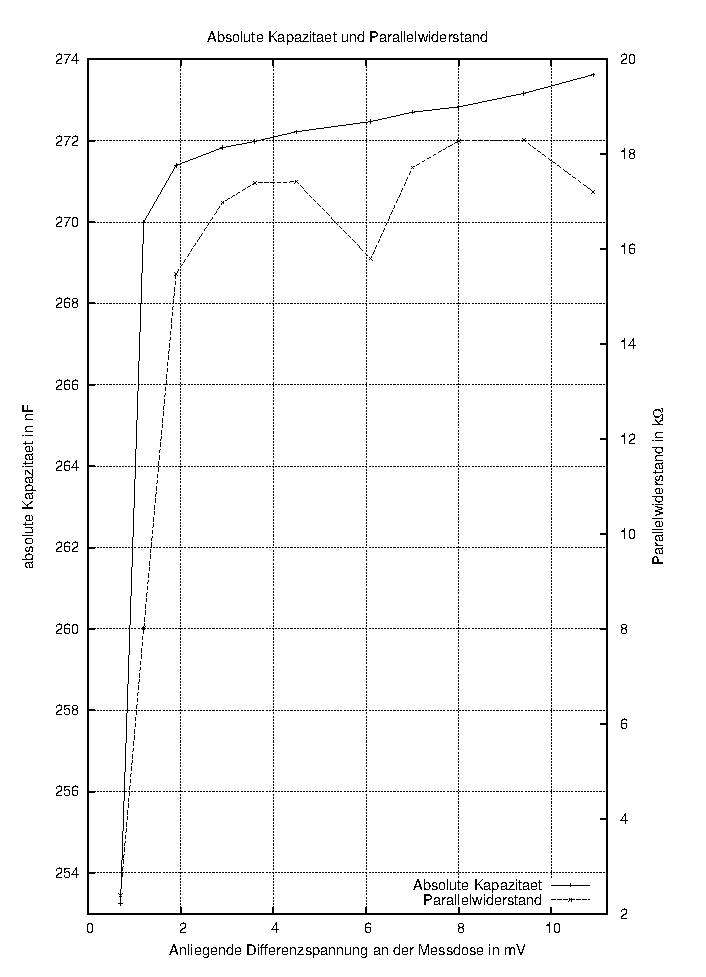
\includegraphics[width=0.8\textwidth-2\fboxsep-2\fboxrule]{tabelle2_2_1}}
      \end{center}
Quelle: Stephan Jobstmann
\label{fig:2.6}
\end{figure}

\newpage
\subsubsection{Messung Piezo-Stack, mit Entladung, ohne Setz-Zeit}
Um störende, vom Stack selbst erzeugte Ladungsquellen ausschließen zu können, wurde diese Messung in jeweils zwei Schritten ausgeführt. Beim ersten Schritt wird die Kraft angelegt und der Piezo-Stack kurzgeschlossen, um so möglicherweise erzeugte Ladungen zu eliminieren. Als zweiten Schritt wird mithilfe des LCR-821 eine Impedanzmessung durchgeführt. Diese beiden Schritte wurden je unter 30 Sekunden durchgeführt, um ein möglichst isochrones Ergebnis zu erhalten. 
Weiter wurde die Messung ein zweites Mal durchgeführt, um eine Aussage über die Reproduzierbarkeit treffen zu können. Beim Vergleich der Graphen in Abbildung \vref{fig:2.7} wird deutlich, dass selbst bei unmittelbar aufeinanderfolgenden Messungen keine zureichende Wiederholbarkeit der Messvorgänge erreicht werden kann. Die korrespondierenden Werte beider Messungen sind in Tabelle \vref{tab:2.7} zu finden.
Um Rückschlüsse auf das $\varepsilon$ des Piezomaterials zu ermöglichen, wurde der Parallelwiderstand bei diesem Messvorgang mit aufgezeichnet. Die Resultate sind in der Tabelle \vref{tab:2.8} und Abbildung \vref{fig:2.8} ersichtlich.

\setlongtables
\begin{longtable}{| l | l | l | l |}
\caption[Messung 7; ohne Setz-Zeit; Kapazität]{Messung 7; Piezostack; mit Entladung, ohne Setz-Zeit; Kapazität}\\
\hline
\multicolumn{2}{|c|}{Messung 1} &\multicolumn{2}{|c|}{Messung 2}\\
\hline
$U_{diff}$ in mV&$C_{Piezo}$ in nF&$U_{diff}$ in mV&$C_{Piezo}$ in nF\\
\hline
\endfirsthead
\hline
\multicolumn{2}{|c|}{Messung 1} &\multicolumn{2}{|c|}{Messung 2}\\
\hline
$U_{diff}$ in mV&$C_{Piezo}$ in nF&$U_{diff}$ in mV&$C_{Piezo}$ in nF\\
\hline
\endhead
\hline
\multicolumn{4}{|c|}{Fortsetzung auf der nächsten Seite}\\
\hline
\endfoot
\hline \hline
\endlastfoot
\hline
\label{tab:2.7}%
0.15&266.66&0.49&269.02\\
1.15&267.14&1.55&268.98\\
2.55&267.72&2.82&269.26\\
3.24&267.93&3.63&269.36\\
4.39&268.6&4.60&269.55\\
5.10&268.88&5.57&269.78\\
6.14&269.32&6.39&269.90\\
7.55&268.95&7.74&270.25\\
8.24&270.16&8.40&270.40\\
9.82&270.71&9.52&270.70\\
10.45&270.76&10.49&270.84\\
\end{longtable}

\begin {figure}[htbp]
\caption{Messung 7; mit Entladung, ohne Setz-Zeit; Piezostack; Kapazität}
      \begin{center}
     \fbox{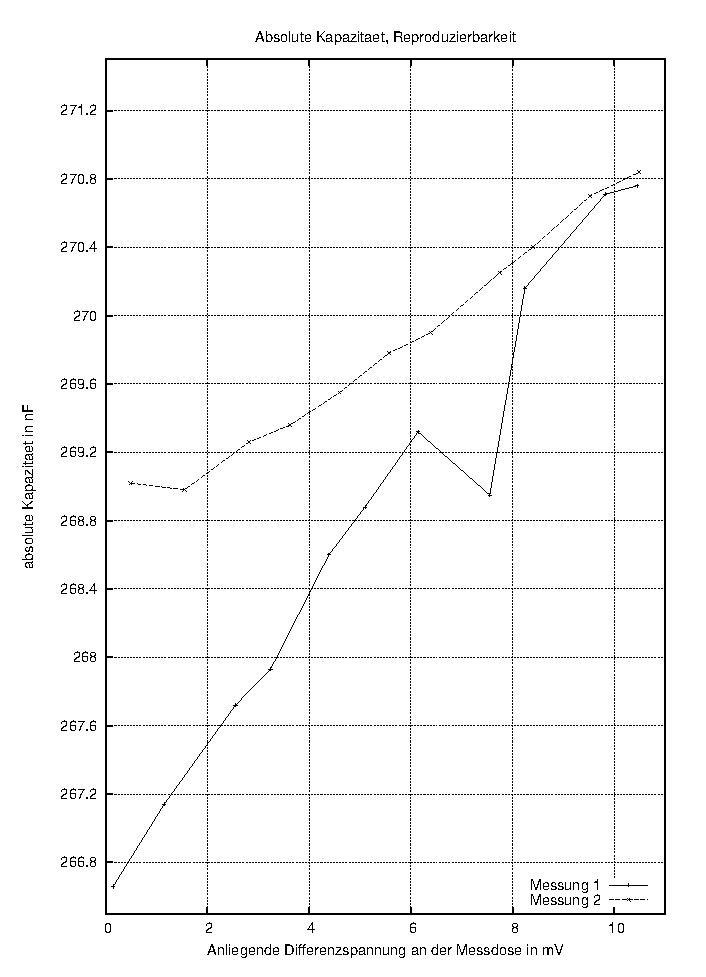
\includegraphics[width=0.8\textwidth-2\fboxsep-2\fboxrule]{tabelle2_2_2}}
      \end{center}
Quelle: Stephan Jobstmann
\label{fig:2.7}
\end{figure}

\setlongtables
\begin{longtable}{| l | l | l | l |}
\caption[Messung 8; ohne Setz-Zeit; Parallelwiderstand]{Messung 8; Piezostack; mit Entladung, ohne Setz-Zeit; Parallelwiderstand}\\
\hline
\multicolumn{2}{|c|}{Messung 1} &\multicolumn{2}{|c|}{Messung 2}\\
\hline
$U_{diff}$ in mV&$R_{Parallel}$ in k$\Omega$&$U_{diff}$ in mV&$R_{Parallel}$ in k$\Omega$\\
\hline
\endfirsthead
\hline
\multicolumn{2}{|c|}{Messung 1} &\multicolumn{2}{|c|}{Messung 2}\\
\hline
$U_{diff}$ in mV&$R_{Parallel}$ in k$\Omega$&$U_{diff}$ in mV&$R_{Parallel}$ in k$\Omega$\\
\hline
\endhead
\hline
\multicolumn{4}{|c|}{Fortsetzung auf der nächsten Seite}\\
\hline
\endfoot
\hline \hline
\endlastfoot
\hline
\label{tab:2.8}%
0.15&16.53&0.49&17.42\\
1.15&19.24&1.55&18.38\\
2.55&19.25&2.82&18.68\\
3.24&19.58&3.63&18.63\\
4.39&19.19&4.60&18.72\\
5.10&19.15&5.57&17.72\\
6.14&18.93&6.39&18.70\\
7.55&18.62&7.74&18.65\\
8.24&18.58&8.40&17.63\\
9.82&18.38&9.52&18.55\\
10.45&18.51&10.49&18.60\\
\end{longtable}

\begin {figure}[htbp]
\caption[Messung 8; ohne Setz-Zeit; Parallelwiderstand]{Messung 8; Piezostack; mit Entladung, ohne Setz-Zeit; Parallelwiderstand}
      \begin{center}
       \fbox{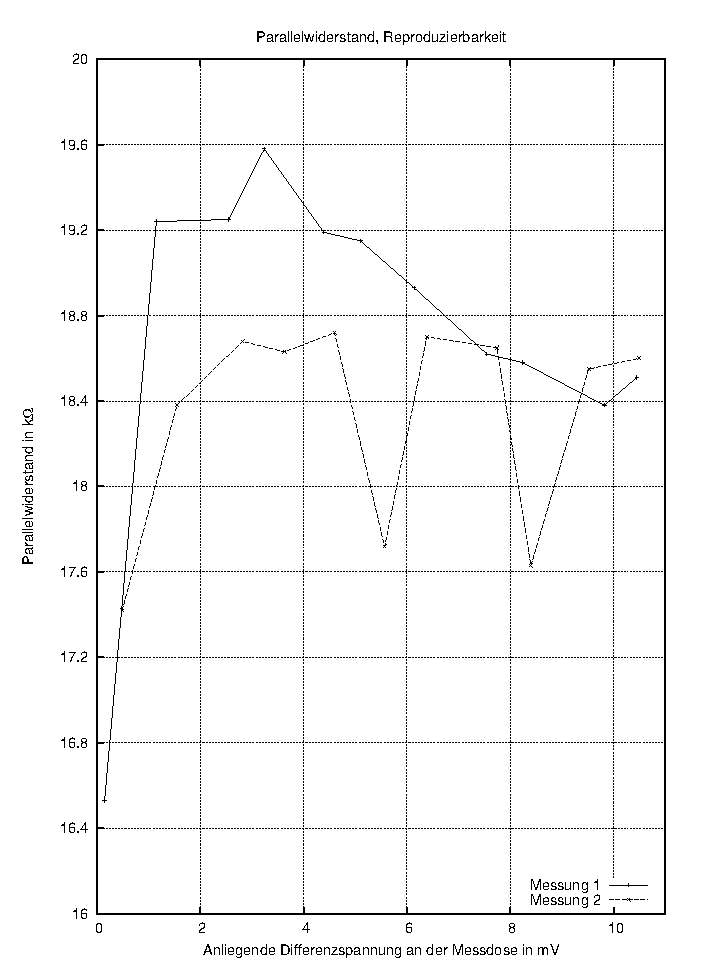
\includegraphics[width=0.8\textwidth-2\fboxsep-2\fboxrule]{tabelle2_2_3}}
      \end{center}
Quelle: Stephan Jobstmann
\label{fig:2.8}
\end{figure}

\newpage
\subsubsection{Messung Piezo-Stack, mit Entladung, mit 2 Minuten Setz-Zeit}
Um eine treffen Aussage fassen zu können, wurde die vorhergehende Messung komplett wiederholt. Jedoch wurde dieses mal bei den einzelnen Werten eine Setz-Zeit von 2 Minuten eingehalten, um etwaige Fehler aufgrund des elastischen Materials der Schraubstockbacken zu minimieren. Allerdings sind auch hier anhand von Abbildung \vref{fig:2.9} die deutliche Abweichung zwischen den Kapazitätslinien zu sehen. Die dazugehörigen Werte sind in Tabelle \vref{tab:2.9} zu finden.\\
Auch hier wurde eine Messung des auftretenden Parallelwiderstands angestoßen. Die Resultate sind in Tabelle \vref{tab:2.10} und Abbildung \vref{fig:2.10} nachzulesen.

\setlongtables
\begin{longtable}{| l | l | l | l |}
\caption[Messung 9; 2 Minuten Setz-Zeit; Piezostack; Kapazität]{Messung 9; Piezostack; mit Entladung, 2 Minuten Setz-Zeit; Kapazität}\\
\hline
\multicolumn{2}{|c|}{Messung 1} &\multicolumn{2}{|c|}{Messung 2}\\
\hline
$U_{diff}$ in mV&$C_{Piezo}$ in nF&$U_{diff}$ in mV&$C_{Piezo}$ in nF\\
\hline
\endfirsthead
\hline
\multicolumn{2}{|c|}{Messung 1} &\multicolumn{2}{|c|}{Messung 2}\\
\hline
$U_{diff}$ in mV&$C_{Piezo}$ in nF&$U_{diff}$ in mV&$C_{Piezo}$ in nF\\
\hline
\endhead
\hline
\multicolumn{4}{|c|}{Fortsetzung auf der nächsten Seite}\\
\hline
\endfoot
\hline \hline
\endlastfoot
\hline
\label{tab:2.9}%
0.55&268.80&1.16&268.90\\
1.17&268.55&2.33&269.23\\
2.26&268.73&3.34&269.35\\
3.27&268.94&4.33&269.43\\
4.27&269.13&4.99&269.51\\
4.93&269.14&6.20&269.85\\
6.10&269.37&7.03&269.90\\
6.95&269.50&8.32&270.30\\
8.21&269.70&9.31&269.99\\
9.24&269.60&10.41&270.33\\
10.30&269.83&&\\
\end{longtable}

\begin {figure}[htbp]
\caption[Messung 9; 2 Minuten Setz-Zeit; Piezostack; Kapazität]{Messung 9; mit Entladung, 2 Minuten Setz-Zeit; Piezostack; Kapazität}
      \begin{center}
        \fbox{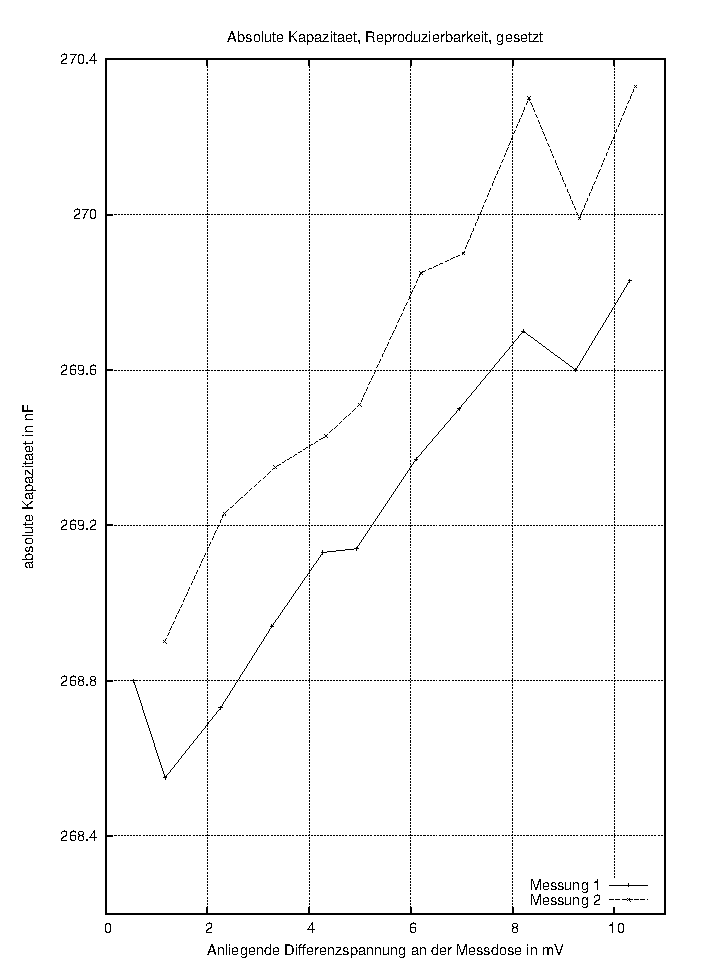
\includegraphics[width=0.8\textwidth-2\fboxsep-2\fboxrule]{tabelle2_2_4}}
      \end{center}
Quelle: Stephan Jobstmann
\label{fig:2.9}
\end{figure}
\setlongtables
\begin{longtable}{| l | l | l | l |}
\caption[Messung 10; 2 Minuten Setz-Zeit; Piezostack; Parallelwiderstand]{Messung 10; Piezostack; mit Entladung, 2 Minuten Setz-Zeit; Parallelwiderstand}\\
\hline
\multicolumn{2}{|c|}{Messung 1} &\multicolumn{2}{|c|}{Messung 2}\\
\hline
$U_{diff}$ in mV&$R_{Parallel}$ in k$\Omega$&$U_{diff}$ in mV&$R_{Parallel}$ in k$\Omega$\\
\hline
\endfirsthead
\hline
\multicolumn{2}{|c|}{Messung 1} &\multicolumn{2}{|c|}{Messung 2}\\
\hline
$U_{diff}$ in mV&$R_{Parallel}$ in k$\Omega$&$U_{diff}$ in mV&$R_{Parallel}$ in k$\Omega$\\
\hline
\endhead
\hline
\multicolumn{4}{|c|}{Fortsetzung auf der nächsten Seite}\\
\hline
\endfoot
\hline \hline
\endlastfoot
\hline
\label{tab:2.10}%
0.55&17.38&1.16&17.80\\
1.17&18.08&2.33&18.65\\
2.26&19.07&3.34&18.80\\
3.27&19.15&4.33&18.88\\
4.27&19.18&4.99&18.89\\
4.93&19.30&6.20&18.87\\
6.10&19.29&7.03&18.69\\
6.95&19.30&8.32&18.82\\
8.21&19.29&9.31&19.10\\
9.24&19.44&10.41&19.00\\
10.30&19.49&&\\
\end{longtable}

\begin {figure}[htbp]
\caption[Messung 10; 2 Minuten Setz-Zeit; Piezostack; Parallelwiderstand]{Messung 10; mit Entladung, 2 Minuten Setz-Zeit; Piezostack; Parallelwiderstand}
      \begin{center}
       \fbox{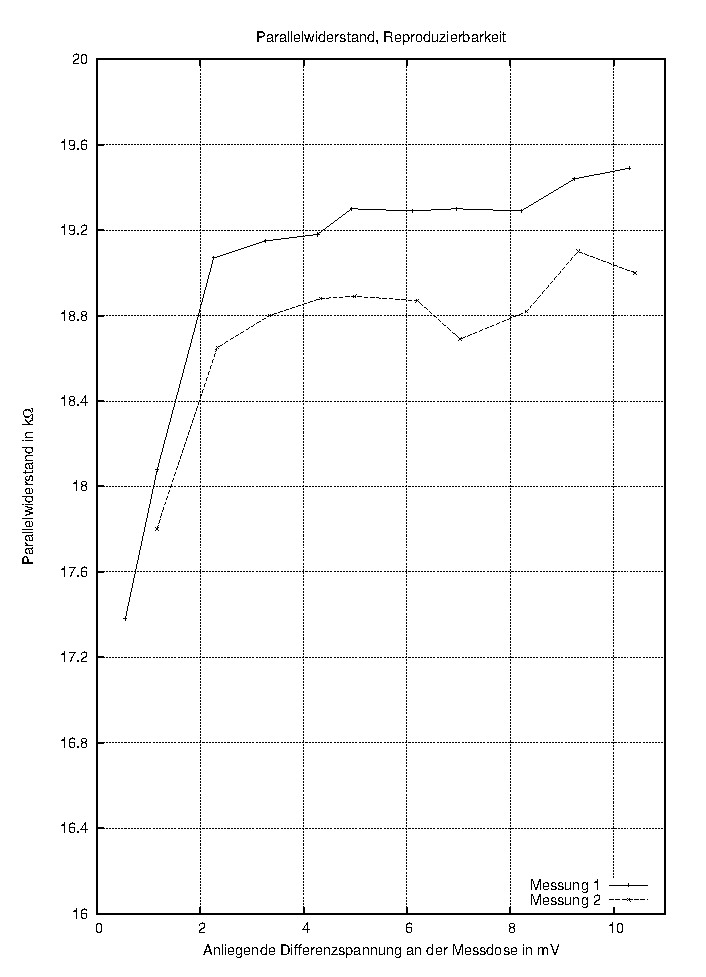
\includegraphics[width=0.8\textwidth-2\fboxsep-2\fboxrule]{tabelle2_2_5}}
      \end{center}
Quelle: Stephan Jobstmann
\label{fig:2.10}
\end{figure}
%
\chapter{Hardware}
Im Folgenden werden die Fortschritte in der Hardware-Entwicklung chronologisch geordnet und in Teilbereiche separiert aufgeführt.
\section{Energiezuführung}
Als zielführend erweist sich eine Vorüberlegung im Bezug auf die Möglichkeiten der elektrischen Speisung. Grundlegende Anforderungen waren hier die Verwendung in hermetisch isolierten Systemen und die Effizienz. Somit ist beispielsweise von vornherein eine direkte Kopplung an eine Netzversorgungsquelle oder eine Speisung durch wechselbare Batterien ausgeschlossen. 
\subsection{Energy-Harvesting}
\label{energy}
In diesem Teilbereich werden zwei physikalische Grundarten des Micro Energy Harvesting betrachtet. Diese sind die Umwandlung von mechanischer Schwingungsenergie und thermischer Differenz in elektrische Spannung. Bei der Vorbereitung und Einarbeitung in die entsprechende Thematik wird bei der Umformung von mechanischen Schwingungen in Elektrizität offensichtlich, dass dies eine ungünstige Form der Energiegewinnung für dieses System ist. Dies liegt unter anderem an der unmöglichen Abstimmung der durch den Auftritt erzeugten Erregung auf die Resonanzfrequenz des Schwingungsaufnehmers. Weiter benötigt ein solches Bauelement einen Freiraum um seine abklingende Bewegung harmonisch abbauen zu können. Es müssen auch die maximal auftretenden Beschleunigungen berücksichtigt werden was wiederum zu einer Versteifung des kompletten Federsystems führen würde. Das hätte als Resultat, dass durch die Erhöhung der dynamischen Bandbreite die verhältnismäßig kleineren Anregungen einen schlechteren Wirkungsgrad liefern würden. Diese Umstände schließen die piezoelektrische Wandlung leider für die Option der Energiezuführung aus. \citep[vgl. S.39]{Dembowski2011} \newline 
Die thermoelektrische Wandlung beruht auf der Inversen des Peltier-Effekts, dem Seebeck Effekt. Diesem liegt zu Grunde, dass am Übergang von zwei unterschiedlichen Metallen unterschiedlicher Temperierung ein elektrisches Feld aufgebaut wird. Die Verwendung dieses Effekts war zunächst nur bei Temperatur-Messfühlern weit verbreitet. Allerdings ist aufgrund der fortschreitenden Entwicklung der Micro Energy Harvesting Technologien dieser Effekt mittlerweile auch zur Energieversorgung nutzbar. \newline \newline
Als zentralen Baustein für die Erprobung von Micro-Energy-Harvesting Systemen im Bezug auf thermo-elektrische Energiewandlung bietet sich der \textit{LTC3108} von der Firma Linear Technology an. Dieser vermag mit geringem Aufwand Eingangsspannungen von 20mV bis 500mV auf ausgangsseitig bis zu 5V aufwärts zu wandeln. Um möglichst schnell Erkenntnisse aus der Wirkungsweise des Bausteins ziehen zu können, wird eine im Internet veröffentlichte Schaltung\footnote{Github Repository of wa7iut \citep{git}} für Tests verwendet (siehe Abbildung \vref{fig:4.1}). Diese hält sich strikt an die Vorgaben des Datenblatts\footnote{LTC3108 - Ultralow voltage Step-Up Converter and Power Manager \citep{LTC}} \citep{LTC3108}. Beim LTC3108 handelt es sich um einen Spannungs-Aufwärtswandler\footnote{Step-Up-Converter} für sehr niedrige Eingangsspannungen. Im Gegensatz zum normalen Aufbau von Aufwärtswandlern wird keine einfache Induktivität sondern ein kleiner Transformator verwendet. Dies reduziert zwar aufgrund des hohen Übersetzungsverhältnisses (1:20 bis 1:100) den Wirkungsgrad, allerdings lassen sich so auch höhere Spannungen erzeugen. Bei dem Versuchsaufbau wird ein 1:100 Transformator verwendet, da sich die Eingangsspannungen, welche experimentell ermittelt wurden, sich zwischen 20mV und 90mV bewegen. Als zu erstrebende Ausgangsspannung wurde schaltungstechnisch 3,3V eingestellt, da dies die zur Zeit am häufigsten bei Mikrocontrollern vorkommende Versorgungsspannung ist. Als externer Energiespeicher wurde ausgangsseitig an die Schaltung ein $2200 \mu$F Kondensator angefügt. Als energieerzeugendes Element wurde ein Peltierelement mit einem Aluminium-Kühlkörper versehen. So muss bei ausreichender zugeführter Wärme nicht einmal aktiv gekühlt werden, es genügt die Wärmeveräußerung durch den Kühlkörper.%weitere Fotos
\begin{figure}[htb]
\caption{LTC3108 Board von Ambient Sensors}
\centering
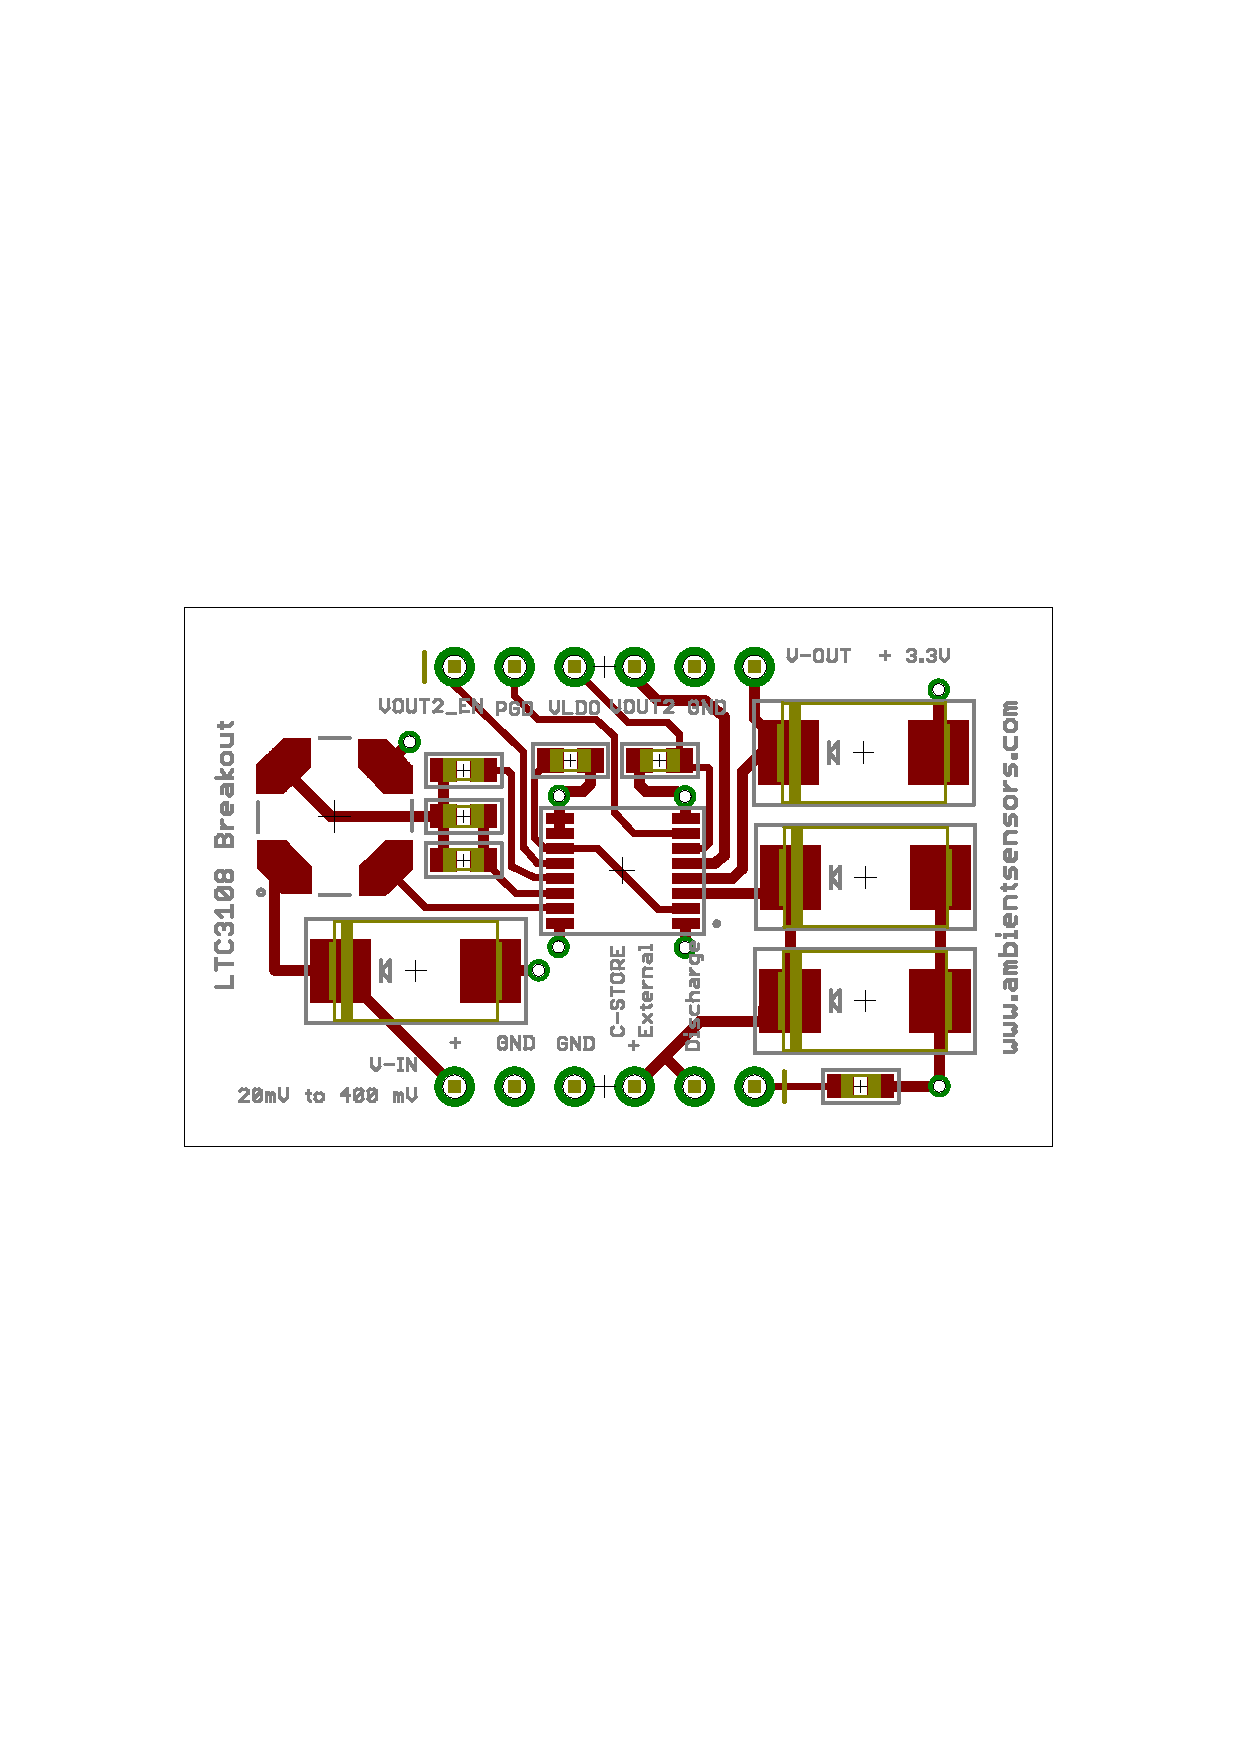
\includegraphics[bb=3.4cm 10.6cm 17.5cm 19.4cm]{Bilder/LTC3108breakoutSSOC}
\\Quelle: Stephan Jobstmann
\label{fig:4.1}
\end{figure}
\subsection{Drahtlose Energieübertragung}
\label{chap:4.1.2}
Zum Laden der internen Speicher, die in Kapitel \vref{chap:4.2} vorgestellt werden, wird eine vielfach höhere Leistung benötigt als jene, die mit den Mitteln des Energy-Harvesting bereitgestellt werden kann. Allerdings sollen bei die durch die Grundvoraussetzung festgelegten Richtlinien nicht verletzt werden. Durch den betreuenden Professor Harasim kam die Vorgabe ein Evaluations-Kit der Firma Texas Instruments genauer zu untersuchen. Dabei handelte es sich um ein System, welches aus zwei Komponenten bestand:
\begin{itemize}
\item
Transmitter, Sender: bq500110EVM-688 Evaluation Module (Abbildung \ref{BQ_transm})
\item
Receiver, Empfänger: bq51013EVM-725 Evaluation Module (Abbildung \ref{BQ_rec})
\end{itemize}
\begin{figure}
\caption{Transmitter-Modul des Evaluation-Packs}
\centering
\fbox{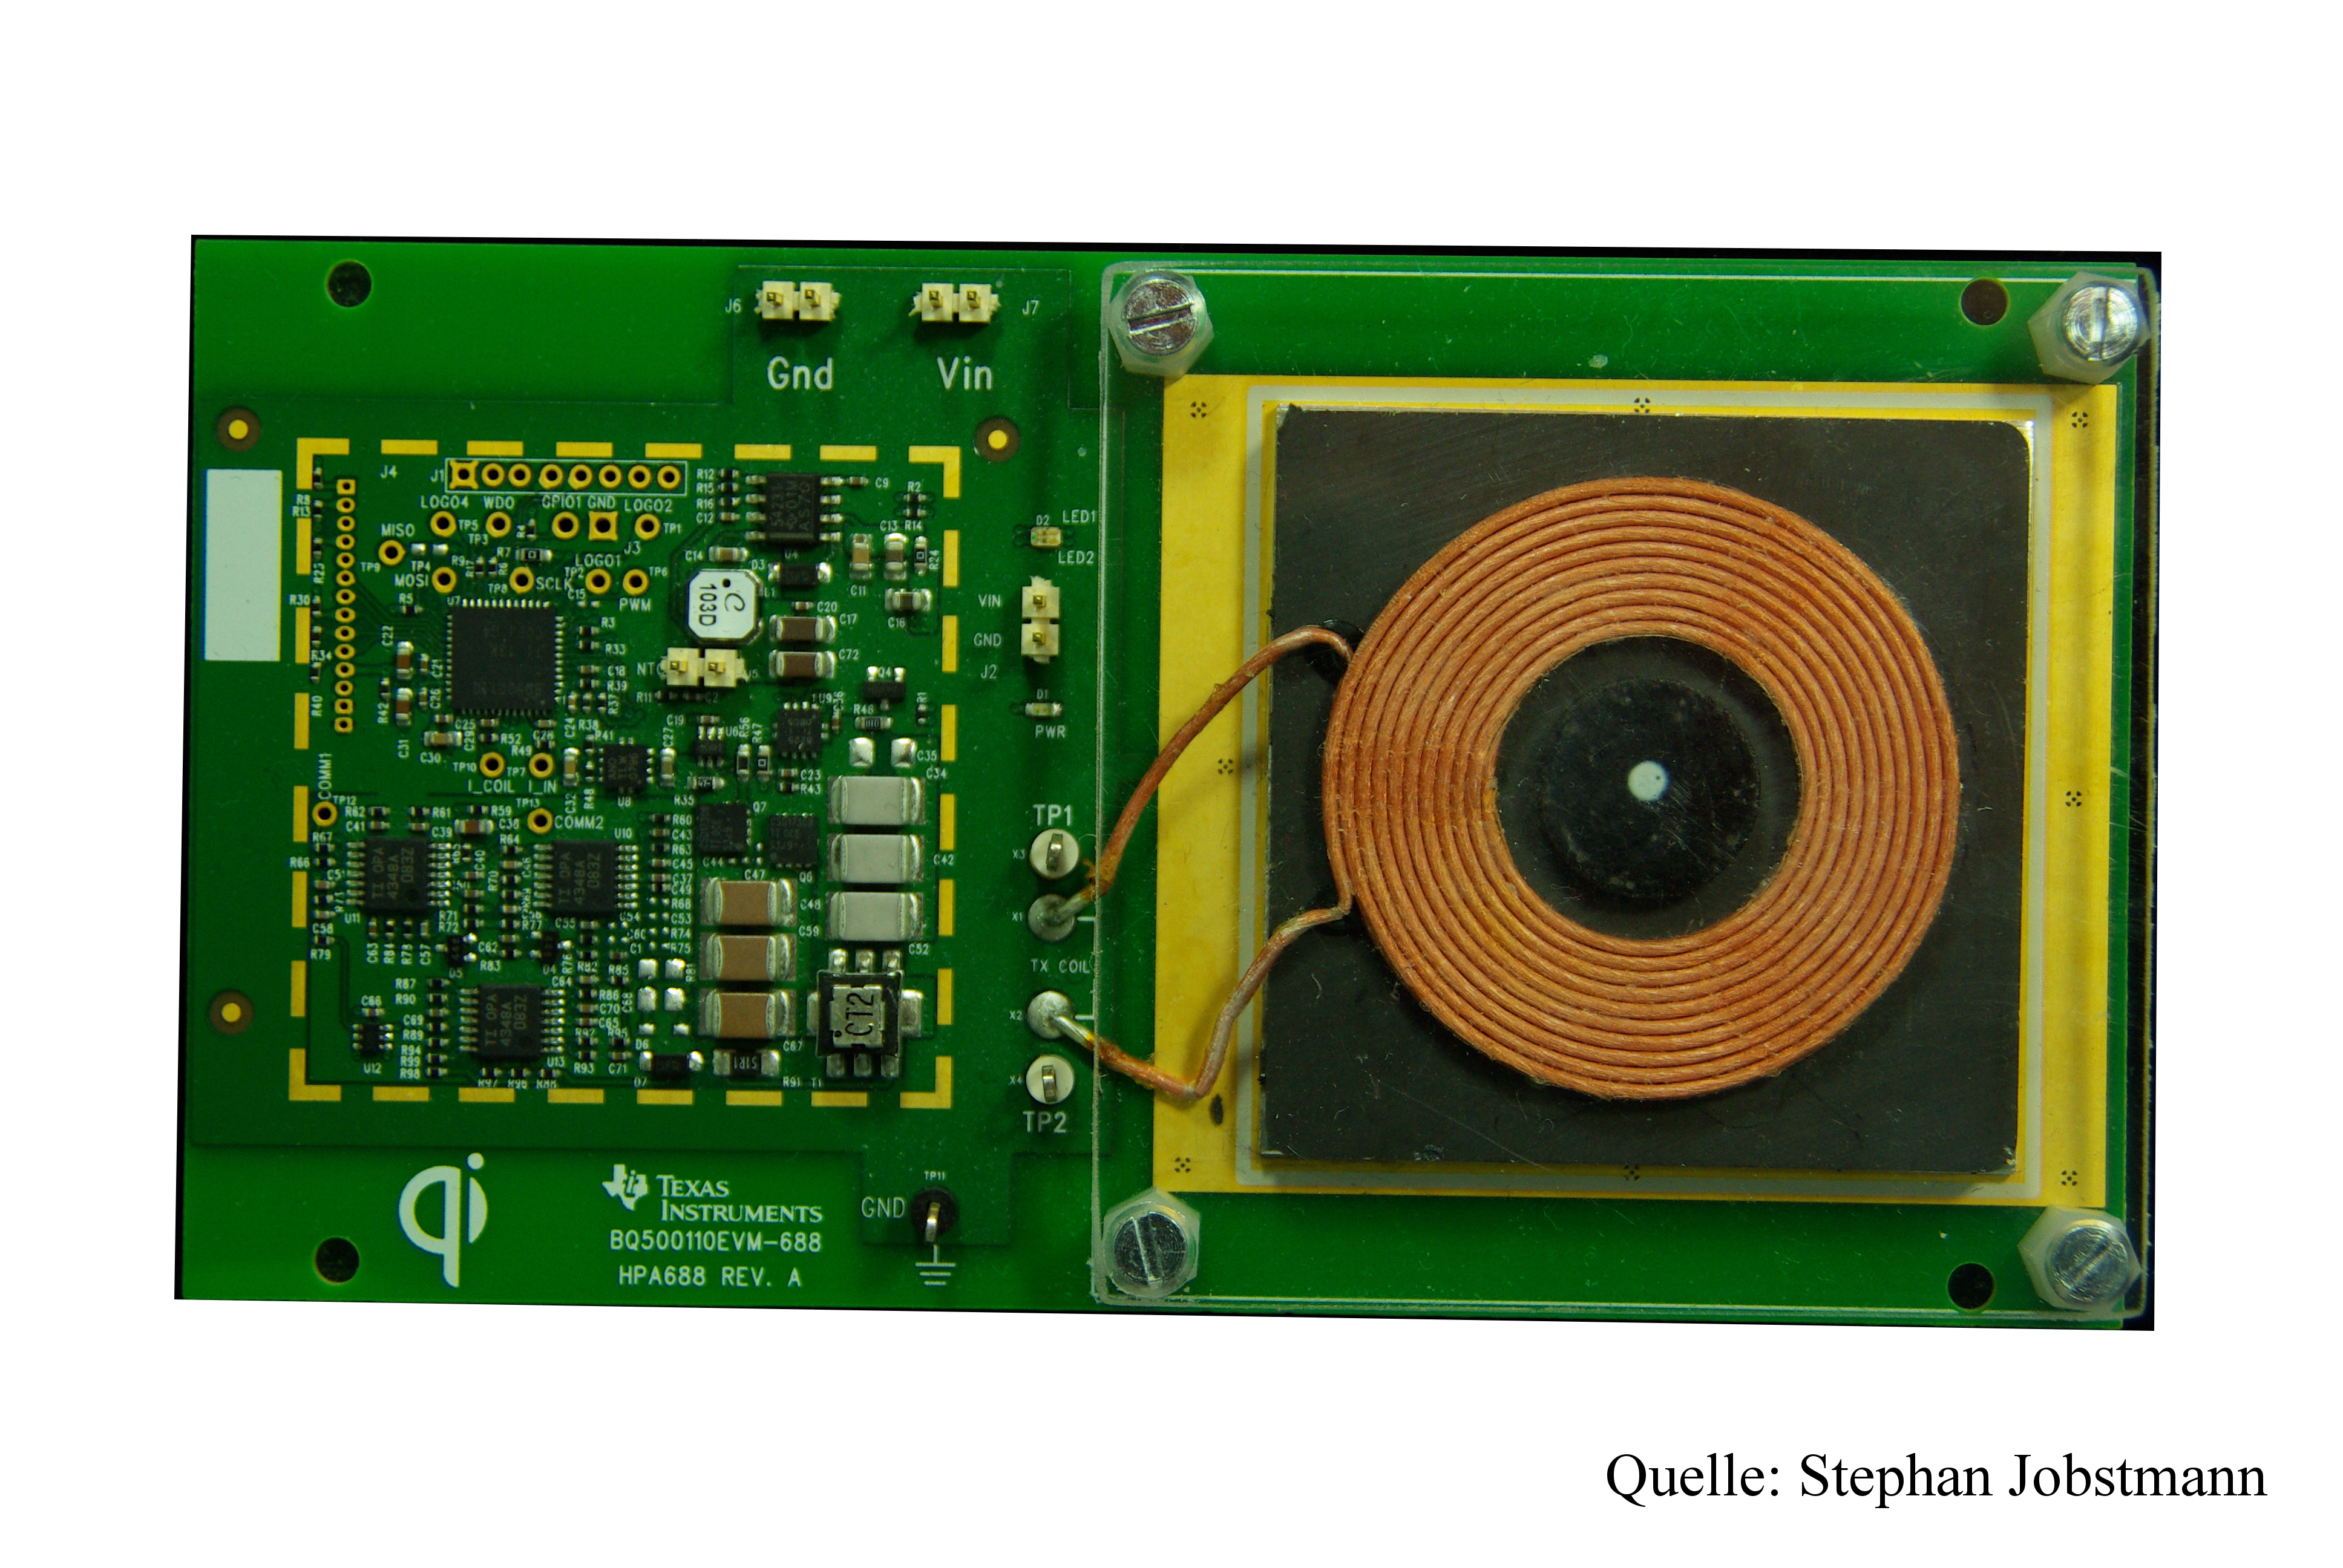
\includegraphics[width=0.8\textwidth-2\fboxsep-2\fboxrule]{Bilder/BQ_Tesla_transmitter.JPG}}
\\Quelle: Stephan Jobstmann
\label{BQ_transm}
\end{figure}
\begin{figure}
\centering
\caption{Receiver-Modul des Evaluation-Packs}
\fbox{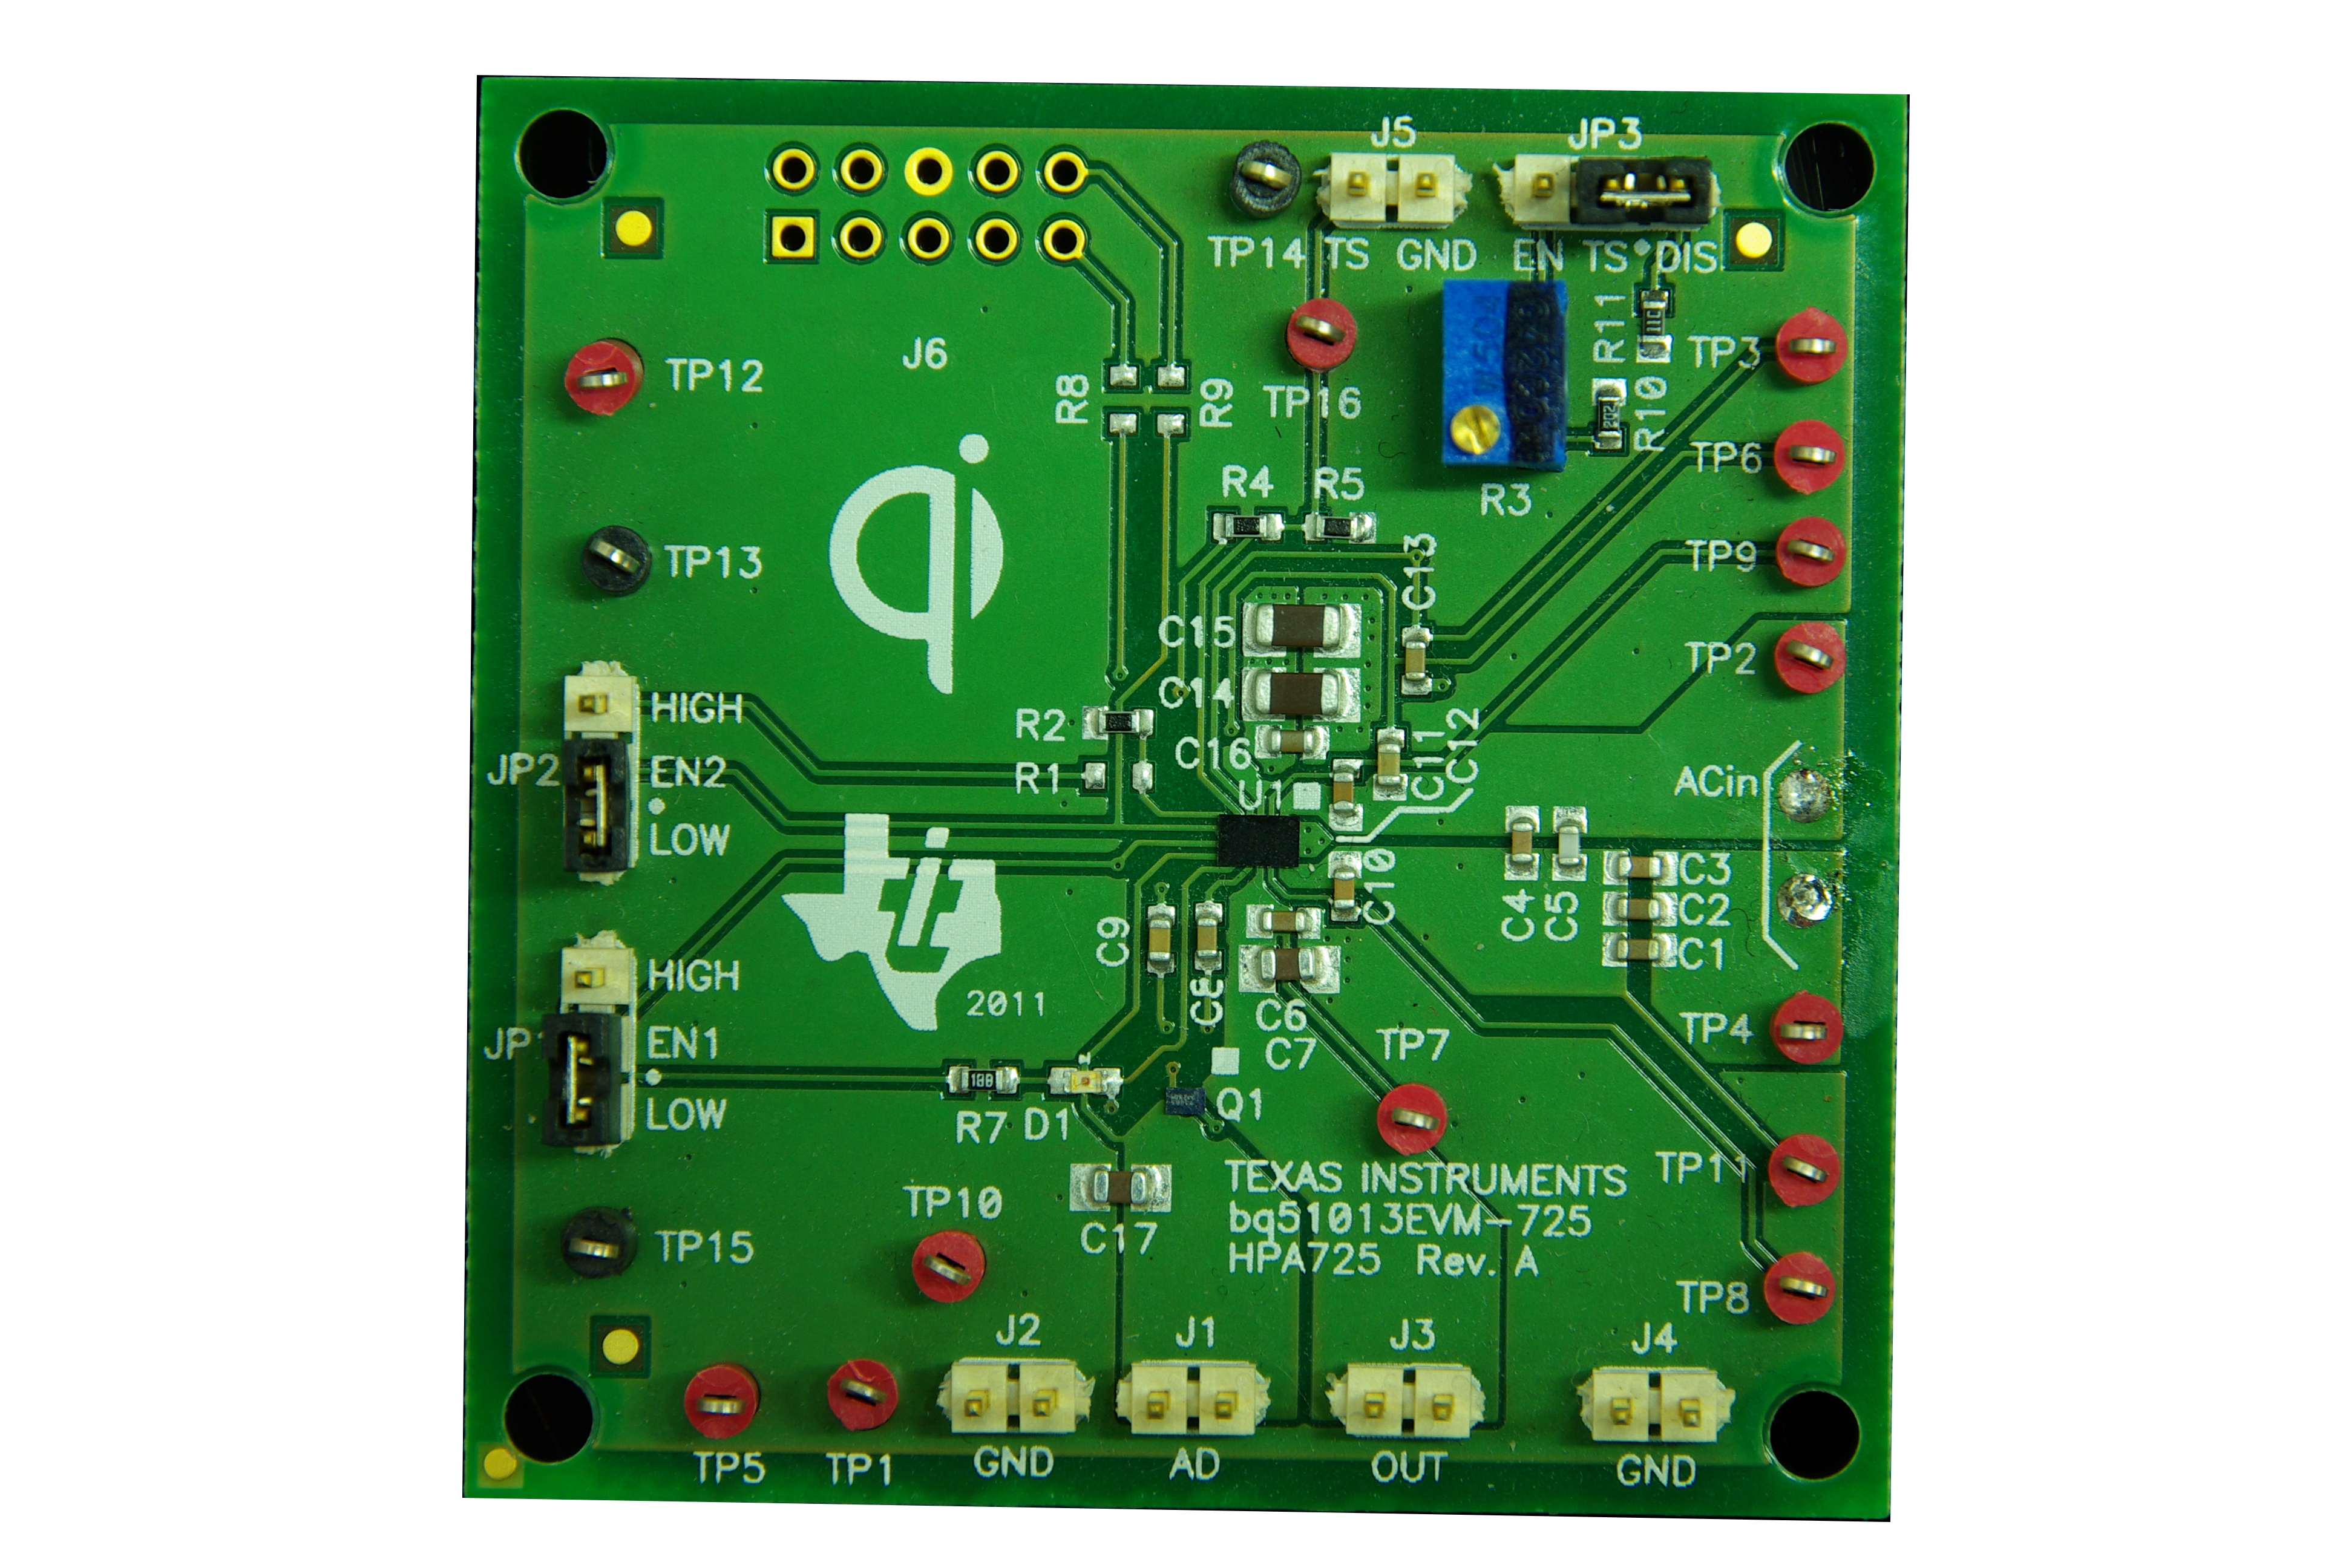
\includegraphics[width=0.8\textwidth-2\fboxsep-2\fboxrule]{Bilder/BQ_Tesla_receiver.JPG}}
\\Quelle: Stephan Jobstmann
\label{BQ_rec}
\end{figure}
Dieses lässt sich mithilfe einer Gleichspannungsquelle, eingestellt auf eine Speisung von 19V und einer Stromgrenze über 0,5A sehr einfach in Betrieb nehmen. Am Empfängermodul stellt sich bei passgenauer Platzierung der beiden Übertragerspulen des magnetischen Kopplungssystems eine Tätigkeit der Indikationsanzeige ein. Ein Permanentmagnet hilft beim Zentrieren der beiden Luftspulen. Laut Datenblatt \citep[vgl. S.2]{bq51013EVM-725} liefert die Beispielschaltung 5V bei 1A. Zum Testen der Kompatibilität wurde die Schaltung mit der in Kapitel \ref{chap:4.2.2} vorgestellten Ladeeinheit gekoppelt. Das erfolgreiche Zusammenarbeiten konnte reproduzierbar getestet werden.\\
Für das Gesamtkonzept des Fußmoduls vom Projekt "`MedLast"' ist die Empfangseinheit vorrangig. Um eine passendes Zusammenspiel von proprietärer Sendeeinheit und selbstentworfener Empfangsschaltung sicherzustellen, wurde der gleiche Baustein (\textit{BQ51013}) verwendet. Allerdings wurde beim Schaltungsaufbau darauf geachtet, dass der Bauteilumfang sich auf ein Minimum reduziert. So wurde die Zusatzbeschaltung für eine eventuelle alternative bedrahtete Versorgung weggelassen. Bei dem BQ51013 handelt es sich um ein IC, welches nur in BGA\footnote{Ball Grid Array} Gehäusegröße erhältlich ist. Da dies wiederum für das Layoutdesign bedeutete, dass mit Kontaktflächengrößen von $250\mu$m gearbeitet werden muss, ergab sich eine weitere Problematik. Die typischen Leiterplattenhersteller für Prototypen und Kleinserien haben eine Vorgabe für den Mindestdurchmesser von Durchkontaktierungen mit $300\mu$m. D.h. über die üblichen Wege war es nicht ohne Mehraufwand möglich, einen Platine zu beschaffen. Da ein Durchmesser der Durchkontaktierungen von $150\mu$m als maximale Maßgabe anzusehen war, wurde für den Prototypenbau LTCC\footnote{Low Temperature Cofire Ceramic} als Schaltungsträger ausgewählt. Diese können im Hybridlabor in Dickschichttechnik selbstständig aufgebaut werden. Weiter können durch das Laserstruktur-Gerät \textit{ProtoLaser U} die Keramiksubstrate auf $15\mu$m genau geritzt und gebohrt werden.  Da LTCC im einlagigen Aufbau zu fragil wäre, wurden noch Überlegungen angestrebt um die mechanische Widerstandsfähigkeit zu erhöhen. Ein mehrlagiger Aufbau barg eine zu große Gefahr im Bezug auf die erhöhte Wahrscheinlichkeit einer unterbrochenen Durchkontaktierung. Diese steigt proportional mit der Anzahl der verwendeten Lagen LTCC. Durch einen Hinweis von Herrn Leschik wurde bei einem zweiten Versuch die LTCC-Schicht, welche den beidseitigen Schaltungsdruck aufgetragen hatte, auf eine $Al_2O_3$-Keramik auflaminiert. Diese dient als mechanisch-stabiler Träger. Nach einem ersten Fehlversuch konnten somit auf einem Substrat mit Mehrfach-Nutzen mehrere, passiv einwandfreie Schaltungen aufgebaut werden. Nach deren Bestückung per Hand und Lötung mit der Dampfphasenanlage der Hochschule Landshut wurde diese mit der Einkopplungsspule verbunden. Eine anfängliche Überlegung, diese ebenfalls auf Dickschichttechnik basierend auf LTCC zu der Schaltung zu bringen, wurde aufgrund der nicht einzuhaltenden Kriterien an die Güte der Induktivität wieder verworfen. Darum fiel die Entscheidung auf eine Empfänger-Spule, welche von der Firma Würth Elektronik genau für diesen Zweck bereitgestellt wird \citep{Spule}. Die für den Empfängerschwingkreis noch benötigten Kapazitäten wurden über folgende Formeln des Datenblatts \citep{BQ51013} dimensioniert: 
\begin{eqnarray}
C1&=&\left[\left(f_S \cdot 2\pi\right)^2 \cdot L'_S\right]^{-1}\\
C1&=&\left[\left(100\text{kHz} \cdot 2\pi\right)^2 \cdot 0,01011\text{mH}\right]^{-1}\\
C1&=&250\text{nF}\\
\nonumber\\
C2&=&\left[\left(f_D \cdot 2\pi\right)^2 \cdot L_S-\frac 1{C1}\right]^{-1}\\
\nonumber\\
C2&=&\left[\left(1\text{MHz} \cdot 2\pi\right)^2 \cdot 0,01011\text{mH}-\frac 1{250\text{nF}}\right]^{-1}\\
\nonumber\\
C2&=&2,53\text{nF}\\
\nonumber\\
Q&=&\frac{2\pi \cdot f_D \cdot L_S}{R}\\
\nonumber\\
Q&=&\frac{2\pi \cdot 1\text{MHz} \cdot 0,01011\text{mH}}{0,1488 \Omega}\\
\nonumber\\
Q&=&426,90
\end{eqnarray}
Als Mindestmaß wird im Datenblatt \citep[siehe S.23]{BQ51013} eine Güte von 77 festgelegt. Diese wird mit der Luftspule von Würth Elektronik weit überschritten.\\
Mit drei, beziehungsweise zwei diskreten Kondensatoren wurden die Kapazitäten $C1$ und $C2$ aufgebaut. Dies wurde auf einer separaten, zwischen Spule und Keramikschaltung gelöteten Platine aufgebaut. Der fertige selbstentworfene Aufbau wurde mit einer geringen Last von $47 \Omega$ auf die von Texas Instruments bereitgestellte Schaltung\footnote{bq500110EVM-688, Sendeeinheit} gesetzt und getestet. Dieser ist auf Grafik \vref{self_rec} zu sehen. Die Reproduzierbarkeit wies noch Defizite auf, so konnte noch nicht sichergestellt werden, dass bei jedem Aufsetzen der Empfängerschaltung eine stabile Verbindung zustande kommt. Weiter können noch keine niederohmigen Lasten ($<50 \Omega$) an das Modul gekoppelt werden. Dies mag zum ein an der unzureichenden Anpassung des Schwingkreises liegen oder auch zum anderen an der Hochohmigkeit der gedruckten Leiterbahnen auf dem Keramiksubstrat. 
\begin{figure}
\centering
\caption{Receiver-Modul, hergestellt im Hybridlabor der Hochschule Landshut}
\fbox{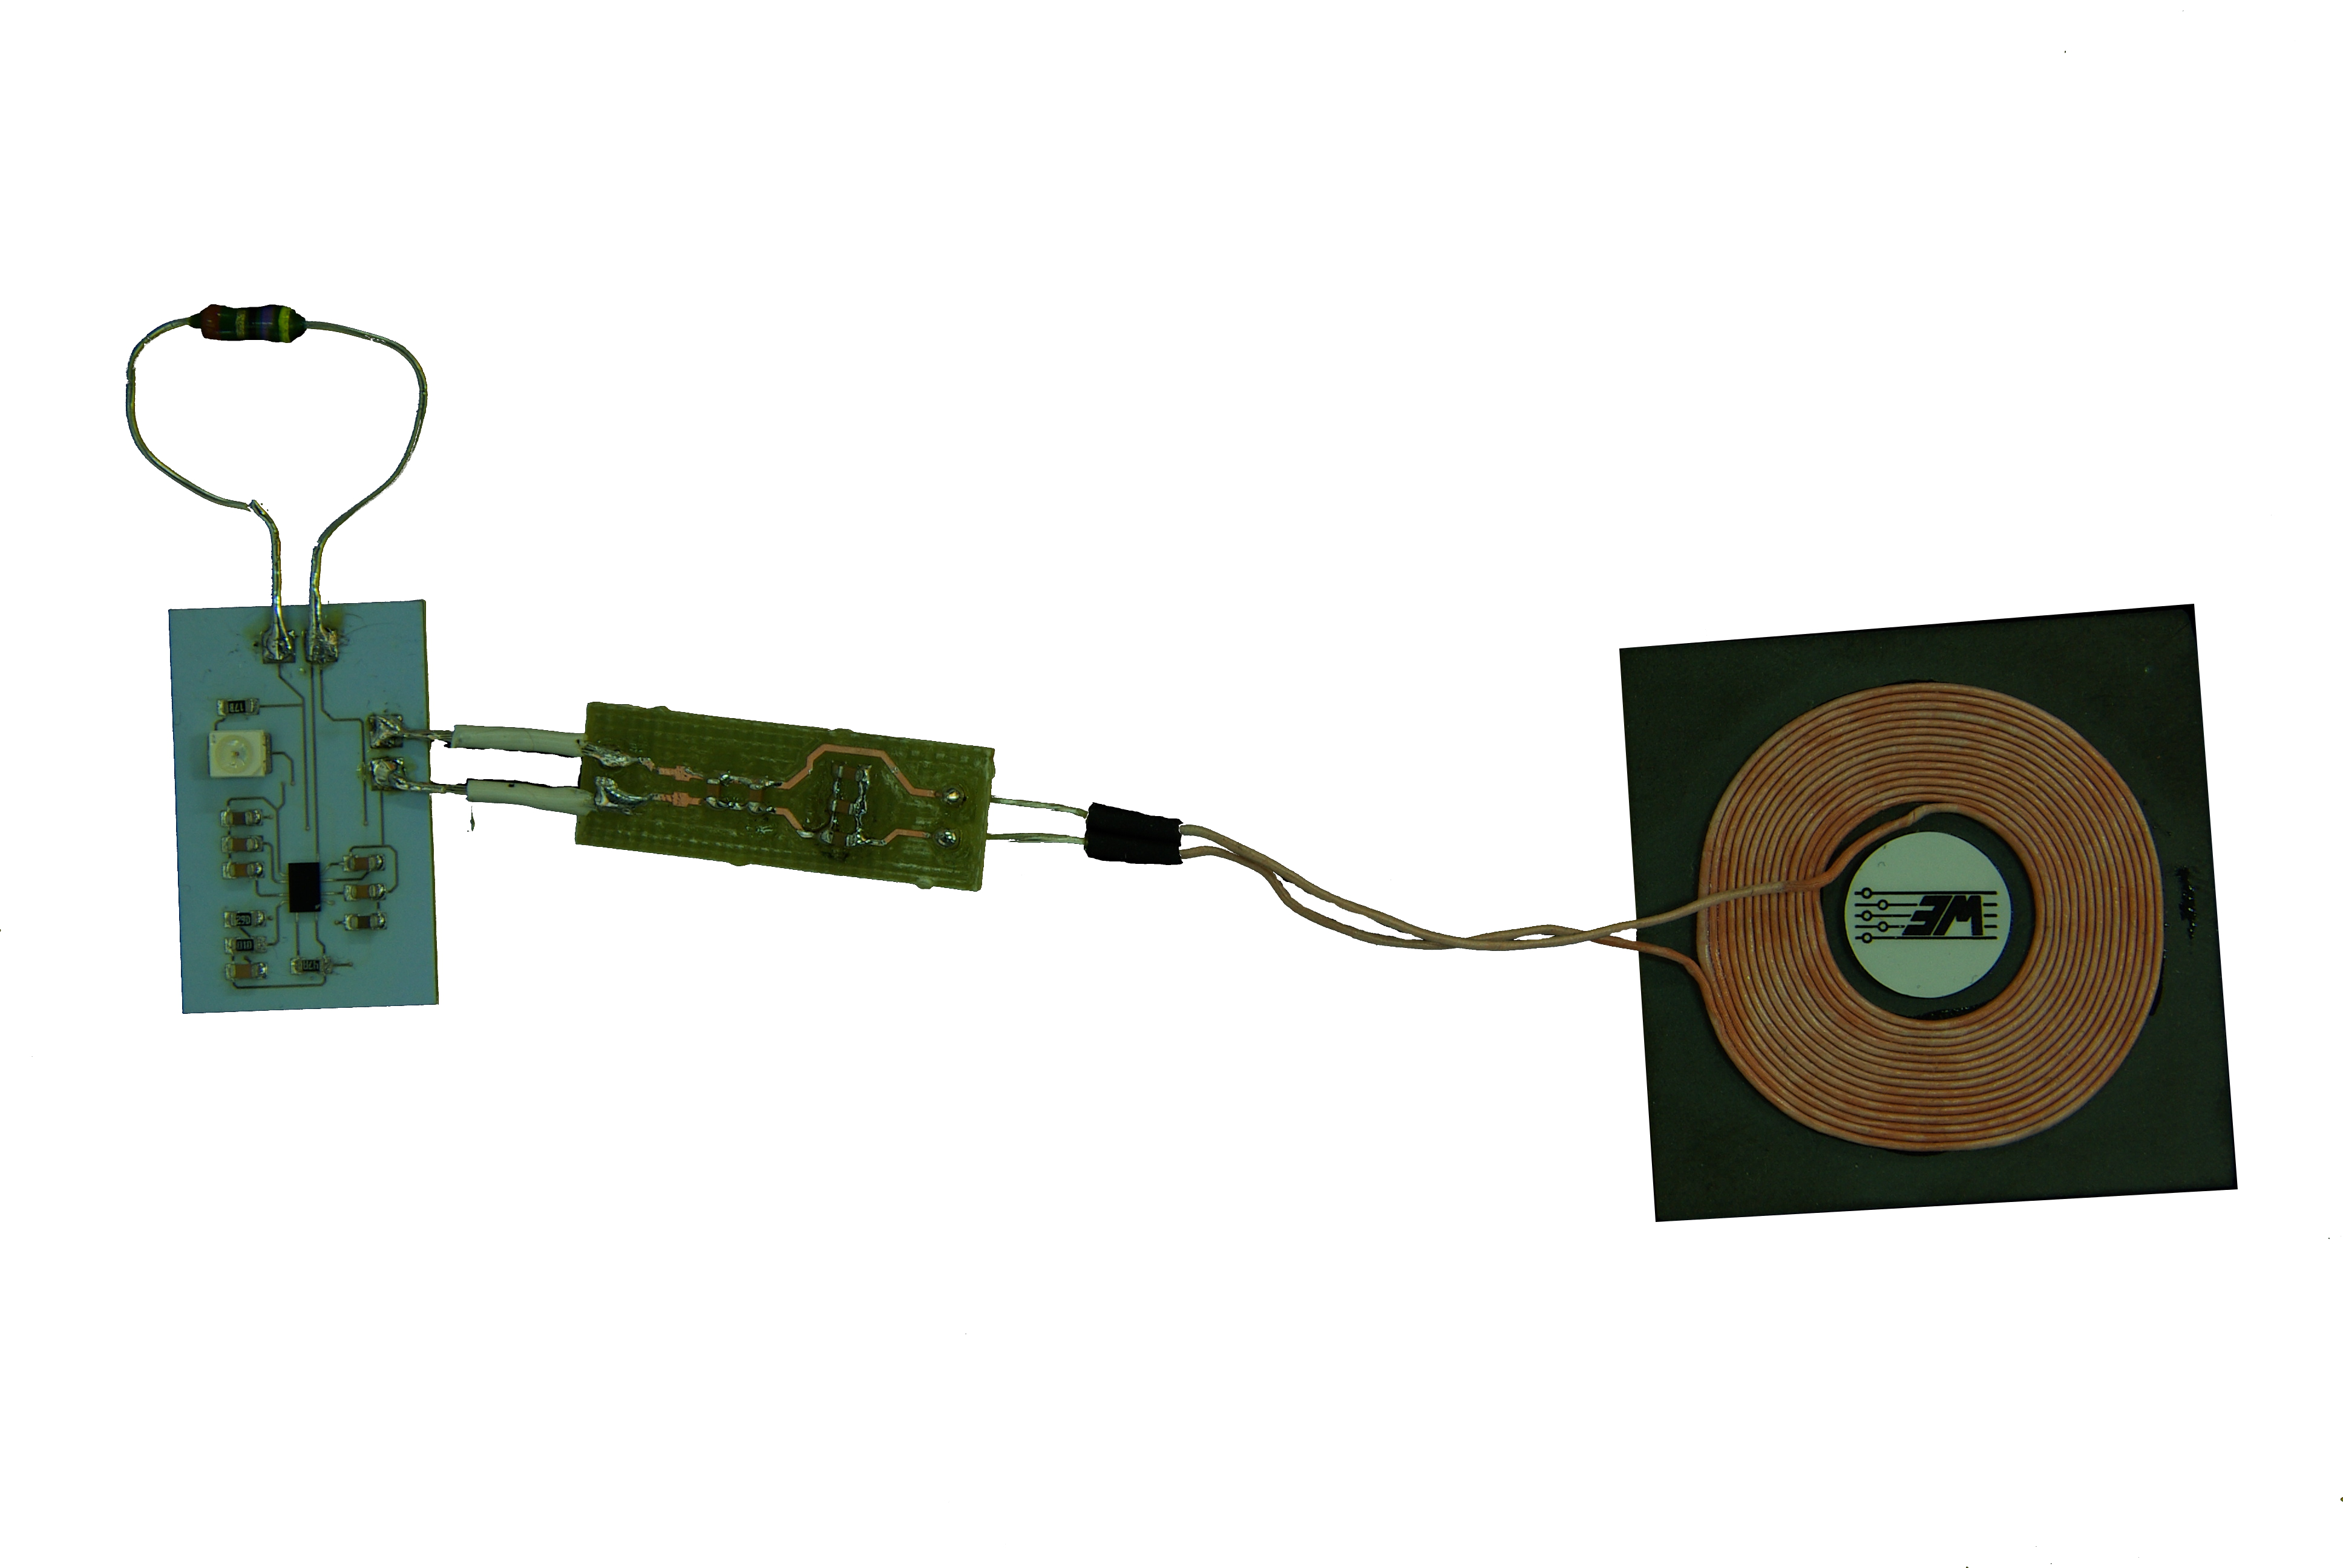
\includegraphics[width=1\textwidth-2\fboxsep-2\fboxrule]{Bilder/self_receiver.JPG}}
Quelle: Stephan Jobstmann
\label{self_rec}
\end{figure}
\section{Energiebereitstellung}
\label{chap:4.2}
Da die Markttauglichkeit bei diesem Projekt eine wesentliche Rolle spielt, wird eine weitverbreitete, einfach zu realisierende und auch günstige Methode gesucht um die Energie für die Elektronik des eingebetteten Moduls bereitzustellen.
\subsection{Superkondensator}
Als Superkondensator werden im Allgemeinen hochkapazitive Energieträger bezeichnet, die Ihre elektrische Ladung anders als Keramik-, Tantal-, Elektrolyt- oder Folienkondensatoren speichern. Sie funktionieren nicht wie diese durch Ladungsseparation mittels Dielektrikum sondern bedienen sich anderer Effekte, wie Energiespeicherung in Helmholtz-Doppelschichten\footnote{Doppelschichtkondensator}, faradayscher Ladungstausch\footnote{Pseudokondensator} oder einer Kombination aus beiden Technologien\footnote{Hybridkondensator}. Aufgrund dieser anderen Bauweisen lassen sich Kapazitäten erreichen, die das von Elektrolytkondensatoren um das 10000-fache überschreiten. Somit ziehen sie bezüglich der Ladungsdichte mit Akkumulatoren gleich. Anders als bei den üblichen Kondensatoren wird durch den technologischen Unterschied der Funktionsprinzipien eine lineare Lade- beziehungsweise Entladekurve erreicht. Weiter In Miniaturbauweise für Platinenmontage sind so ganzzahlige Farad an Ladungskapazität mit dieser Technologie bereits üblich. Für den praktischen Einsatz für die Arbeit fielen diese Energiespeicher aufgrund ihrer schaltungstechnischen Zusatzbeschaltung zur Spannungsstabilisierung und des, im Gegensatz zu den weit verbreiteten Lithium-Ionen Akkus, hohen Kostenfaktors aus. Weiter ist die Selbstentladung zudem höher als bei konventionellen Akkumulatoren. Aus diesen Gründen wurde eine Lösung der Energiezwischenspeicherung, welche auf Superkondensatoren basiert, nicht weiter verfolgt.
\subsection{Lithium-Ionen-Akkumulator}
\label{chap:4.2.2}
 Der Lithium-Ionen-Akku hat sich in den letzten Jahren zur Standardtechnologie für wiederaufladbare Energiespeicher entwickelt. Sie sind in nahezu jedem portablen, elektrisch betriebenen Gerät zu finden. Durch weitere Sicherheitsmaßnahmen, wie den in nahezu allen Li-Ion-Akkus verbauten NTC\footnote{Negative Temperature Coefficient}-Widerstand, der mithilfe externer Sicherheits- und Messbeschaltung Rückschlüsse über die interne Temperaturentwicklung des Energiespeichers schließen lässt. Dies verhindert bei einer Fehlfunktion oder einem Schaden des Akkus einen Brand oder gar eine Explosion des Geräts\footnote{Uelzen: Explodiertes Notebook löst Feuerwehreinsatz aus \citep{tonline}}. \\
Für das Projekt wurde nach einem IC-Baustein gesucht, der selbstständig bei ausreichender Eingangsspannung den Ladungsvorgang bei einem 1-Zellen Li-Ionen Akku vornimmt. Die Wahl eines fertigen ICs bietet einige Vorteile:
\begin{itemize}
\item
Der Aufbau der Schaltung reduziert sich auf ein Minimum an Bauteilen, so werden zum Beispiel Schmitt-Trigger für die Temperaturüberwachung, Spannungsstabilisatoren und Stromquellen bereits in einem Baustein vereint. 
\item
Die Komplexität des Schaltungslayouts wird auf geringen Ausmaßen festgehalten.
\item
Berechnungen zur Auslegung der einzelnen Baugruppen werden obsolet oder auf wenige reduziert. Dabei wird meistens der Anwender durch die im Datenblatt aufgezeigten Anwendungsbeispiele mit Vorlagen zur Berechnung unterstützt.
\item
Die Schaltung ist bereits im Datenblatt festgehalten und muss lediglich bei den Bauteilwerten adaptiert werden.
\end{itemize}
Nach hinreichendem Vergleich fiel die Wahl des zu verwendenden Bausteins auf den BQ24100 von der Firma Texas Instruments\footnote{Battery Management Products - Battery Charger Solutions BQ24100 \citep{TIBQ24100}}. Dieser umfasst eine durch die am Akku anliegende Temperatur gesteuerte Schutzbeschaltung und eine äußerst niedrige Mindestspannung für die Eingangsbeschaltung. Weiter sind diverse Steuereingänge als auch Ausgänge die durch ihre logischen Pegel den aktuellen Status des Ladezyklus wiedergeben im Baustein realisiert. Die Ladelogik erkennt ebenfalls eine Tiefentladung und passt dementsprechend den Ladezyklus an. \\
\\
Berechnungsschritte nach Datenblatt \citep{BQ24100}
\begin{eqnarray}
\Delta I_L &=& I_{Charge} \cdot I_{Charge^{Ripple}}\\
\Delta I_L &=& 1,33 \text{A} \cdot 30 \% = 0,4\text{A}
\end{eqnarray}
\begin{eqnarray}
L_{OUT}&=&\frac{V_{BAT} \cdot \left( V_{INMAX} - V_{BAT} \right)}{V_{INMAX} \cdot f \cdot \Delta I_L}\\
\nonumber\\
L_{OUT}&=&\frac{4,2\text{V}\cdot \left(5\text{V}-4,2\text{V}\right)}{5\text{V} \cdot 1,1 \cdot 10^6 \frac{1}{\text{s}} \cdot 0,4\text{A}}\\
\nonumber\\
L_{OUT}&=&\frac{3,36 \text{V}^2}{2,2 \cdot 10^6  \frac{\text{VA}}{\text{s}}} = 1,527 \mu \frac{\text{Vs}}{\text{A}} = 1,527 \mu \text{H}
\end{eqnarray}
Da das Hybridlabor der Hochschule Landshut während des Aufbaus Induktivitäten mit 6,2$\mu$H im Lager hatte, wurde folgende Rechnung zur Anpassung vorgenommen:
\begin{eqnarray}
\Delta I_L&=&\frac{V_{BAT} \cdot \left( V_{INMAX} - V_{BAT} \right)}{V_{INMAX} \cdot f \cdot L_{OUT}}\\
\nonumber\\
\Delta I_L&=&\frac{4,2\text{V} \cdot \left(5\text{V}-4,2\text{V}\right)}{5\text{V} \cdot 1,1 \cdot 10^6 \frac{1}{\text{s}} \cdot 6,2 \cdot 10^{-6} \frac{\text{Vs}}{\text{A}}} \\
\nonumber\\
\Delta I_L& = & \frac{3,36 \text{V}^2}{34,1 \frac{\text{V}^2\text{s}}{\text{sA}}}=0,0985\text{A} = 98,5\text{mA}\\
\end{eqnarray}
Resultierender Spitzenstrom $I_{IPK}$ an der Induktivität:
\begin{eqnarray}
I_{IPK} &=& I_{OUT}+\frac{\Delta I_L}{2}\\
\nonumber\\
I_{IPK}&=& 1,33\text{A} + \frac{0,0985\text{A}}{2} = 1,379 \text{A}
\end{eqnarray}
Die ideale Ausgangskapazität berechnet sich über eine optimale Resonanzfrequenz von 16kHz. Grundsätzlich bewegt sich die zulässige Frequenz zwischen 8kHz und 32kHz laut Datenblatt \citep{BQ24100}. 
\begin{eqnarray}
f_O&=&\frac{1}{2 \pi \sqrt{L_{OUT} \cdot C_{OUT}}}\\
C_{OUT}&=&\frac{1}{4 \pi^2 \cdot f_O^2 \cdot L_{OUT}}\\
C_{OUT}&=&\frac{1}{4 \pi^2 \cdot \left( 16 \cdot 10^3 \frac{1}{\text{s}} \right)^2 \cdot 6,2 \cdot 10^{-6} \frac{\text{Vs}}{\text{A}}}\\
C_{OUT}&=&1,595 \cdot 10^{-5} \frac{\text{As}}{\text{V}} \Rightarrow 16 \mu \text{F}
\end{eqnarray}
Wieder wurde Aufgrund von Lagerbeständen eine andere Kapazität gewählt: 10$\mu$F 
\begin{eqnarray}
f_O&=&\frac{1}{2 \pi \sqrt{L_{OUT} \cdot C_{OUT}}}\\
f_O&=&\frac{1}{2 \pi \sqrt{6,2 \cdot 10^{-6} \frac{\text{Vs}}{\text{A}} \cdot 10 \cdot 10^{-5} \frac{\text{As}}{\text{V}}}}\\
f_O&=& 20,212\text{kHz}
\end{eqnarray}
Die Resonanzfrequenz der passiven Leistungsbauteile am Schaltungsausgang liegen mit rund 20kHz noch innerhalb des gültigen Bereichs.\\
Der angelegte Speisestrom für den Ladevorgang wird vom IC über einen Shunt-Widerstand $\left( R_{SNS} \right)$ bestimmt. Dieser wird über geforderten Ladestrom $\left( I_{CHARGE} \right)$ und einer Shuntspannung $\left( V_{RSNS} \right)$ dimensioniert. Die Shuntspannung sollte laut Vorgabe zwischen 100mV und 200mV betragen. Für die Berechnung wurde daher ein arithmetisches Mittel von 150mV gewählt.
\begin{eqnarray}
R_{SNS}&=&\frac{V_{RSNS}}{I_{CHARGE}}\\
\nonumber\\
R_{SNS}&=&\frac{150\text{mV}}{1,33\text{A}} = 0,1128 \Omega \Rightarrow 0,1 \Omega \\
\nonumber\\
&&\textrm{resultierende Shuntspannung} \nonumber \\
&&\textrm{bei einem Widerstand von } 0,1 \Omega : \nonumber \\
\nonumber\\
V_{RSNS}&=&R_{SNS} \cdot I_{CHARGE} = 0,1 \Omega \cdot 1,33\text{A} \Rightarrow 133\text{mV}
\end{eqnarray}
Berechnung der Verlustleistung am Shuntwiderstand:
\begin{eqnarray}
P_{RSNS}&=& I_{CHARGE}^2 \cdot R_{SNS}\\
P_{RSNS}&=& \left( 1,33\text{A} \right)^2 \cdot 0,1 \Omega = 176,9\text{mW}
\end{eqnarray}
Die Steuerwiderstände für die Stromgrenzen berechnen sich wie folgt:
\begin{eqnarray}
R_{ISET1}&=&\frac{K_{ISET1} \cdot V_{ISET1}}{R_{SNS} \cdot I_{CHARGE}}\\
 \nonumber \\
R_{ISET1}&=&\frac{1000 \frac{\text{V}}{\text{A}} \cdot 1,0\text{V}}{0,1\Omega \cdot 1,33\text{A}}\\
 \nonumber \\
R_{ISET1}&=&7,5\text{k}\Omega
\end{eqnarray}
\begin{eqnarray}
R_{ISET2}&=&\frac{K_{ISET2} \cdot V_{ISET2}}{R_{SNS} \cdot I_{PRECHARGE}}\\
 \nonumber \\
R_{ISET2}&=&\frac{1000 \frac{\text{V}}{\text{A}} \cdot 0,1\text{V}}{0,1\Omega \cdot 0,133\text{A}}\\
 \nonumber \\
R_{ISET2}&=&7,5\text{k}\Omega
\end{eqnarray}
Das IC verfügt ebenfalls über eine zeitgesteuerte Sicherheitsabschaltung. Dessen Zeitintervall wird über einen externen Kondensator eingestellt.Im Allgemeinen ist von einer sicheren Ladezeit von 5 Stunden auszugehen. 
\begin{eqnarray}
C_{TTC}&=&\frac{t_{CHARGE}}{K_{TTC}}\\
\nonumber\\
C_{TTC}&=&\frac{300 \text{ Minuten} }{2,6 \frac{\text{ Minuten}}{\text{nF}}}\\
\nonumber\\
C_{TTC}&=& 115,4\text{ nF}
\end{eqnarray}
Ähnlich wie im Beispiel des Datenblatts wurde beim Versuchsaufbau der Berechnungsgrundlage ein NTC-Widerstand des Li-Ionen Akkus von 10k$\Omega$  verwendet.\\
\begin{eqnarray}
\text{Mit }&& \nonumber\\
V_{LTF}&=&\frac{V_{O(VTSB)} \cdot \%_{LTF+100}}{100}\\
\nonumber\\
V_{LTF}&=&\frac{3,15\text{V} \cdot 73,5\%}{100} = 2,31525\text{V}\\
\nonumber\\
\text{und } && \nonumber\\
V_{HTF}&=&\frac{V_{O(VTSB)} \cdot \%_{HTF+100}}{100}\\
\nonumber\\
V_{HTF}&=&\frac{3,15\text{V} \cdot 34,4\%}{100} = 1,0836\text{V}
\end{eqnarray}
Lassen sich die begrenzenden Widerstände für die interne Sicherheitsschaltung berechnen. Als Grundlage wurden die Werte für die Widerstände vom Datenblatt übernommen: $RTH_{COLD} = 27,28\text{k}\Omega$ und $RTH_{HOT} = 4,912\text{k}\Omega$.
\begin{eqnarray}
RT2&=&\frac{V_{O(VTSB)} \cdot RTH_{COLD} \cdot RTH_{HOT} \cdot \left( \frac{1}{V_{LTF}}-\frac{1}{V_{HTF}}\right)}{RTH_{HOT} \cdot \left( \frac{V_{O(VTSB)}}{V_{HTF}}-1\right)-RTH_{COLD} \cdot \left( \frac{V_{O(VTSB)}}{V_{LTF}}-1 \right)}\\
\nonumber\\
RT2&=&\frac{3,15\text{V} \cdot 27,28\text{k}\Omega \cdot4,912\text{k}\Omega \cdot \left( \frac{1}{2,31525\text{V}}-\frac{1}{1,0836\text{V}}\right)}{4,912\text{k}\Omega \cdot \left( \frac{3,15\text{V}}{1,0836\text{V}}-1\right)-27,28\text{k}\Omega \cdot \left( \frac{3,15\text{V}}{2,31525\text{V}}-1 \right)}\\
\nonumber\\
RT2&=& 442,235 \text{k} \Omega \Rightarrow 442\text{k} \Omega\\
\nonumber\\
RT1&=&\frac{\frac{V_{O(VTSB)}}{V_{LTF}}-1}{\frac{1}{RT2}+\frac{1}{RTH_{COLD}}}\\
\nonumber\\
RT1&=&\frac{\frac{3,15\text{V}}{2,31525\text{V}}-1}{\frac{1}{442\text{k} \Omega}+\frac{1}{27,28\text{k}\Omega}}\\
\nonumber\\
RT1&=&9,263\text{k}\Omega \Rightarrow 9,31\text{k}\Omega
\end{eqnarray}
\\
\\
Ein passendes Schaltungslayout wurde mithilfe des Datenblatts \citep{BQ24100} und der Software Multisim\footnote{Software für den Schaltungsentwurf: NI Multisim \citep{multisim}} erstellt. Nach der Adaption der Schaltung auf ein passendes Layout wurde über einen Leiterplattenhersteller ein Prototyp auf FR4\footnote{Flame Retarding Number 4; Flammhemmendes Substratmaterial auf Epoxydbasis} bestellt. An der Hochschule Landshut wurde dieser per Hand bestückt und mithilfe der Dampfphasenlötanlage fertig gelötet. Für erste Tests wurde ein handelsüblicher Mobiltelefon-Akku der Firma Huawei verwendet. Dieser war bereits geringfügig vorgeladen und besitzt einen internen NTC-Widerstand von 10k$\Omega$. Somit entsprach diese Testumgebung ziemlich dem realen Einsatzgebiet der Ladeschaltung. Über einen fliegenden Aufbau mithilfe einer Experimentierplatine wurde der Akku an die Schaltung angeschlossen. Diese wurde selbst an eine 5V Konstantspannungsquelle angeschlossen, welche während des Versuchs auch im Spannungspegel verändert wurde. Solange sich die anliegende Gleichspannung innerhalb des im Datenblatt vermerkten Intervalls bewegt, zeigen die Indikationsausgänge des ICs einwandfreien Betrieb auf. Die Funktion des Moduls konnte einwandfrei nachgewiesen werden und war stets reproduzierbar. Auch die kombinierbare Funktion mit dem Modul aus Kapitel \vref{chap:4.1.2} wurde erfolgreich getestet.
\section{Arbeitsschaltung}
\subsection{CC2541}
\label{CC2541}
Um die Sensordaten verarbeiten zu können, wird eine Recheneinheit benötigt. Dabei sollte diese neben der Auswertung und Konvertierung auch eine Möglichkeit bereitstellen, Daten drahtlos zu verschicken. Bei der drahtlosen Datenübertragung war eine weitere Maßgabe, dass diese auf einem lizenzfreien ISM\footnote{Industrial Scientific Medical} seine Nachrichten verschickt. In Europa liegen diese auf den Frequenzen 433MHz, 868MHz und 2,4GHz (es gibt noch weitere ISM-Frequenzbereiche, diese sind allerdings die Gängigsten). Durch eine Vorauswahl von einem Mitarbeiter der Firma SRI\footnote{Sri Radio Systems GmbH \citep{sri}} wurde der Mikrocontroller CC2541\footnote{Personal Area Networks - Bluetooth Low Energy Technology - CC2541 \citep{TICC2541}} für erste Layouttests bestimmt. Mithilfe des Controllerdatenblatts \citep{CC2541} wurde eine grundlegende Schaltung aufgebaut. Diese ist in Teilbereiche zu untergliedern:
\begin{itemize}
\item
Eingangsschutzbeschaltung:  "`resetable Fuse"'\footnote{ein temperaturabhängiger Widerstand, zu deutsch: selbstrückstellende Sicherung}, Verpolschutz
\item
DC/DC-Wandler: TPS62730 plus Peripherie
\item
System on a Chip, kurz SoC\footnote{IC, welches Mikrocontroller und komplexe Peripherie auf einem Siliziumträger vereint}, CC2541 mit integrierter Transmitter-Einheit
\item
Balun\footnote{Balanced to unbalanced} plus Antennenkupplung und diskreter Antenne
\item
Piezosignalgeber: MAS6240\footnote{Low Noise/EMI Piezo Buzzer Driver - Micro Analog Systems \citep{MAS}} 
\end{itemize}
Diese Teilgebiete sollen nun im Folgenden noch einzeln näher erklärt werden.
\subsubsection{Eingangsschutzbeschaltung}
Die Eingangsschutzbeschaltung besteht im Wesentlichen aus zwei Komponenten. Zuerst wäre da die "`resetable Fuse"' welche einen zureichenden Schutz gegenüber Überströme bietet. Diese könnten im ungünstigsten Fall den speisenden Akku irreparabel beschädigen oder diesen zerstören. Die selbstrückstellende Sicherung ist im Grunde ein PTC-Widerstand\footnote{Positive Temperature Coefficient; Wert steigt mit steigender Temperatur}. Allerdings hat dieser eine sprungförmige Kennlinie, d. h. ab einem Schwellenwert wird der Widerstand hochohmig, sodass die gesamte Spannung der Schaltung an der Sicherung abfällt.\\
Der zweite Teil wird zum Schutz der elektronischen Schaltung vor Verpolung benötigt. Die Schutzelektronik besteht aus einem P-Kanal-MOSFET\footnote{Metal Oxid Semiconductor Field Effect Transistor} und einem 10k$\Omega$ Widerstand, der dessen Gate-Eingang vor Leistungsspitzen schützt. Die Funktion ist folgende: Damit der Transistor durchschaltet, muss dessen Source ein positiveres elektrisches Potential haben, als das Gate. Letzteres wird grundsätzlich über den Widerstand auf Massepotential gezogen. Bei richtig gepoltem Anschluss des Akkus leitet die Body-oder Bulk-Diode und das positive Potential der Akkuspannung liegt somit auch an Source an. Der Transistor steuert in Folge dessen auf. Bei Verpolung liegt am Gate grundsätzlich das höhere Potential an und auch die Body-Diode sperrt den Stromfluss. Die Schaltung hinter diesem Schutz bleibt im Fehlerfall unbehelligt. 
\subsubsection{DC/DC Wandler}
Da der CC2541 Baustein unabhängig von der Speisespannung nahezu die gleiche Stromaufnahme hat \citep[vgl. S. 21]{CC2541} wird von der Firma Texas Instruments der Einsatz eines TPS62730 Abwärtswandlers vorgeschlagen. Dieser wandelt eingehende Spannungen von 1,9V bis 3,9V auf eine feste Spannung von 2,10V um.  Durch die geringen Verluste durch den hohen Wirkungsgrad des Spannungswandlers (ca. 86\% am aktuellen Arbeitspunkt) bleibt die anfallende Leistung Eingangs- sowie Ausgangsseitig relativ gleich. Dadurch kann resultierend die Stromaufnahme vor dem TPS62730 reduziert werden. Zur Veranschaulichung folgende Beispielrechnung mit Zahlen aus dem Datenblatt:
\begin{eqnarray}
\text{Active-Mode RX,}&&\nonumber\\
\text{ ohne TPS62730}&&\nonumber\\
&:&17,9\text{mA}\nonumber\\
\text{Active-Mode RX,}&&\nonumber\\
\text{ mit TPS62730}&&\nonumber\\
&:&14,7\text{mA}\nonumber\\
\nonumber\\
P_{Controllereingang}&=&U \cdot I\\
P_{Controllereingang}&=&2,1\text{V} \cdot 17,9 \text{mA}\\
P_{Controllereingang}&=&37,59 \text{mW}\\
\nonumber\\
P_{Wandlereingang}&=& U \cdot I\\
P_{Wandlereingang}&=&3\text{V} \cdot 14,7 \text{mA}\\
P_{Wandlereingang}&=&44,1 \text{mW}\\
\nonumber\\
\eta&=&\frac{37,59\text{mW}}{44,1\text{mW}}\\
\eta&=&0,85
\end{eqnarray}
Wie die Rechnung zeigt, bestätigt sich die Vorüberlegung und der 85\%ige Wirkungsgrad fällt mit einen Mehraufwand an Leistung von 6,51mW kaum ins Gewicht. Gravierender ist dabei die Ersparnis in der Stromstärke um 3,2mA. Diese hat eine rechnerische Verlängerung der Akkulaufzeit um 17,8\% zur Folge.
\subsubsection{System on a Chip}
Der CC2541 SoC vereint einen Mikrocontroller mit 8051-Architektur und eine Radiotransmitter-Einheit, welche eine Funkverbindung auf dem 2,4GHz ISM-Band erzeugt. Er ist die zentrale Verarbeitungseinheit des Systems und beherbergt die Arbitrierung der Messdatenverarbeitung und die Datenübermittlung.  Theoretisch ist es auch möglich mit diesem Chip Bluetooth-Übertragungen aufzubauen. Da aber hierfür Lizenzgebühren anfallen würden, wurden im Projekt erst proprietäre Protokolle zum Erstellen einer Funkverbindung angestrebt. Dies ist allerdings Aufgabe einer anderen Abschlussarbeit. Programmiert wird der SoC über eine TI\footnote{Texas Instruments}-Schnittstelle, welche mit deren CC-Debugger\footnote{Debugger and Programmer for RF-System-on-Chips - CC-Debugger \citep{CCDEBUG}} kompatibel ist. Zur Programmierung sind nähere Informationen in Kapitel \vref{Software} zu finden. Zu der peripheren Beschaltung kann noch auf die zwei Quarze eingegangen werden. Diese geben zum einen den Arbeitstakt im aktiven Modus vor (der 32MHz Quarz), zum anderen gibt es für den Low-Power-Mode\footnote{kurz: LPM} einen 32,768kHz Quarz. Dieser birgt den Vorteil, dass bei niedrigeren Taktfrequenzen deutlich weniger Leistung benötigt wird. Weiter wurden vier Portpins (P0.0 - P0.4) zum etwaigen Erweitern der Funktionalität herausgeführt. 
\subsubsection{Balun}
Der Balun samt Filter wurde von dem Referenzdesign übernommen. So konnte die Berechnung der Bauteilwerte umgangen werden. Die Leitungsdimensionierung wurde mit der Software TXLine\footnote{TX-Line: Transmission Line Calculator AWR Corporation \citep{txline}} vorgenommen. Mit diesem Programm lässt sich ohne größere Kenntnis der Berechnungen die Dimension der Leiterbahnführung bestimmen. Abbildung \vref{TXLine} zeigt als Beispiel die Leiterbahnbreitenberechnung für diese Schaltung.
\begin{figure}
\centering
\caption{Programm TXLine; Berechnung der Leiterbahnbreite}
\fbox{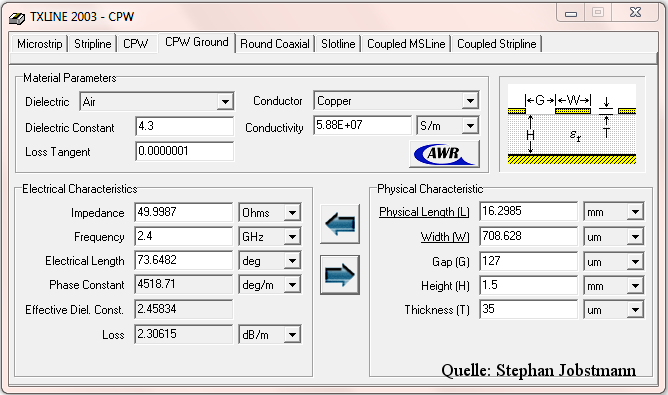
\includegraphics[width=1\textwidth-2\fboxsep-2\fboxrule]{Bilder/TXLine.png}}
Quelle: Stephan Jobstmann
\label{TXLine}
\end{figure}
\subsubsection{Piezosignalgeber}
Als zusätzliches Element soll die Schaltung über einen akustischen Signalgeber Warnhinweise an den Patienten bei akuter Überbelastung ausgeben. Hierfür soll ein Piezobuzzer, wie er beispielsweise in Weckern oder digitalen Armbanduhren verwendet, wird angefügt werden. Der nötigen Spannungshub an dem hochohmigen Eingangswiderstand des Piezokristalls wird über einen Treiberbaustein erzeugt. Der MAS6240 befindet sich seit Längerem im Hybridlabor der Hochschule Landshut im Einsatz. Lediglich die korrekte Ansteuerung über Software fehlte bisher für eine erfolgreiche Inbetriebnahme. Das IC hat eine integrierte dreistufige Ladungspumpe, welche die Eingangsspannung von 3V auf 18$\text{V}_{pp}$ hochzieht. Das Signal wird einfach durch Anlegen der passenden Wechselspannung im für den Menschen hörbaren Bereich erzeugt. Für dieses Projekt wird über eine Zuleitung vom Mikrocontroller eine 4kHz Rechteckspannung angelegt. Diese Frequenz hat weiter den Vorteil, dass sie im psychoakustisch optimalen Bereich der menschlichen Wahrnehmung liegt \citep{Psych}. Hinzukommen noch zwei Steuerleitungen, welche für gewöhnlich ebenfalls vom SoC angesteuert werden sollen, allerdings spielt bei diesem Testaufbau vorerst die Stromaufnahme keine allzu große Rolle. Darum wurden diese Steuereingänge für dauerhaften Betrieb schaltungstechnisch auf High-Pegel gelegt. Weiter enthalten Rechtecksignale Oberschwingungen, die für den Menschen ab einem gewissen Klirrfaktor als unangenehm empfunden werden. Dieser Effekt ist besonders für Warnsignale sehr hilfreich.
\subsubsection{Fazit}
Da sich im Laufe grundlegender Messungen einer anderen Abschlussarbeit herausgestellt hat, dass 2,4GHz äußerst ungünstig als Übertragungsfrequenz für Funkverbindungen in Körpernähe ist, wurde der Aufbau dieses Moduls wieder verworfen und ist somit obsolet. Die Funkverbindung wurde nicht getestet und eine Verbindung mit der Sensorik kam nicht zustande. Lediglich die Ansteuerung und das Layout des Piezotreiberbausteins  wird für zukünftige weiterführende Arbeiten als Grundlage wiederverwendet werden. Ansonsten ist konnten alle erstrebten Funktionen des Moduls (Abbildung \vref{pic.CC2541} erfolgreich im autarken Betrieb validiert werden.
\begin{figure}
\centering
\caption{Modul CC2541; Hergestellt an der Hochschule Landshut}
\fbox{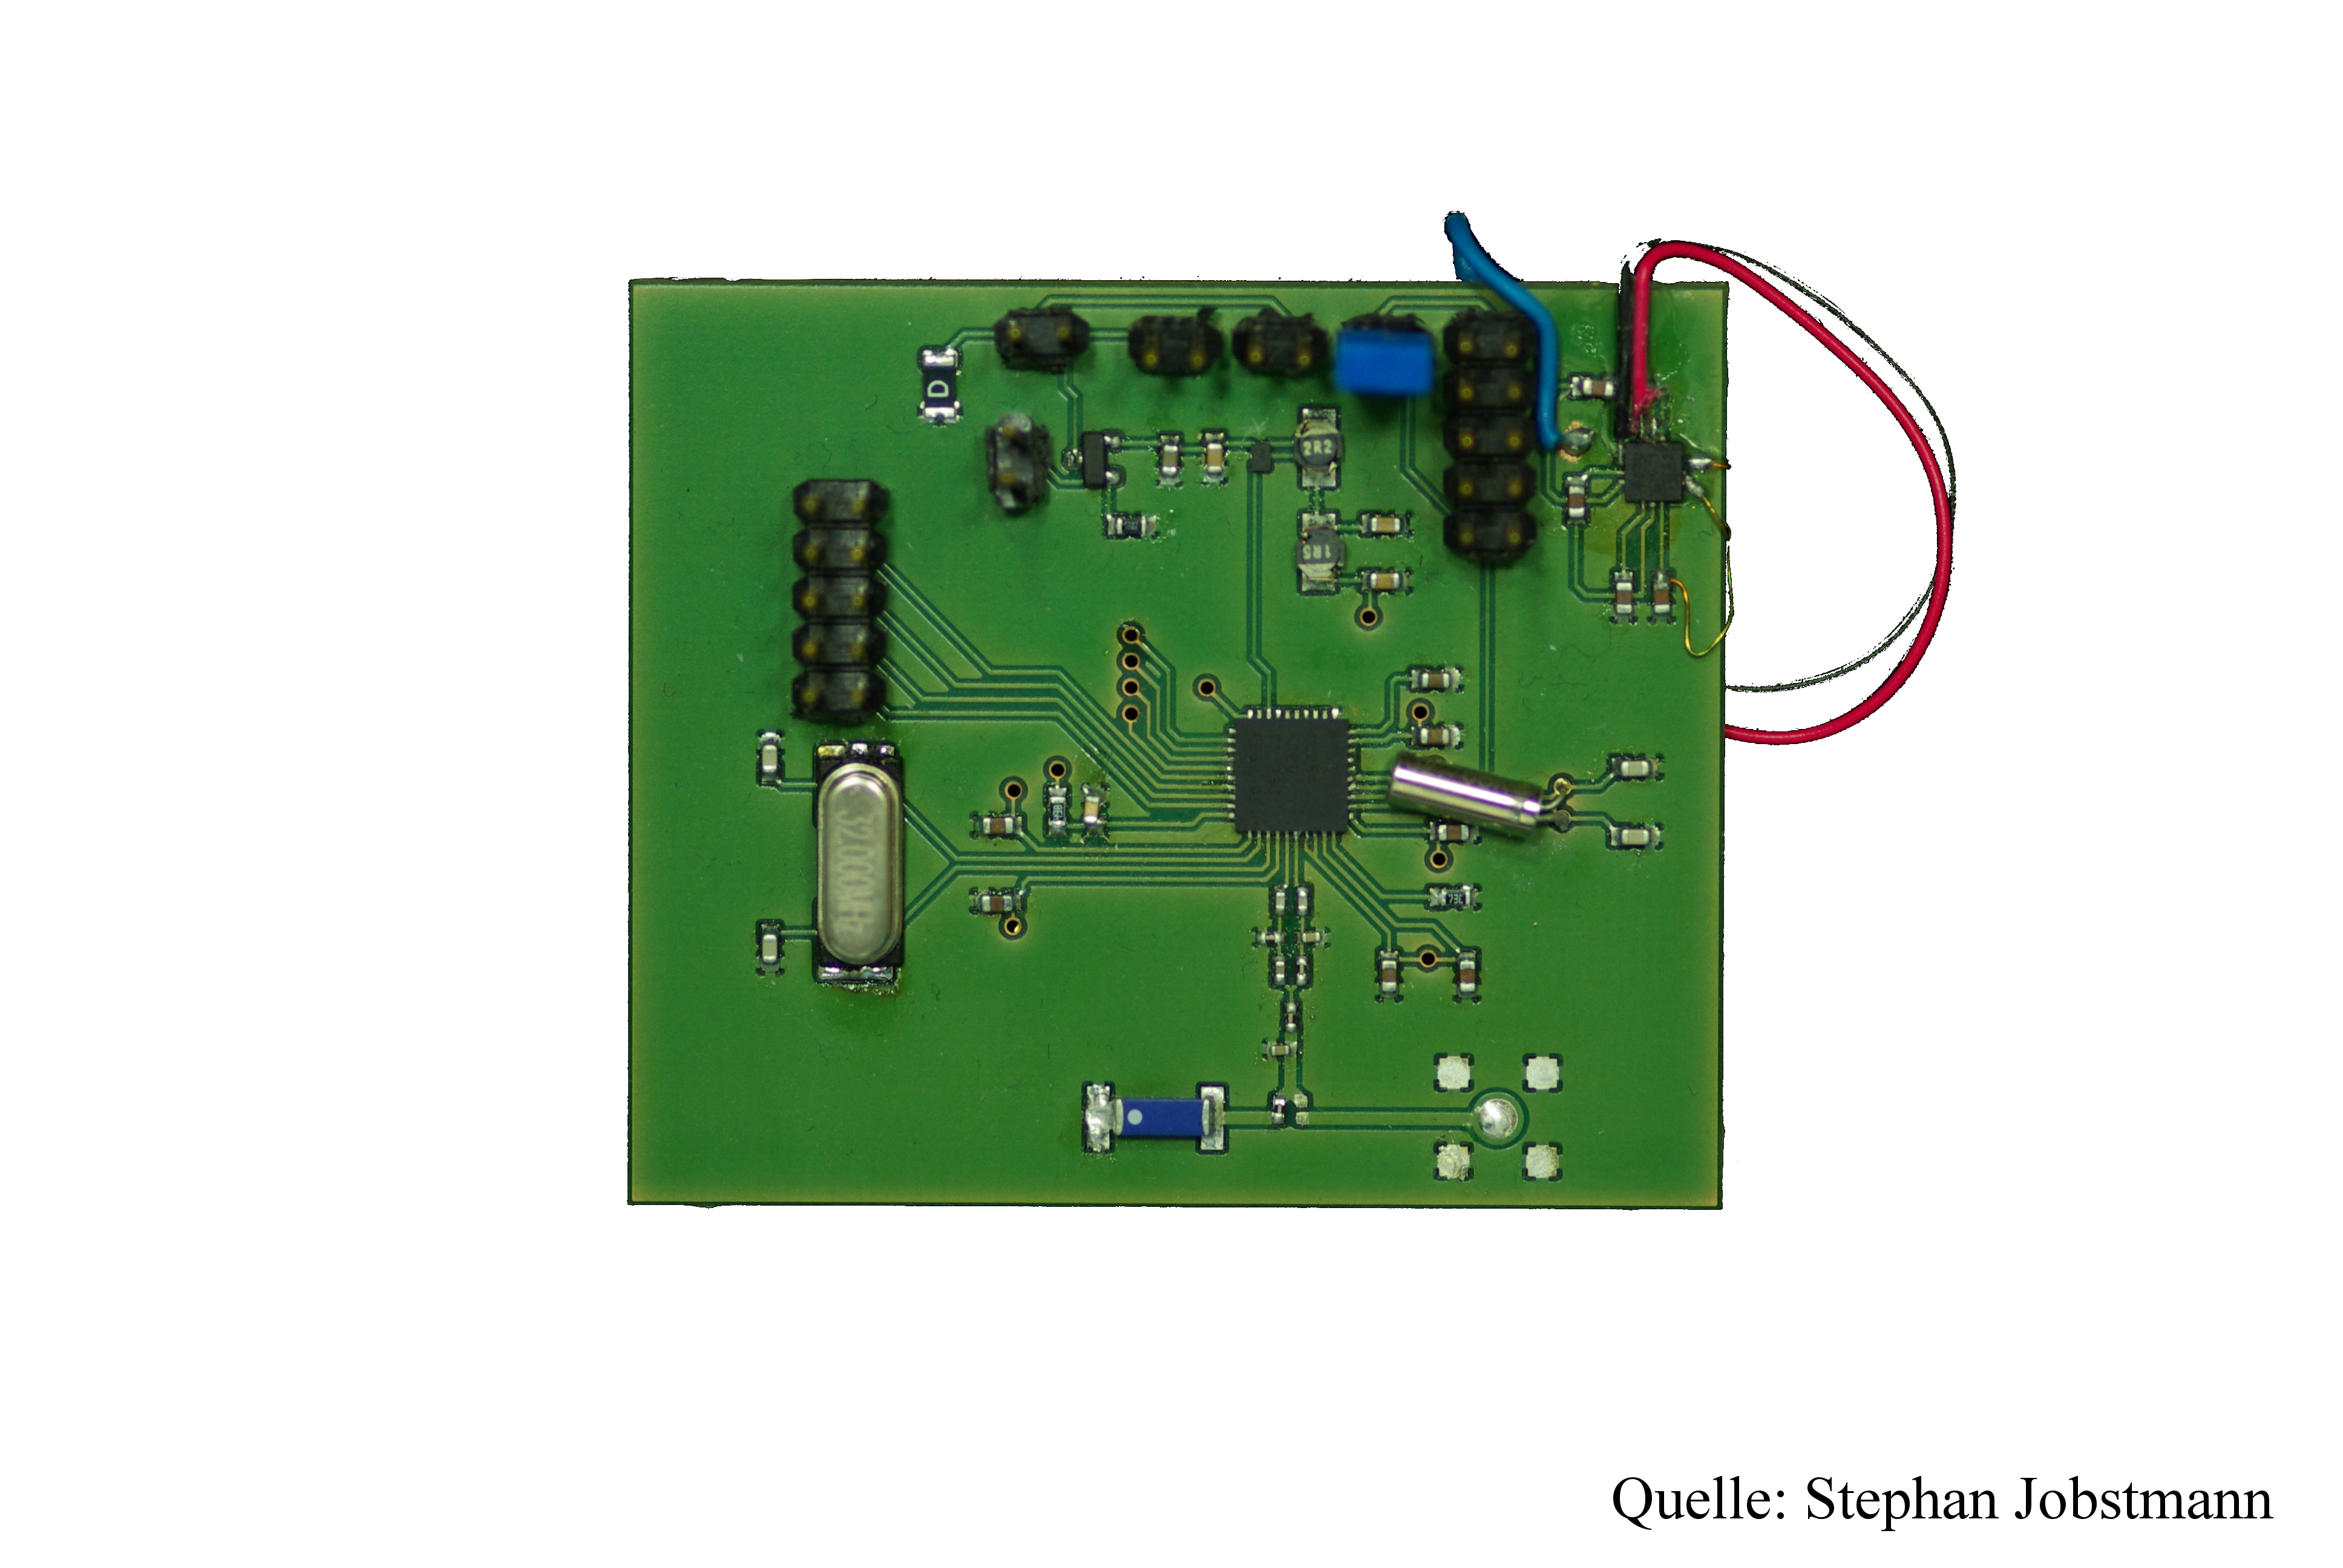
\includegraphics[width=1\textwidth-2\fboxsep-2\fboxrule]{Bilder/CC2541.JPG}}
Quelle: Stephan Jobstmann
\label{pic.CC2541}
\end{figure}
\subsection{CC430F6137}
Genauso wie der CC2541 in Kapitel \vref{CC2541} ist der CC430F6137 ein SoC. Nachdem Ersterer aufgrund seiner schlechten Anpassung der Funkverbindung für den Einsatzzweck für unzureichend eingestuft wurde, sind erste Versuche mit diesem Chip unternommen worden. Dabei wurde vorerst noch keine Modulplatine aufgebaut, sondern eine Entwicklungsplattform von TI verwendet: eine ez430-Chronos Uhr\footnote{EZ430-Chronos Texas Instruments Embedde Processors Wiki \citep{ez430}}. Diese kann je nach Ausführung auf einem ISM-Band eine Funkverbindung mit einer zweiten Uhr oder einer Basisstation aufbauen. Da diese Uhren bereits an der Hochschule Landshut zur Verfügung standen, wurde die Variante mit dem CC430F6137 verwendet.  Dieser ist ähnlich aufgebaut wie der bereits vorgestellte SoC, allerdings wurde hier ein CC1101\footnote{Transceiver Chip von TI \citep{cc1101}} Chip implementiert, welcher auf 868MHz im ISM-Band sendet. Trotz der geringen Abmaße des 64-Pin QFN\footnote{Quadrature Flat No Lead} wurden mit Fädeldraht die Kontakte für die SPI\footnote{serial peripheral interface}-Schnittstelle und für einen Interrupteingang herausgeführt. Dieser wurde mit der im nächsten Unterkapitel (Nummer \vref{Sensorik}) beschriebenen Sensorik verbunden. Schaltungstechnisch ergab sich bei diesem Versuchsaufbau kein allzu großer Mehraufwand. Eine Besonderheit ist die Interruptsteuerung: Anforderung war eine verschleißfreie Möglichkeit den Controller in die Routine für die Datenaufnahme zu überführen. Dabei erwies sich folgender Testaufbau als zielführend:
\begin{itemize}
\item
Für den Taster wurde eine Ersatzschaltung aus einem einfachen Piezobuzzer und einer dazu parallelgeschalteten Zenerdiode (Zenerspannung bei 3,3V) aufgebaut (Siehe Abbildung \vref{pic.breakout}). Der durch einen Druck auf den Piezo erzeugte Spannungshub von mehreren Volt (bis zu 20V) und dessen geringe Ladungsausschüttung genügen zur Signalverarbeitung. Allerdings muss der SoC vor dem großen Spannungspegel wirksam geschützt werden. Darum befindet sich unmittelbar an dem Piezobuzzer gekoppelt eine Diode, welche den anfallenden Pegel auf maximal 3,3V herunterzieht. Da die freigesetzte Ladung des Piezokristalls nicht genügt, um die Diode im Arbeitsbereich zu betreiben, ist beim praktischen Versuchaufbau lediglich Spannungspegel von maximal ca. 2,1V zu erzielen. Dieser reicht aber immer noch aus um eine Flanke bzw. einen Pegel zur Interrupt-Generierung zu erzeugen. 
\begin{figure}
\centering
\caption[Modifizierte ez430-Chronos Uhr]{Modifizierte ez430-Chronos Uhr mit Piezo-Interrupt Taster und Erweiterungsstiftleisten}
\fbox{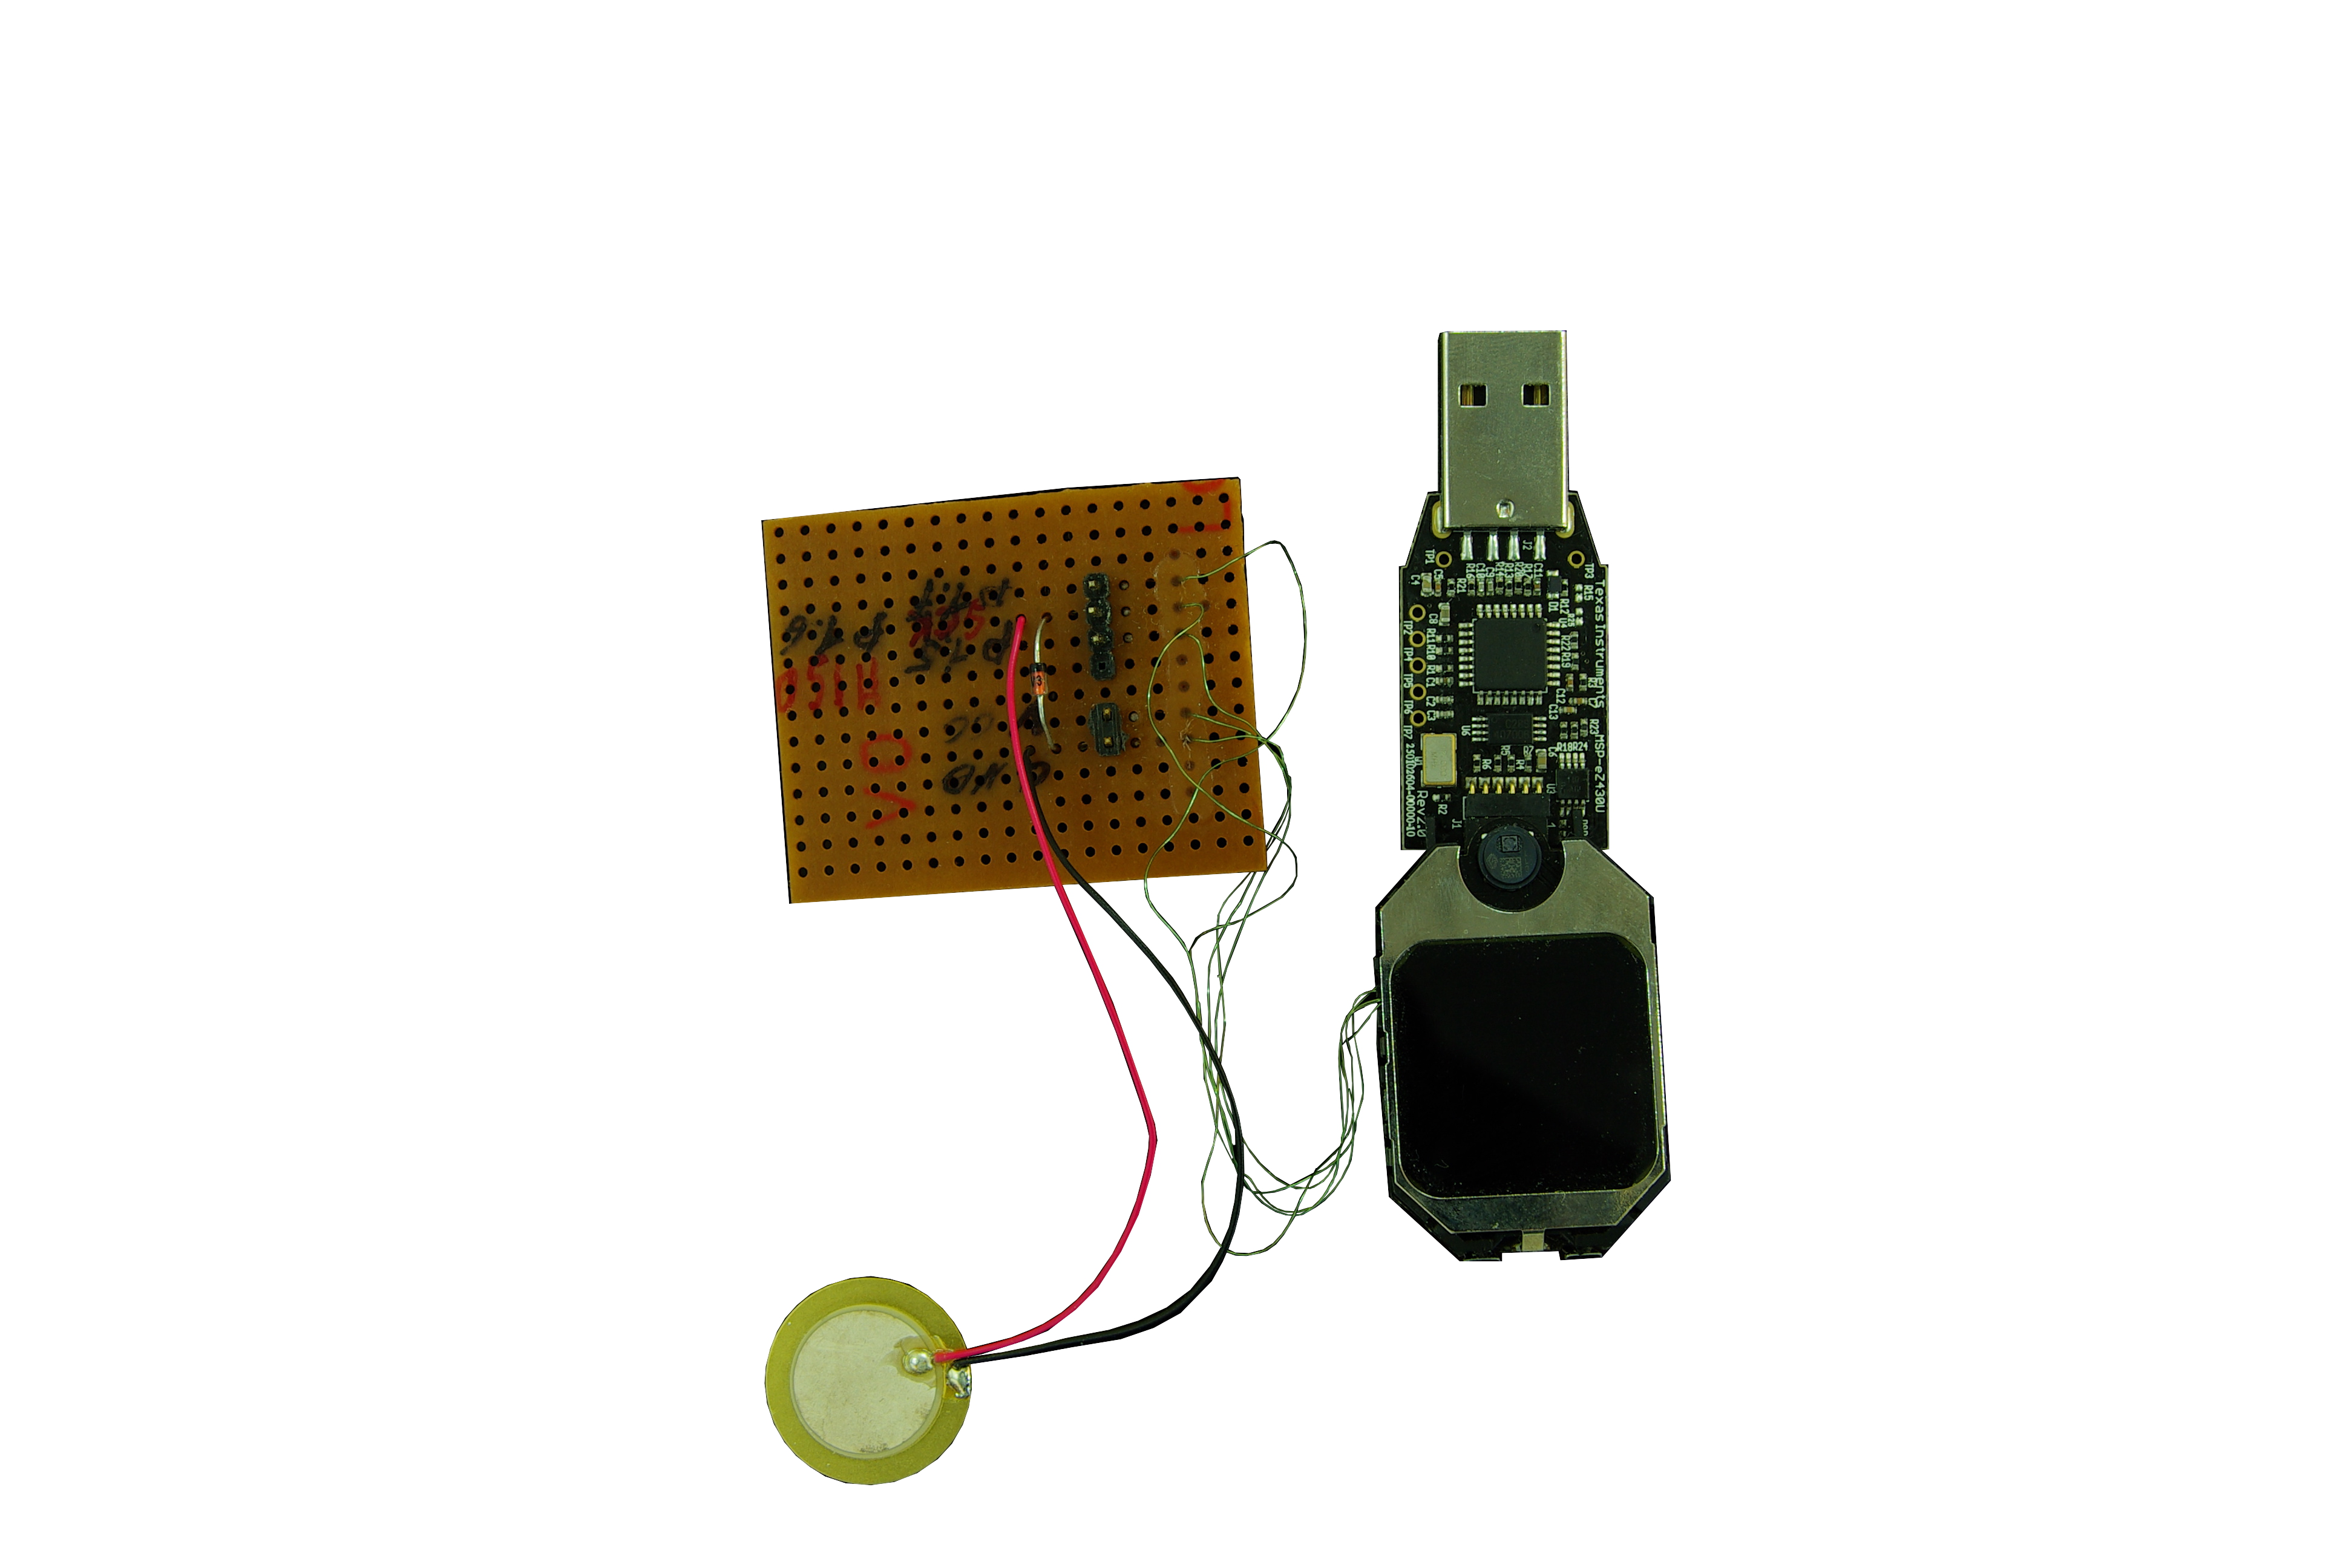
\includegraphics[width=1\textwidth-2\fboxsep-2\fboxrule]{Bilder/breakout.JPG}}
Quelle: Stephan Jobstmann
\label{pic.breakout}
\end{figure}
\end{itemize}
Weiter wurde nach dieser Modifizierung der Entwicklungsplattform auch wieder ein Aufbau in Modulbauweise angestrebt. Dieser hat grundsätzlich die selben Teilbereiche wie der Aufbau des CC2541 in Kapitel \vref{CC2541}. Folgende Unterschiede sind dennoch zu erwähnen:
\begin{itemize}
\item
Neben der üblichen Schnittstelle für den CC-Debugger wurde dieses mal auch eine Flachstecker-Verbindung mit aufgesetzt. Dies ermöglicht eine Programmierung über den Emulationsadapter der ez430-Chronos Entwicklungsplattform.
\item
Es wurden dieses mal gezielt Portpins für die SPI-Verbindung und für den Interrupt-Eingang herausgeführt. Zusätzlich dazu wurde der komplette 8-Bit breite Port 2 auf einer Pfostenleiste zugänglich gemacht.
\item
Es ist kein Low-Power Quarz (32,768kHz) implementiert.
\item
Es wurde auf die Option einer diskret angebrachten Antenne verzichtet. Stattdessen befindet sich zum Testen eine Kupplung für Antennen mit koaxialem Anschluss.
\item
Der Piezosignalgeber wurde für den ersten Prototypen weggelassen. Bei erfolgreichem Aufbau eines Moduls, welches die grundlegenden Funktionen beherrscht wird dieser wieder mit auf die Platine aufgenommen.
\item
der Abwärtswandler wurde aufgrund der mangelnden Empfehlung durch TI nicht integriert. Dieser soll aber beim nächsten Layout ebenfalls als Option bestückbar sein.
\end{itemize}
Die einzelnen Baugruppen sind nach demselben Schema wie dem des Modul des CC2541 aufgebaut. So wurde der Balun und dessen Dimensionierung wieder aus dem Referenz-Design von TI übernommen und die Leiterbahnbreite mit TXLine berechnet. 
Die Verifizierung des Aufbaus (Abbildung \vref{pic.CC430}) konnte aufgrund eines Layoutfehlers am Quarz des CC2541 nicht durchgeführt werden. Es steht ein Redesign für das Schaltungslayout zum Zeitpunkt dieser Arbeit noch aus. 
\begin{figure}
\centering
\caption{Modul CC430F6137; Hergestellt an der Hochschule Landshut}
\fbox{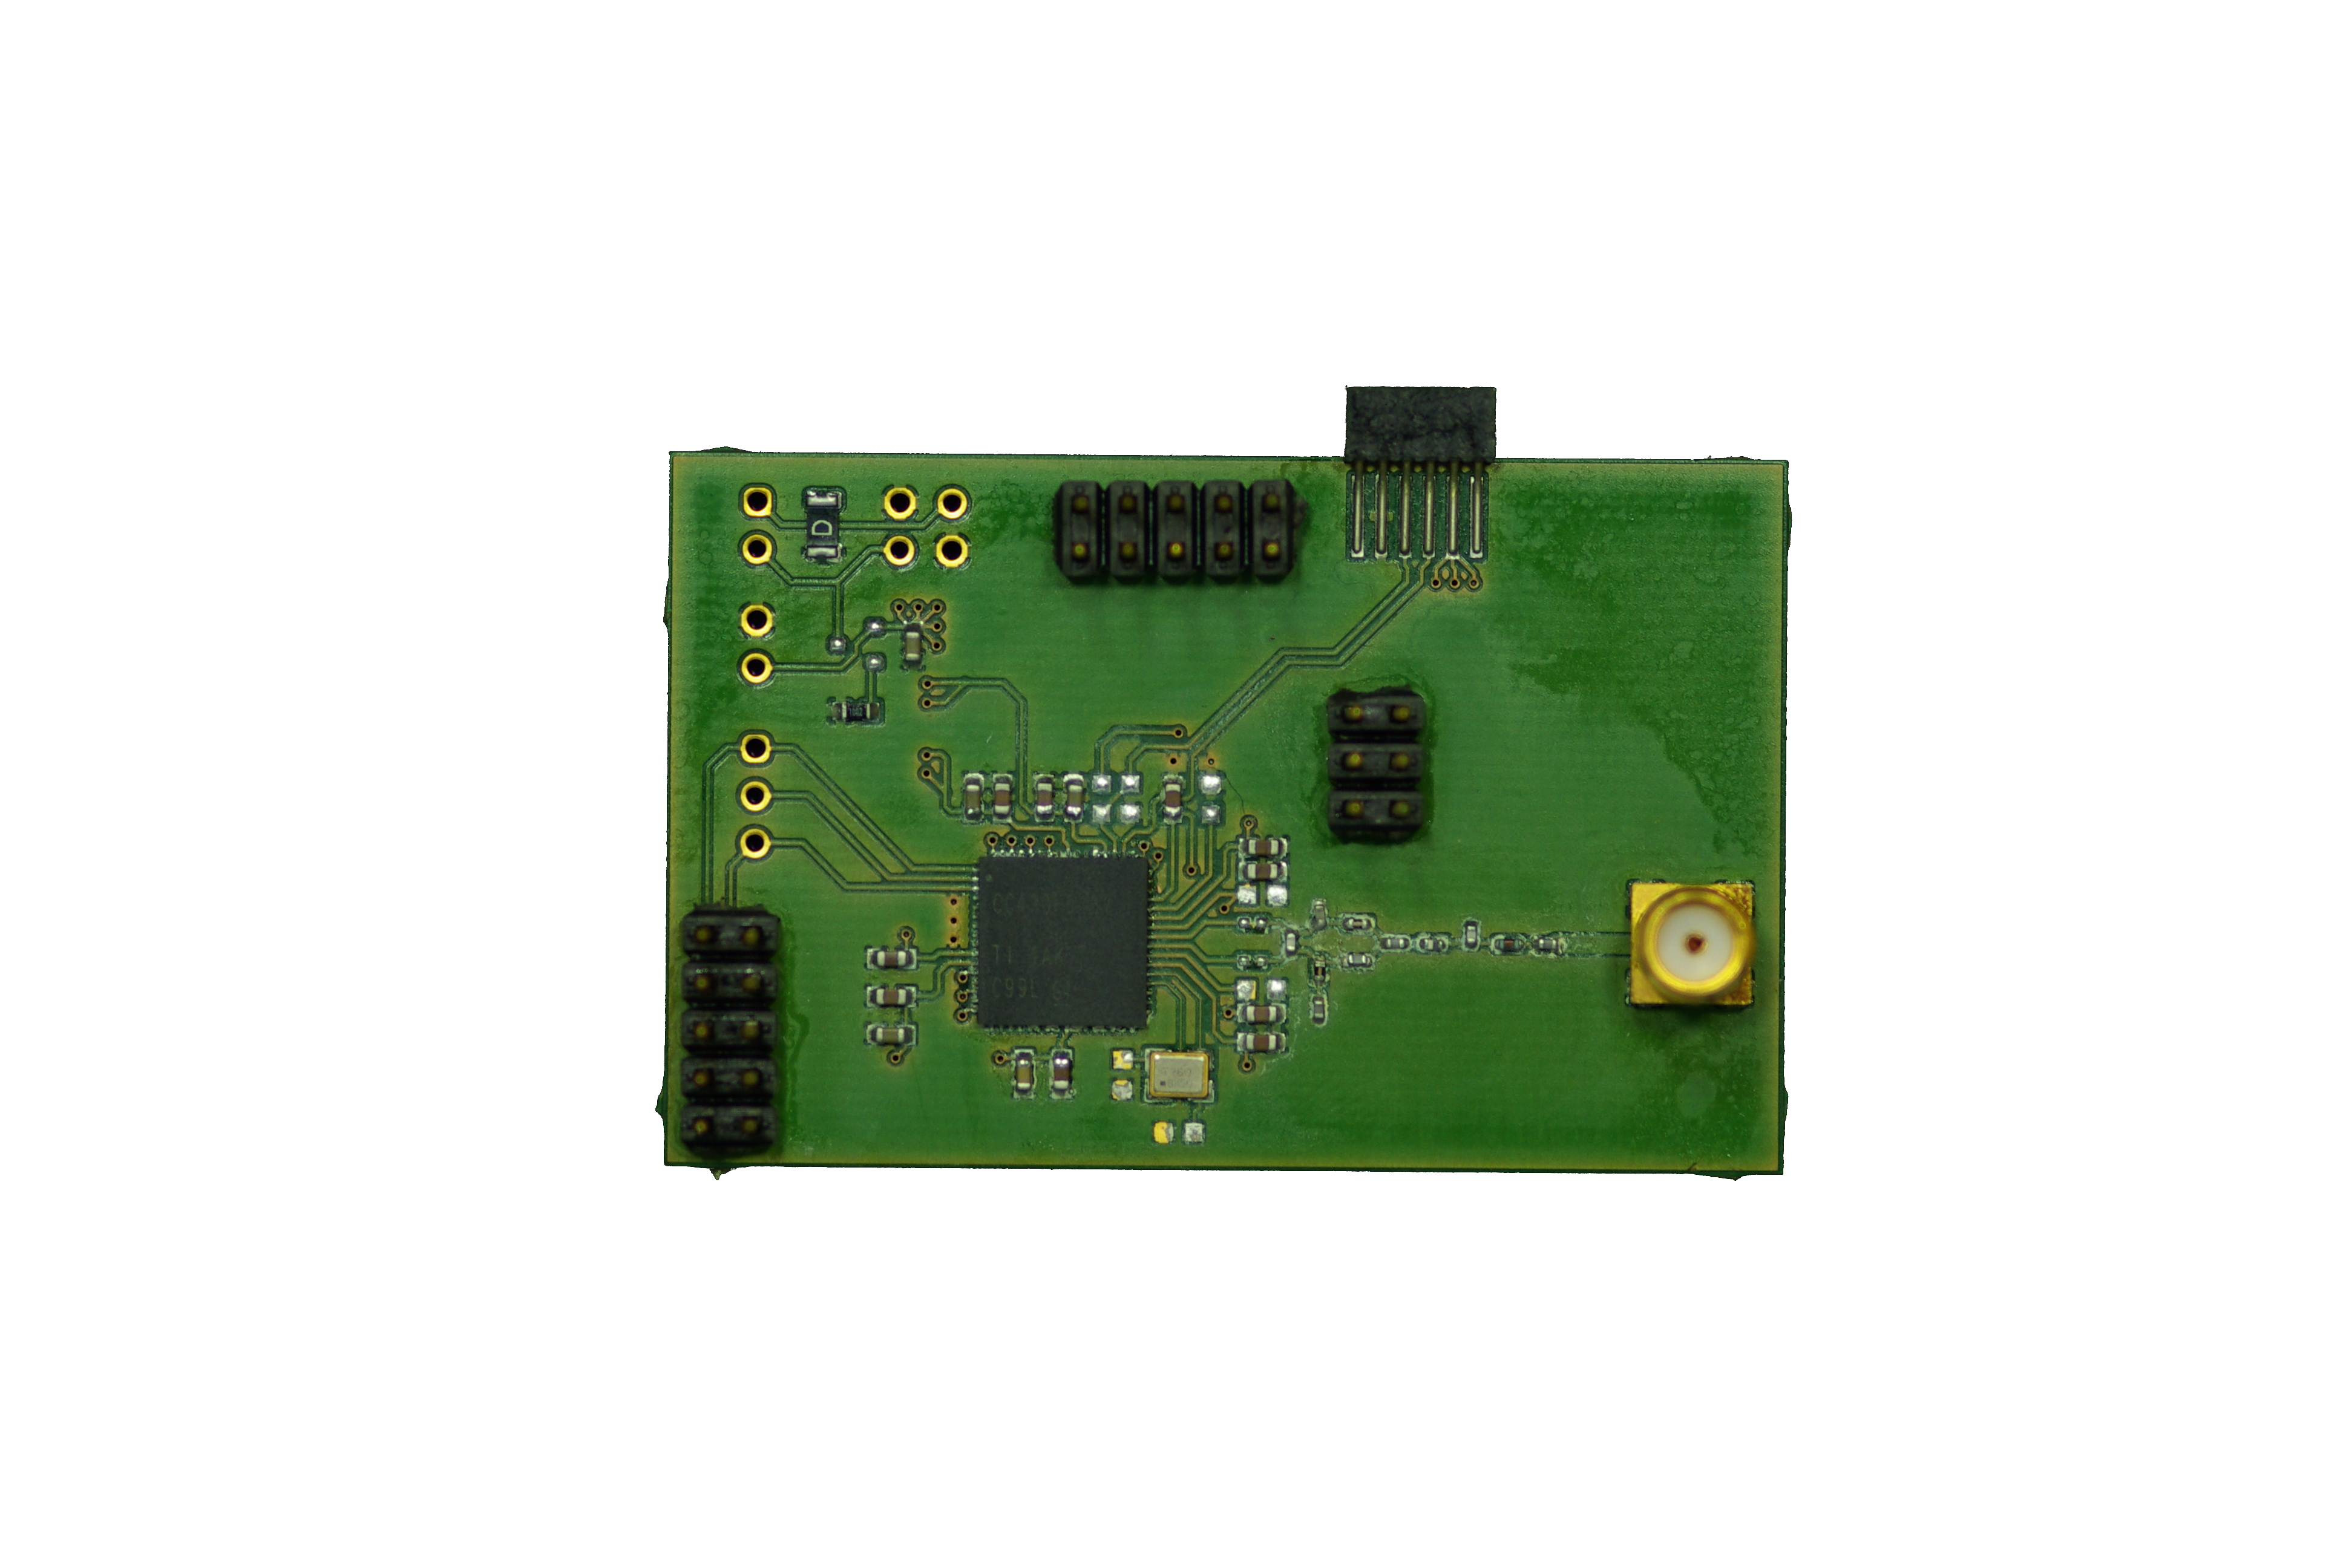
\includegraphics[width=1\textwidth-2\fboxsep-2\fboxrule]{Bilder/CC430.JPG}}
Quelle: Stephan Jobstmann
\label{pic.CC430}
\end{figure}
\subsection{Sensorik}
\label{Sensorik}
Zentrales Element der Schaltung des Fußmoduls des Projekts "`MedLast"' ist der Druckaufnehmer. Erste Versuche die Druckbelastung über die Kapazitätsänderung von Piezoelementen erwiesen sich als äußerst schwierig. Die Problematik bei dieser Messmethode besteht darin, dass sie aufgrund der Flüchtigkeit der geringen Ladung und der Empfindlichkeit gegenüber parasitären Effekten äußerst aufwendig betrieben werden muss, um repräsentative und reproduzierbare Ergebnisse zu erzielen. Als parasitäre Effekte spielen hier unter anderem Luftfeuchte, Beleuchtung und die Umgebungstemperatur eine entscheidende Rolle. Bei ausführlichen Belastungstests im Bereich bis 200N konnten keine zufriedenstellenden Ergebnisse erzielt werden \citep{Jobstmann2012}. Darum wurde die Messmethode auf piezoresistive Dehnungsmessstreifen\footnote{kurz: DMS} geändert. Diese Technologie bietet auch den Vorteil, dass aufgrund der eigenen Verarbeitung im Hybridlabor der Hochschule Landshut das Layout beliebig angepasst werden kann. Da generell davon ausgegangen wurde, dass der Widerstand des DMS sich sowohl vergrößern als auch verkleinern kann, musste das Messverfahren dementsprechend ausgelegt sein. Gemessen wird nicht über eine Kelvin-Messschaltung\footnote{auch bekannt als Vierleitermessung} sondern über eine als Wheatstonesche Brücke bekannte Messschaltung. Dabei wird der betreffende DMS in eine Brückenschaltung, genauer in eine Viertelmessbrücke, eingesetzt. Dies hat zum Vorteil, dass bei richtiger Anpassung der restlichen drei Teilwiderstände der Schaltung, sich an den Messpunkten eine Spannungsdifferenz von $0V$ bei Ruhe einstellt. Aus diesem Grund sollte der zu verwendende A/D\footnote{Analog-Digital}-Wandler die differentielle Spannungsmessung beherrschen oder von vornherein speziell für Messbrückenauswertung ausgelegt sein. Da eine weitere Maßgabe die Auflösung der Wandlung darstellt, wurde explizit nach einem Konverter mit mindestens 12-Bit Auflösung gesucht.\\
All diese Kriterien wurden von dem Baustein ADS1232 von Texas Instruments erfüllt. Dieser verfügt über 24-Bit Auflösung und ist speziell für rein resistive Brückenschaltungen ausgelegt \citep{ADS1232}. Als weiteren Vorteil beinhaltet dieses IC bereits einen internen Temperatursensor der einen der Unterpunkte der Anforderungen an die Arbeit erfüllt.\\
Ein erster Schaltungsentwurf wurde mithilfe des an Hochschule Landshut vorhandenen Leiterplatten-Prototypers\footnote{LPKF C60} auf Platine gebracht, wie auf Abbildung \vref{pic.ad1232}. Dabei wurden alle Konfigurationsmöglichkeiten sowie Ein- und Ausgänge über Jumper und Stiftleisten nach außen geführt:
\begin{figure}
\centering
\caption[AD1232 A/D-Wandler Modul mit Drucksensor]{AD1232 A/D-Wandler Modul mit Drucksensor auf Keramik-Stahl Verbundmaterial}
\fbox{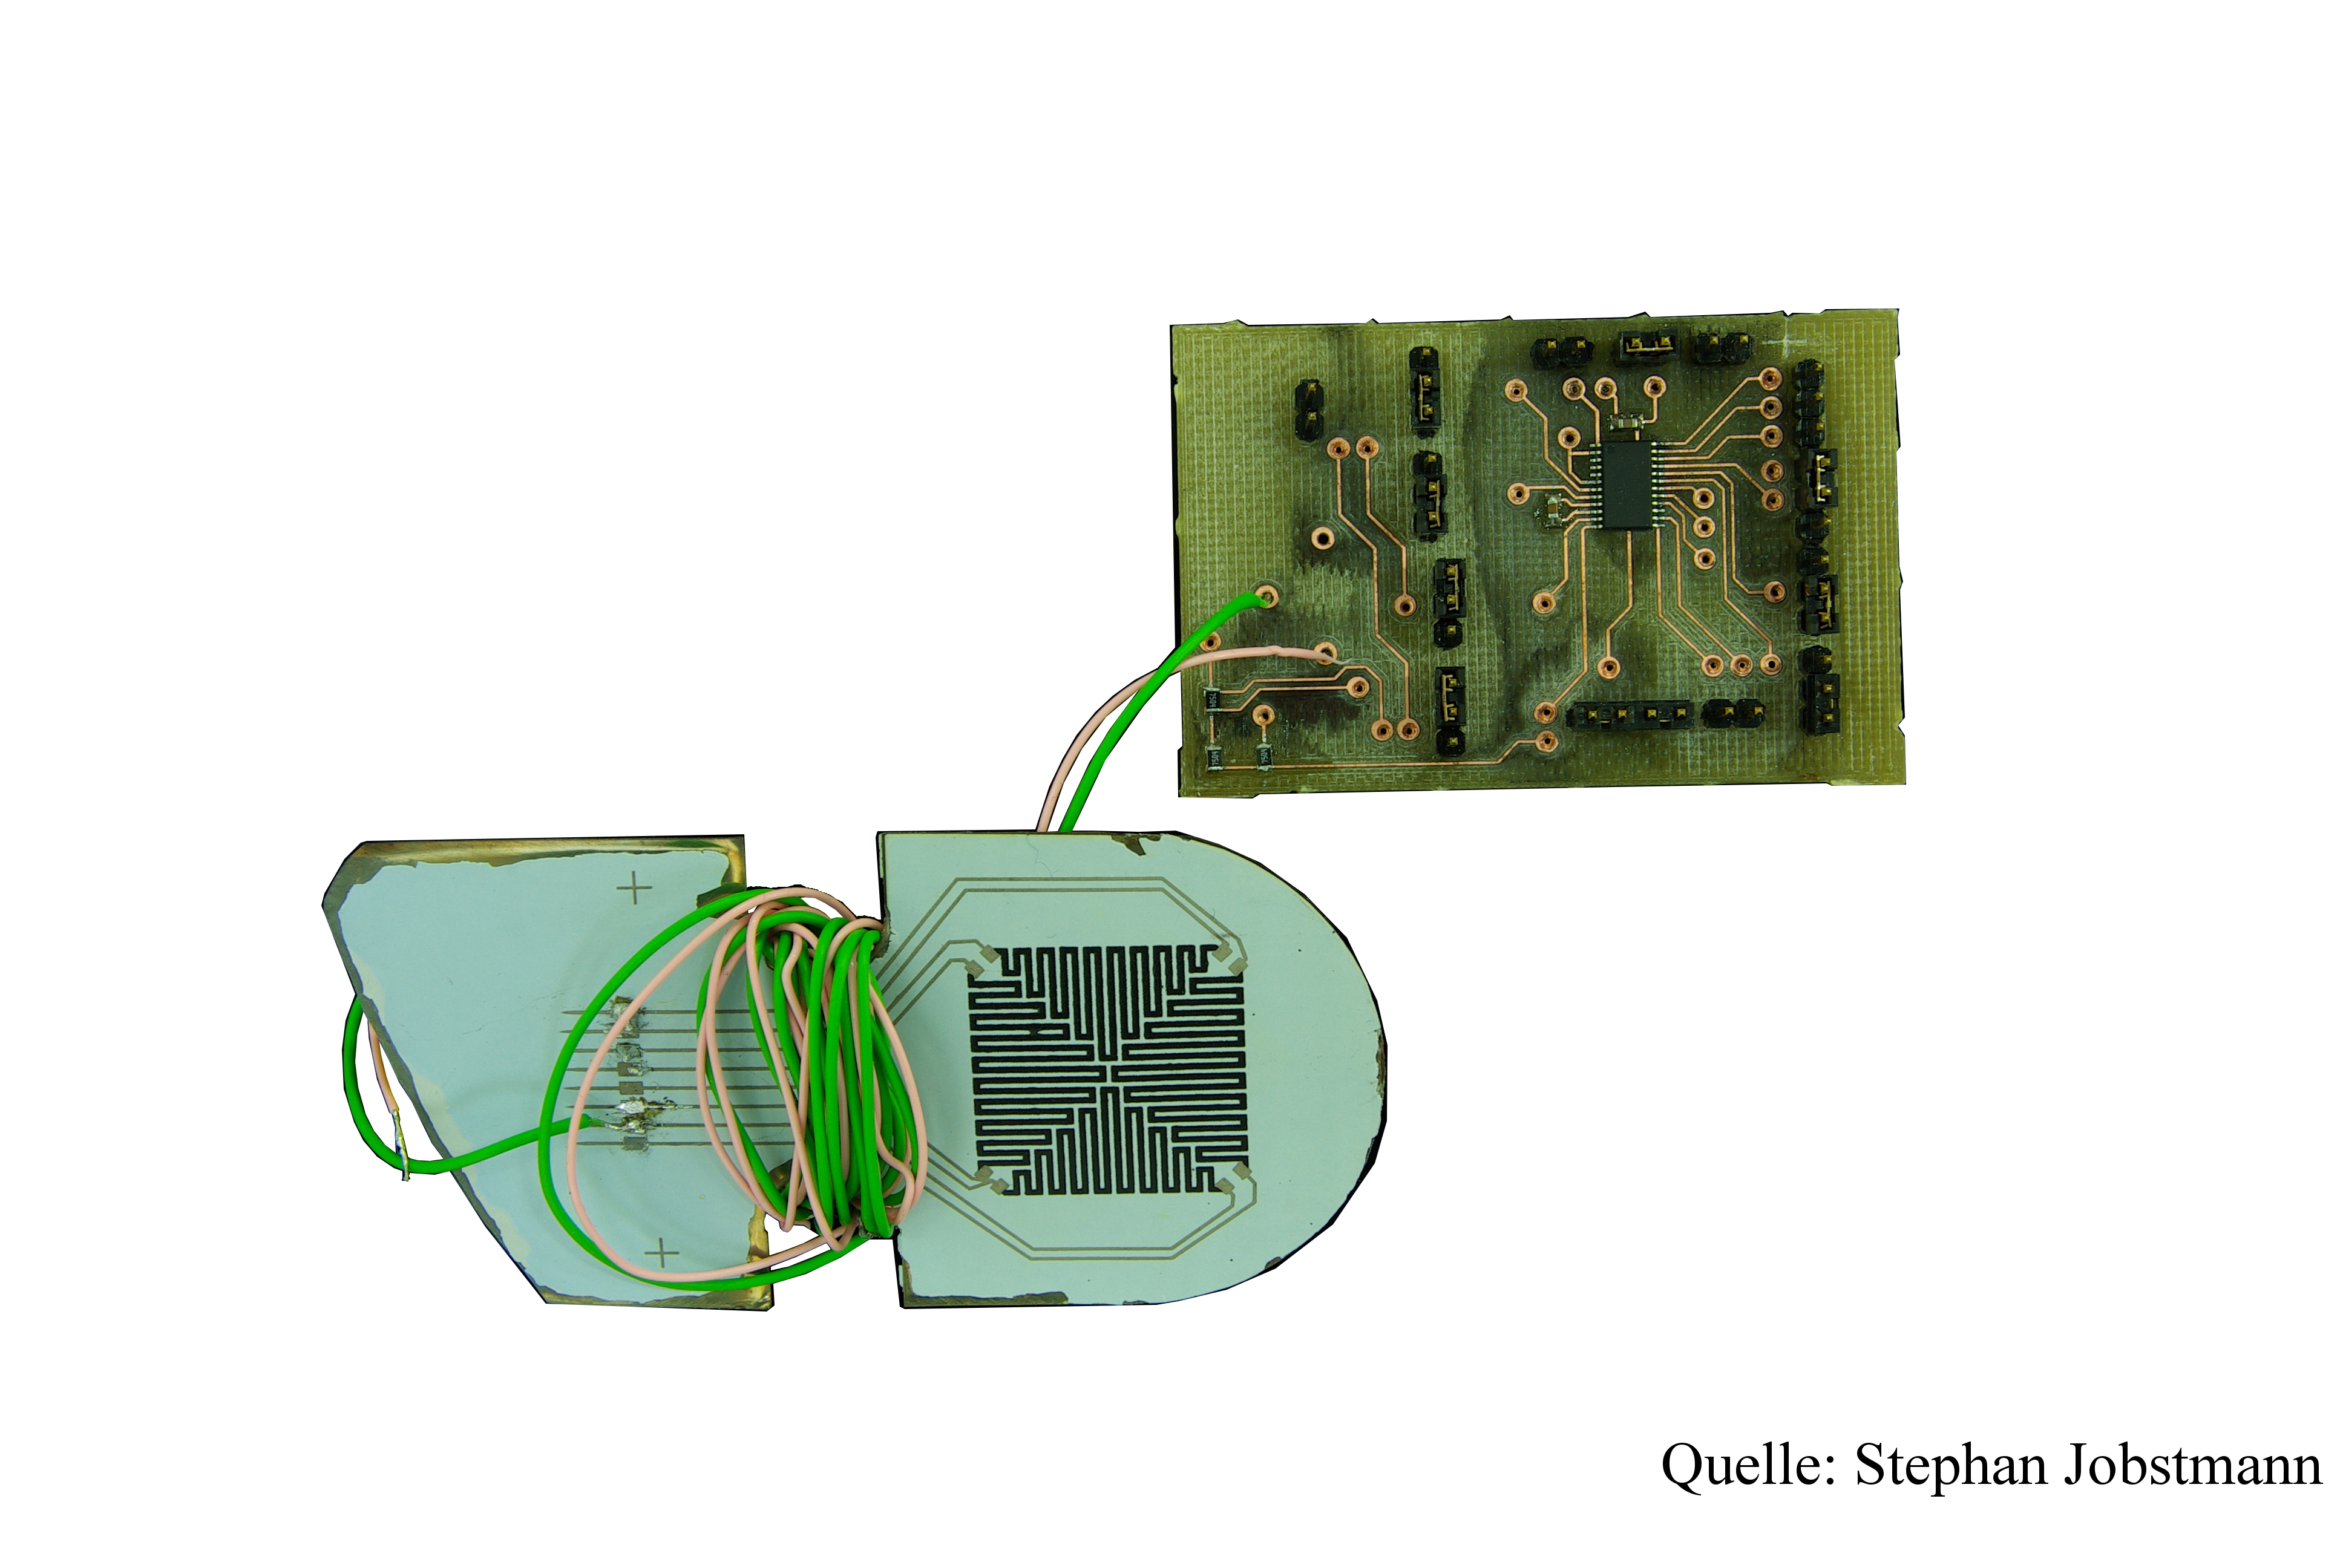
\includegraphics[width=1\textwidth-2\fboxsep-2\fboxrule]{Bilder/ad1232.JPG}}
Quelle: Stephan Jobstmann
\label{pic.ad1232}
\end{figure}
\begin{itemize}
\item
Temperatursensor an/aus
\item
Eingangsbeschaltung: A1/A2
\item
Wandlungsgeschwindigkeit: 10/80 SPS\footnote{samples per second}
\item
Vorverstärkung (Gain 0/1)
\item
Positve sowie Negative Versorgungsspannung
\item
Datenleitungen für SPI
\item
Eingänge für beide analogen Spannungsaufnehmer AIN1/AIN2
\end{itemize}
Da bei der Prototypenschaltung keine allzu gravierenden Spannungs- oder Stromimpulse an der Versorgungsspannung auftreten, können die digitale und die analoge Speisung ebenfalls über einen Jumper zusammengeschlossen werden. Zu Testzwecken wurde eine Viertelbrücke mit einem Potentiometer als variablen Widerstand diskret auf die Platine gebracht. Diese kann über Jumper an den Controller angebunden werden. Für die digitale Anbindung, beispielsweise an einen Mikrocontroller, wird das SPI-Protokoll verwendet. Dabei ist hinzuzufügen, dass lediglich die MISO\footnote{Master Input Slave Output}- und SCK\footnote{Serial Clock}-Leitungen benötigt werden. Zusätzlich verfügt das IC einen PDWN\footnote{Power Down} Eingang, über den der Baustein in einen Ruhemodus versetzt werden kann.\\
Der Testaufbau wurde weiter dahingehend modifiziert, dass es mit einem experimentellen Sensormodul von Frau Engelsberger, basierend auf einem LTCC-Stahl Verbundwerkstoff, optimale Ergebnisse liefert. Dementsprechend wurde die auf dem Modul befindliche Viertelbrücke aufgetrennt und das Potentiometer entfernt. Dieses wurde durch das Sensormodul ersetzt. Weiter wurden die Widerstände der restlichen Brücke an den Sensor angepasst.
\chapter{Software}
\label{Software}
Für diverse Testläufe und die Auswertung der Sensordaten des AD1232-Bausteins sowie der Ansteuerung der erweiterten Peripherie werden verschiedene Programme benötigt. Unter Peripherie ist im Rahmen dieser Arbeit der Piezotreiber und die Interruptsteuerung von externen Signalen zu verstehen. Trotz der verschiedenen Entwicklungsumgebungen haben alle geschriebenen Programme als gemeinsame Sprache \textit{C}. In den folgenden Unterkapiteln werden nur die eigens für diese Arbeit erstellten Routinen und Subroutinen vorgestellt. Falls ein proprietärer Softwarerahmen oder eine Bibliothek vom Hersteller verwendet wurde, ist dies an entsprechender Stelle ausdrücklich erwähnt.
\section{Frequenzgenerierung}
Zur Frequenzgenerierung wurde vorerst als Zielbaustein der CC2541 aufgrund des bestehenden Hardware-Aufbaus (vergleiche Kapitel \vref{CC2541}) in den Vordergrund gerückt. Zum Erstellen wurde die Entwicklungsumgebung IAR Embedded Workbench IDE for 8051\footnote{C/C++ Compiler 8051 - IAR Embedded Workbench for 8051 \citep{iar}} verwendet. Zuerst wurden die grundlegenden Strukturen der Clock-Generierung, der Timer-Funktion und die der Port-Adressierung mithilfe des User's Guide \citep{CC2541_full} ausreichend eruiert. Um den Code auch für Dritte möglichst lesbar zu halten, wurden statt einfachen hexadezimalen Werten zur Registerkonfiguration lesbare Akronyme in einer separaten Header-Datei erstellt. Diese sind ab Seite \pageref{CC2541_porting_defines}zu finden. Der ganze Code wurde wiederum mit Kommentaren versehen um einen schnellen Überblick über dessen Funktion wiederzugeben. Auf Seite \pageref{CC2541_main} ist die Hauptroutine ersichtlich. Von Zeile \texttt{6} bis \texttt{8} wird als Taktquelle für den Prozessor der externe Quarz eingestellt. Die Port-Konfiguration wurde in der Passage von \texttt{10} bis \texttt{13} modifiziert. Dabei wurde die zweite alternative Portbelegung für den Timerausgang vorgenommen. Timer 1 wird in Zeile \texttt{15} mit \texttt{MODULU} zum einfachen Hochzählen bis zu einem festgelegten Wert (Zeile \texttt{22} bis \texttt{24}) konfiguriert. Mit den Passagen \texttt{22}, \texttt{26} bis \texttt{28} wird ein Puls-Breiten-moduliertes\footnote{PWM: Puls Width Modulation} Signal mit 50\% Taktverhältnis erzeugt. 
\newpage
\lstinputlisting[caption={main.c, Umgebung IAR Embedded Workbench for 8051},label=CC2541_main]{main.c}
\newpage
\lstinputlisting[caption={porting\_defines.h, Umgebung IAR Embedded Workbench for 8051},label=CC2541_porting_defines]{porting_defines.h}


\section{Sensorauswertung \& ISR}
Um die Funktion des Sensors festzustellen wurde zunächst eine Plattform gewählt, deren Funktion sich bewährt hat. Somit wurde der AD1232 mit dem 8051 Mikrocontroller Board\footnote{C8051F020 von SiLabs, 8-Bit Mikrocontroller} der Hochschule Landshut in Betrieb genommen. Dies hatte den Vorteil, dass Messwerte über eine bereits im Vorfeld angelegte Code-Bibliothek auf dem LCD\footnote{Liquid Crystal Display} der Zusatzplatine ohne großen Programmieraufwand ausgegeben werden kann. Darum werden im Folgenden auch nur die für den Sensor relevanten Teile erläutert. Auf Seite \pageref{CC430_SPI} werden die Routinen zur Sensordatenverarbeitung der Quelldatei \texttt{SPI.c} dargestellt. Der String am Anfang dient zur etwaigen Ausgabe auf dem LC-Display. Die \lstinline$union$ vereint die einzelnen empfangen 8-Bit Fragmente des ausgelesenen Wertes des 24-Bit A/D-Wandlers zu einem \lstinline$ unsigned long$-Wert (\lstinline{longre}). Über Präprozessor-Anweisungen kann eine Vorselektion der unterschiedlichen Programmabschnitte erzielt werden (\lstinline$MV_OUT, UV_OUT, TEMP, EVAL_BOARD$). So wird ein Großteil des Programmcodes eingespart. Darum kann auch eine Vielzahl an Variationen der Signalaufbereitung in eine Quelldatei untergebracht werden, ohne die maximale Codegröße von 4kByte zu überschreiten. Diese ist von der lizenzfreien Version der Entwicklungsumgebung $\mu$Vision4 von Keil vorgegeben. Im Unterprogramm \lstinline{void wandlascii_signed(unsigned int e)} wird unabhängig von der Vorselektion der empfangene AD-Wert in \texttt{ASCII}-Zeichen umgewandelt. Lediglich die arithmetische Aufbereitung ist unterschiedlich. Ebenfalls ist eine Vorzeichenanalyse allen gemein, diese wird über Bitmanipulation durchgeführt: \lstinline$ken5[x] = (e > 0x7FFF) ? 0x2D : 0x2B;$. Über den Aufruf der Subroutine wird über das Polling-Verfahren der 24-Bit Wert des A/D-Wandlers eingelesen. Dies geschieht über 4 in Reihe folgende Aufrufe einer 8-Bit Empfangsschleife. \\
In der Headerdatei \texttt{dependencies.h} auf Seite \pageref{CC430_dependencies} werden die Anweisungen für den Präprozessor definiert. Dazu kommen noch Kalibrationswerte für den internen Temperatursensor des AD1232, welche durch empirische Analyse festgelegt wurden.
Nach erfolgreicher Inbetriebnahme des A/D-Wandlers mit dem Hochschul-Board, wurde eine Adaption auf die ez-Chronos Uhr vollzogen. Dafür wurde ein Programmbeispiel\footnote{CC430F613x Demo - USCI\_A0, SPI 3-Wire Master Increment Data \citep{cc430f6137}} von Texas Instruments als Grundlage verwendet und dementsprechend angepasst. Um eine eventuelle weitere Portierung zu vereinfachen, beginnt die Quelldatei auf Seite \pageref{CC430_ADS1232} mit \lstinline$#define$-Anweisungen die ein schnelles Angleichen ermöglichen. Nach dem Abschalten des Watchdog-Timers in der \lstinline$void main(void)$-Routine werden die Ports gesetzt und der SPI-Port konfiguriert. Eine Besonderheit des Controllers fällt dabei auf: es ist beim Betrieb der SPI-Schnittstelle nicht nötig, alle drei Standardleitungen (MOSI, MISO, SCK) zu setzen. So kann bei PIN/PORT-Mangel auch beispielsweise ein MOSI-PIN als GPIO\footnote{General Purpose Input Output} verwendet werden, wenn über SPI ausschließlich Daten eingelesen werden. Weiter wird ein Interrupt-Eingang für den Piezo-Taster und der zugehörige Vector eingeschalten. 
In der \lstinline$__interrupt void PORT1_ISR(void)$ (Zeile \texttt{109}) wird mit ankommenden Interrupt zuerst geprüft, ob am A/D-Wandler gültige Daten anliegen. Danach werden wie im vorhergehenden Programm für den 8051 Controller die 4 8-Bit Werte des 24-Bit ADC-Werts eingelesen.
\newpage
\lstinputlisting[caption={SPI.c, Umgebung $\mu$Vision4 Keil},label=CC430_SPI]{SPI.c}
\newpage
\lstinputlisting[caption={dependencies.h, Umgebung $\mu$Vision4 Keil},label=CC430_dependencies]{dependencies.h}
\newpage
\lstinputlisting[caption={ADS1232.c, Umgebung Code Composer Studio v4},label=CC430_ADS1232]{ADS1232.c}
\bibliography{literatur}
\bibliographystyle{alpha}
\end{document}
















